\documentclass[a4paper,11pt,oneside,openany]{jsbook}
\bibliographystyle{junsrt}

%%%%%%%%%%%%%%%%%%%利用パッケージ一覧%%%%%%%%%%%%%%%%%%%
\usepackage[T1]{fontenc}       %Latin Modern
\usepackage{lmodern}           %Latin Modern
\usepackage{amsmath,amssymb}  % 数式用
\usepackage{bm}               % 太文字ベクトル用
\usepackage[dvipdfmx, nosetpagesize]{graphicx} %画像用
\usepackage{subcaption}
\usepackage{amssymb} %チェックマーク用
\usepackage{verbatim}
\usepackage{wrapfig}
\usepackage{ascmac}
\usepackage{makeidx}
\usepackage{fancyhdr}
\usepackage{layout}
\usepackage{caption}  %`キャプションのスタイル用
\usepackage{booktabs} %for table
\usepackage{float}
\usepackage{multienum} %2段組
\usepackage{url}
\usepackage{multirow}
\usepackage{comment}
%%%%%%%%%%%%%%%%%%%ドキュメントスタイル%%%%%%%%%%%%%%%%%%%%
\setcounter{tocdepth}{2} %サブセクションまで目次に表示する
\makeindex
%
\setlength{\textwidth}{\fullwidth}
\setlength{\textheight}{41\baselineskip}
\addtolength{\textheight}{\topskip}
\setlength{\voffset}{-0.55in}

%%%% ヘッダー・フッターの設定 %%%%
\pagestyle{fancy}
\lhead{\rightmark}
\rfoot{\thepage}
\cfoot{}
\renewcommand{\chaptermark}[1]{\markboth{第\ \normalfont\thechapter\ 章~#1}{}}
\renewcommand{\sectionmark}[1]{\markright{\thesection #1}{}}
%\renewcommand{\footrulewidth}{0.4pt}


%%%%%%%%%%%%%%%%%%ドキュメント開始%%%%%%%%%%%%%%%%%%%%%
\begin{document}
\frontmatter

%目次のカウント開始
\tableofcontents
\thispagestyle{fancy}
%
%本文開始
\mainmatter

%%%%%%%%%%%%%%%%%%%%%%本文%%%%%%%%%%%%%%%%%%%%%%%%%
% 1.序論
\chapter{序論}
\thispagestyle{fancy} %ヘッダー・フッターの設定

% 「。」を「.」にしたり、「、」を「,」にしたりするのは後で置換で一括でやります。

ここでは、医療画像レジストレーションの概要及びその問題点を述べ、研究目的について述べる。

\section{医療画像レジストレーション}
    現在の医療において,医用画像処理技術は検査から手術まであらゆる場面で利用されている.
医療画像レジストレーション(Medical Image Registration)は数ある医用画像処理技術のうちの一つであり,画像融合,画像マッチングとも呼ばれる.
この画像レジストレーションは,2つ以上の画像を内容が一致するように一つの座標系に変換する操作のことであり,特に医用画像においては,複数の画像を解剖学的構造が一致するように変換する操作のことを指す.
この技術は,画像ガイド下手術,臓器の変形追跡,線量蓄積,腫瘍成長モニタリングなどの,多くの臨床タスクに必要不可欠である.

\subsection{活用事例}
    例えば、前立腺におけるMRI-TRUS融合画像ガイド下生検\cite{marks2013mri}の場合、解像度に優れたMR画像と、リアルタイム性に優れたUS画像が同時に用いられる。
    事前にMRIを用いて腫瘍の位置をマーキングした後に、USを用いたリアルタイムな撮像の映像と重ね合わせることにより、USの解像度の低さを補完し、腫瘍の箇所を判別するために医療画像レジストレーションが用いられる。
    この画像ガイド下生検では、生検の精度が優位に向上することが知られており\cite{shoji2015manually}、本技術が治療精度向上に貢献可能であることは明らかである。
    \begin{figure}[ht]
      \centering
      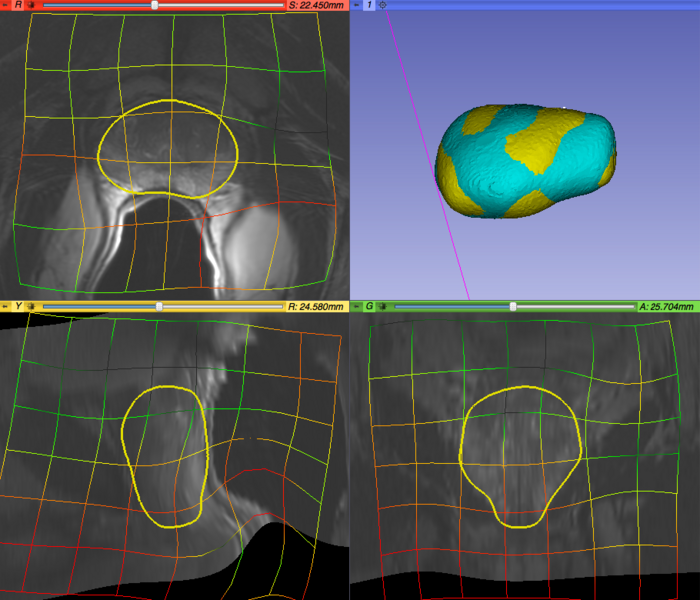
\includegraphics[width=10cm]{1_intro/img/MapBasedRegistration.png}
      \caption{Example of registration for MR images}
    \end{figure}

    他にも、臓器などの動き追跡のために用いられることがある。
    例えば、Fuら\cite{fu2011motion}はヒト下腿部のMR画像から、運動の追跡とひずみマップを作成した。
    また、Raghavendraら\cite{chandrashekara2003construction}はPCAも組み合わせ、心臓の運動を追跡するモデルを構築した。
    \begin{figure}[ht]
      \centering
      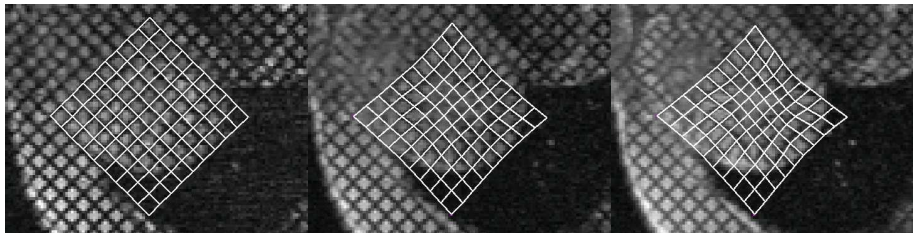
\includegraphics[width=14cm]{1_intro/img/heart_registration.png}
      \caption{A virtual tag grid used in registration for motion tracking of mid-ventricular short-axis slices\cite{chandrashekara2003construction}.}
    \end{figure}

    また、レジストレーションは放射線治療にも用いられている\cite{velec2011effect}。
    呼吸運動と線量蓄積の影響を変形画像レジストレーションを用いることで検討することが可能となり、正確なレジストレーションが可能となることにより、腫瘍および正常組織の線量の変化を定量化することができる。

    上記の通り、画像レジストレーション技術の発展に寄与することは医療の質や効率の向上だけでなく、医師の負担軽減にも繋がるため、非常に重要である。

\subsection{画像モダリティ}
    医療画像には様々なモダリティが存在する。
    医療分野においてモダリティとは、医療機器の種類やタイプを指す言葉であり、代表的なモダリティにはMRIやX線などが挙げられる。
    このモダリティのうち、一種類のみを用いてレジストレーションを行う場合、それをモノモーダルレジストレーション(monomodal registration)と呼ぶ。

    モノモーダルレジストレーションと異なり、2つまたはそれ以上の複数モダリティを対象に行われるレジストレーションはマルチモーダルレジストレーション(multimodal registration)と呼ばれる。
    多くの場合、異なる2つのモダリティから得られる画像は、補完的な性質を持つ。
    先程例に上げたMR-TRUSは、解像度とリアルタイム性を2つのモダリティによって補完し合っている。

    今日、モノモーダルレジストレーションの多くは高い精度で自動化され、実際に臨床でも利用され始めている。
    しかし、マルチモーダルレジストレーションにおいては、利用することの利点は明らかであるにも関わらず、診断臨床の現場ではほとんど行われていない\cite{viergever2016survey}。

\subsection{問題点}
    治療法の選択および治療計画の術前段階でのマルチモーダルレジストレーションは普及しているものの、自動化の研究は進んでいない。
    これには様々な理由が存在しているが、主な理由は以下に挙げる3点である。

    \subsubsection{レジストレーション対象および手法の多様性}
        自動レジストレーションの主な問題の一つに、その種類の豊富さが挙げられる。
        本項では、いくつかの例を挙げてその複雑性について論ずる。
    \begin{description}
        \item[次元数]\mbox{}\\
            まず、空間的な次元のバリエーションである。
            医療画像には2D平面だけでなく、3Dのボクセルを扱う場合がある。
            つまり、医療画像レジストレーションでは、少なくとも2D同士、2D-3D、3D 同士のレジストレーションの3種類が存在する。
            2-D-2-Dレジストレーションは、パラメータの数とデータ量の両方の複雑さがはるかに少ないので、多くの場合、3-D-3-Dの場合よりも簡単かつ迅速にレジストレーションすることが可能である。
            2-D-2-Dレジストレーションは、パラメータの数とデータ量が非常に少ないため、多くの場合、3-D-3-Dの場合よりも簡単かつ迅速にレジストレーションを行うことが可能である。
    
            また、空間的次元とは異なり、時系列を表す意味での次元が考慮される場合がある。
            例えば小児における骨の成長モニタリング\cite{saeed1998magnetic}などでは時系列的に同一患者の画像を比較することが求められる。
            さらに、このような時系列的な比較では空間的次元と同様にその間隔によってレジストレーションの難易度が変化する。
            高頻度で撮像を行えばレジストレーションはより容易になるが、逆に撮像の間隔が長い、または変化が早い場合にはレジストレーションの難易度は高くなる。
            

        \item[モダリティ]\mbox{}\\
            モダリティの多さも、レジストレーションの複雑性を増す原因となる。
            画像モダリティは、2つのカテゴリーに大別することができる。
            \begin{figure}[ht]
              \centering
              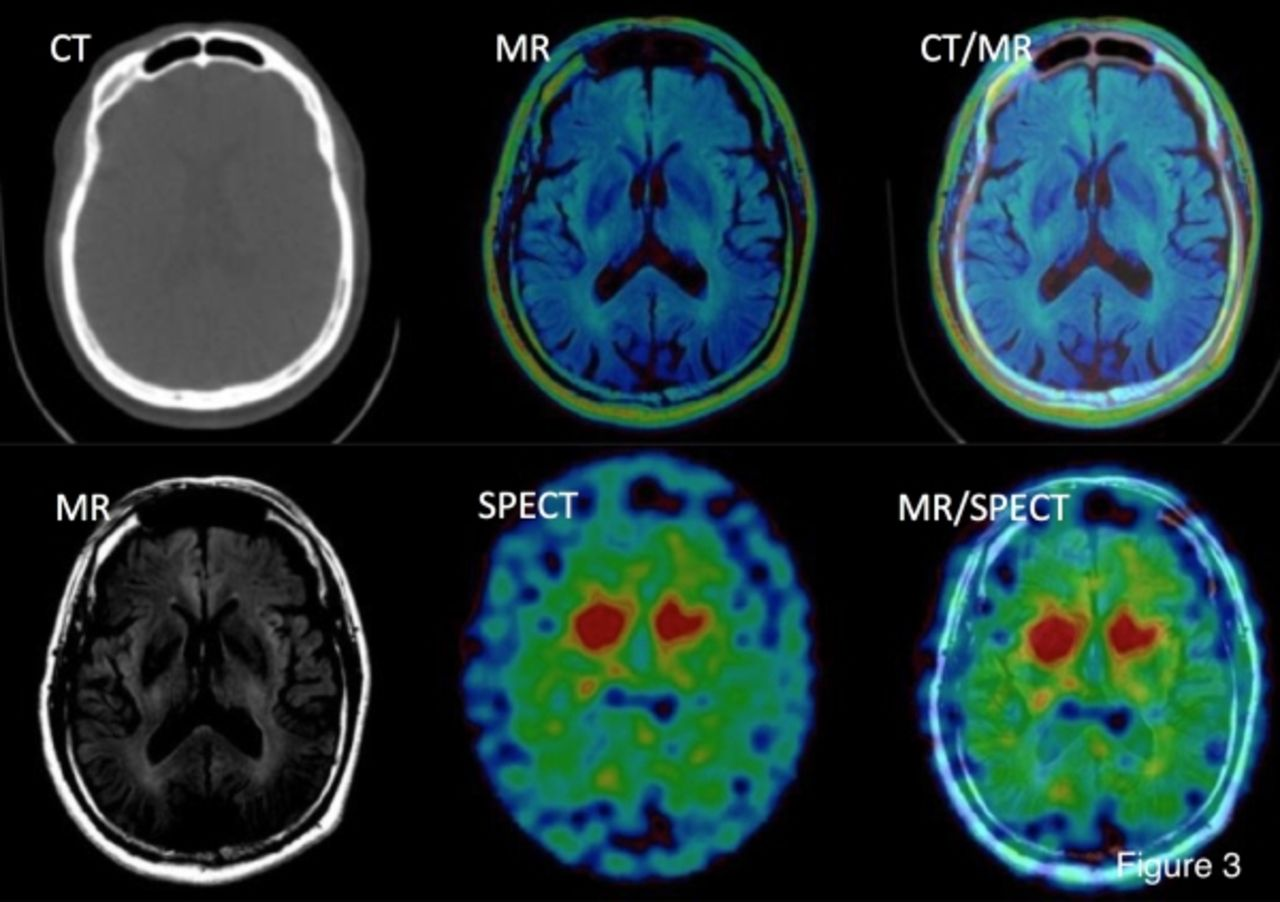
\includegraphics[width=12cm]{1_intro/img/MRCTSPECT.jpg}
              \caption{Brain cross-section images in various modality\cite{hara2016spect}.}
            \end{figure}
            一つは解剖学的モダリティであり、CT(Computed Tomography)、MRI(Magnetic Resonance Imaging)、X-ray、US(Ultrasound)などが存在し、その中でも、MRIなどはT1, T2などの細かい分類が存在する\cite{maintz1998survey}。
            もう一つは機能的モダリティであり、このモダリティは代謝に関する情報を主に描画する。
            例えばSPECT(single photon emission CT:単光子放出型コンピュータ断層撮影法)や、PET(Positron Emission Tomography : 陽電子放出断層撮影法)、fMRI(functional magnetic resonance imaging)などが挙げられる。
            他にも脳波などのような空間的に疎な技術も機能的画像技術と呼ぶことが可能であるが、一部を除きいた機能的モダリティの画像のほとんどが、レジストレーションには活用されない。
    
            このように、画像モダリティは非常に多様であり、またそれぞれのモダリティで特性が異なるため、すべてのモダリティで同時に動作する手法を開発することは困難を極める。
            さらに、異なるモダリティ同士のレジストレーションを行う、マルチモーダルレジストレーションの場合には、2つの画像を比較することすら困難であり、レジストレーションの難易度は飛躍的に高くなる。
            このようにモダリティの差異がレジストレーションにもたらす複雑性は特筆すべきものであるが、その程度は様々である。
            例えば、MR画像におけるT1,T2画像の差と、MR-US画像の差では、後者の差が前者と比べて非常に大きいことがわかる。
    
            また、モダリティの違いがもたらす複雑性は画像の外観だけに留まらない。
            撮像している機材が異なるということは、撮像する機器ごとに、撮像範囲、撮像するタイミング、患者の姿勢などが異なることになる。
            撮像範囲が異なる場合、比べる画像ごとに写っている臓器の数が異なることになる。
            また、撮像するタイミングが異なることによって、膀胱などの時間によって大きさが変化するような臓器への対応が困難になる。
            さらに、MRIやCTのように、体軸に沿って一定間隔ずつの画像しか撮像不可能な場合、完全に同じ断面を撮像することは困難である。
            加えて、患者の姿勢によって臓器の相対位置や断面方向に差が生じる可能性も考えられる。

        \item[変形手法]\mbox{}\\
            変形手法の多さも、レジストレーションの複雑性を増す原因となる。
            画像の変形手法には様々な方法が存在する。
            まず、変形対象の画像をパッチに分けてそれぞれを変形するパッチベースの手法と、画像全体を変形する手法に大別される。
            そして、具体的な変形手法として剛体変換、アフィン変換、透視変換、そして非線形変換と、4つの手法が存在する。
            \begin{figure}[ht]
              \centering
              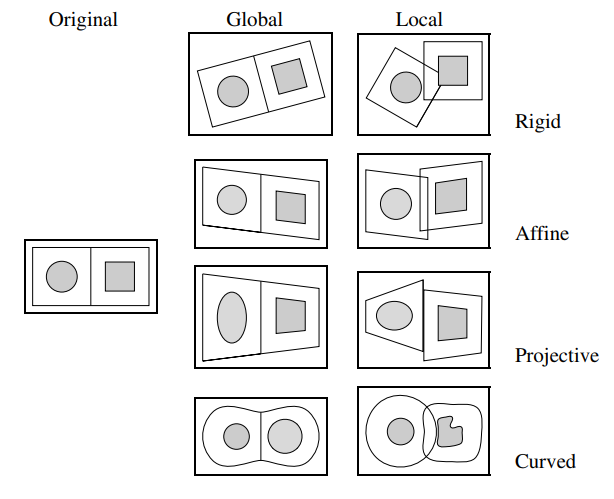
\includegraphics[width=10cm]{1_intro/img/2Dtransformations.png}
              \caption{Examples of 2-D transformations\cite{maintz1998survey}.}
            \end{figure}
    
            中でも非線形変換の方法は多岐に渡り、数式で一般的に表現することはない。
            非線形変換を用いた画像変形方法の一例としては、TPS(Thin Plate Spline)変換などが存在する。
            また、画像レジストレーションでも特にDIR(Deformable image registration)においては、displacement vector field (DVF)を用いた画像の変換が行われることが多い。
            これは非線形変換の一つであり、移動画像の各画素を対象画像の対応する画素位置に移動させるための変位ベクトル場(DVF)を生成することにより、移動画像を対象画像に合わせて変形させる技術である。
            
            以上のような多様な画像変形手法の中から、各研究が様々な手法を採用しており、定量的評価を行うのは困難を極めている。
            また、現在臨床現場に導入されているほとんどが最も簡単な剛体変換のみを採用している\cite{viergever2016survey}。
    \end{description}


    \subsubsection{データの欠如}
        データの欠如に関しても医療画像レジストレーションの自動化を妨げる大きな要因の一つである。
        % ref 2016 a survey of medical image registrations -under review
        医療画像レジストレーションに関するデータセット整備の必要性は度々指摘されており、深層学習が自動画像レジストレーションの研究に広く利用されるようになって以降、その傾向は顕著である。
        % ref deep learning in medical image registration: a review
        
        例えば、
    
    \subsubsection{検証の困難さ}
        医用画像レジストレーションの精度評価は非常に複雑で複雑である。
        この原因はこれまでに述べた2つの
        % ref 1998 survey of medical image registrations
        % ref 2016 a survey of medical image registrations -under review

\subsection{主な手法}
    画像レジストレーションの手法は,様々な角度から分類が可能である\cite{maintz1998survey}。
    例えば、画像レジストレーションを行うために患者の身体にマーカーを埋め込む侵襲的な手法\cite{lunsford2012modern, van1995automatic}と、そうでない手法で大別することが可能である。
    他には、レジストレーションの基準に何を用いるか(ランドマーク基準\cite{evans1996correlative, uenohara1995vision}、セグメンテーション基準\cite{zhao1993registration, andersson1995method}、ボクセル値基準)によって大別することも可能である。
    しかし、現在ではほとんどのレジストレーション操作が非侵襲的で、画像の比較にはボクセル(またはピクセル)を利用するようになった。

    現在用いられている主な手法は2つに大別される。
    類似度を最大化するように変形を繰り返す反復的手法と、変形パラメータを直接導出するパラメータ推定手法である。
    本節ではこの2つの分類に沿って、いくつかの医療画像レジストレーション手法を示す。
    
    \begin{figure}[ht]
      \centering
      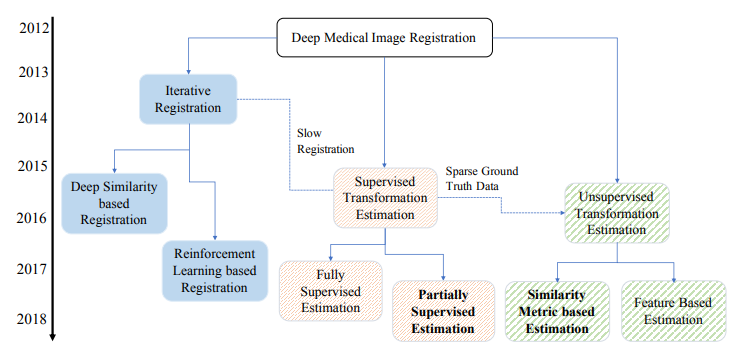
\includegraphics[width=14cm]{1_intro/img/classification_of_method.png}
      \caption{An overview of deep learning based medical image registration broken down by approach type. The popular research directions are written in bold.\cite{haskins2020deep}.}
    \end{figure}
    
    \subsubsection{反復的手法}
    
    \subsubsection{教師あり学習}
    
    \subsubsection{半教師あり学習}
    
    \subsubsection{教師なし学習}
    
    \subsubsection{敵対的学習}

    % TODO
    % 画像レジストレーションの主な手法
    % 反復的手法
    % パラメータ推定法
    % 医療画像レジストレーションの問題点
    % データの欠如
    % 検証の困難さ

\section{ドメイン適応}
    % TODO
    % ドメイン適応の分類
    % ドメイン適応の医療応用
    % 医療画像レジストレーションにおけるドメイン適応活用の現状
    \subsection{分類}
\subsection{医療応用}
\subsection{医療画像レジストレーションにおけるドメイン適応活用の現状}

\section{研究目的}
    % TODO
    \subsection{既存技術の問題点}

\subsection{課題設定}
    モダリティ間の外観差は入力データ分布の差であると捉えることができる.
    ドメイン適応(Domain Adaptation, DA)は入力データの分布の差に対処するための技術であり,医療画像においてはMultimodal Segmentationなどのタスクに応用されている.
    Multimodal Registrationに対してDAを用いる手法はいくつか存在するものの,Single Step Registrationに適用されている例は非常に少ない.

\subsection{貢献}
    本論文では、DAを用いることで,Registrationの教師データを用いることなくMultimodal Registrationが可能なモデルを訓練する手法を提案する.
    本論文で我々は自然画像で訓練されたRegistration modelの性能が、DAを用いることによってどのように変化するかを観察することにより,DAの医療画像Registrationへ応用可能性を示す.

\section{論文構成}
    この論文は次のように構成される.
    第1章は序論であり,本研究の背景並びにその目的について述べた.
    第2章は本研究の位置付けを明らかにするものであり,関連する研究について述べる.
    第3章はドメインの違いを確認する操作および、ドメイン適応を利用しない場合におけるマルチモーダル画像レジストレーションに関する実験の結果と考察について述べる.
    第4章では提案手法によるドメイン適応およびマルチモーダル画像レジストレーションの結果と考察について述べる.
    第5章では本研究に対する結論を述べる.

% 3.提案手法
\chapter{提案手法}
\thispagestyle{fancy} %ヘッダー・フッターの設定
卒業するために修士論文を書くのがよいと思います。

% 4.実験
\chapter{実験}
\thispagestyle{fancy} %ヘッダー・フッターの設定
面倒なのでやらなかった

% 5.考察
\chapter{考察}
\thispagestyle{fancy} %ヘッダー・フッターの設定
よくわからん


% 2.関連研究
\chapter{関連研究}
\thispagestyle{fancy} %ヘッダー・フッターの設定

%% 「。」を「.」にしたり、「、」を「,」にしたりするのは後で置換で一括でやります。

画像のレジストレーション手法は主に2つのモダリティ間の画像の類似度評価の技術と画像を変形させる技術に基づいて構成されている.
ここでは類似度評価手法および変換手法について主に使われている手法を述べてから, 具体的なレジストレーション手法について確認する.
また, 具体的な手法については特に医療画像に使用される技術について言及する.

\section{マルチモーダルレジストレーション}

%% 「。」を「.」にしたり、「、」を「,」にしたりするのは後で置換で一括でやります。

医療画像レジストレーションの中でも、モダリティを超えて画像の整合性を考慮するマルチモーダルレジストレーションは非常に難易度が高く、盛んに研究が行われているにも関わらず、未だに精度の高いレジストレーションは実現していない。
画像レジストレーションの精度は深層学習を用いることによって精度および速度が飛躍的に向上したものの、マルチモーダルレジストレーションに関しては

\subsection{古典的手法}

\subsection{類似度を用いた手法}

\subsection{強化学習を用いた手法}

\subsection{教師あり学習を用いた手法}

\subsection{半教師あり学習を用いた手法}

\subsection{教師なし学習を用いた手法}
 
\section{転移学習}
% DONE

%% 「。」を「.」にしたり、「、」を「,」にしたりするのは後で置換で一括でやります。

転移学習やドメイン適応は、あるタスクで学習したことを別のタスクの汎化能力向上に役立てようとする状況を指す言葉である。
マルチタスク学習との決定的な差は、マルチタスク学習がソースタスクとターゲットタスクを同時に学習するのに対して、転移学習はターゲットタスクを最も重要視する点にある。
深層学習を用いた医療画像処理において、学習データの欠如は非常に重要な問題であり、転移学習やドメイン適応を利用した少数データで十分に汎化したモデルを得る研究が非常に重要な課題になっている。    
前節までにおいて紹介してきた機械学習モデルの前提として、訓練データとテストデータは同様の分布であるという暗黙の了解がある。
例えば、カメラで撮影したRGB画像を入力として想定した、犬種判別モデルに赤外画像を入力しても良い精度は得られない。
また、上記のモデルに同じRGB画像を入力したとしても、猫の画像を入力しても無意味な結果が得られるだけである。
このように、多くの機械学習モデルは非常に厳しい前提条件の元にうまく機能するが、大抵の場合にはこの前提条件は適用されない。
しかし、仮に犬種判別のモデルの知識が猫種判別の知識に利用できる場合、犬種判別モデル作成に利用していたデータよりも少数のデータで猫種判別モデルを作成することが可能になる可能性がある。

このように、多量のラベリング作業によるコストおよび労力緩和のために、転移学習は非常に良い選択肢となりうる。
深層学習モデルの転移学習では、一般にImageNet用に設計された標準的なモデルが使用される。
これは特に視覚的なカテゴリ(画像に関するタスク)に限定されるが、視覚的なカテゴリではエッジや形などの概念、幾何学的変化による影響や、証明の変化などの特徴が共通であり、ImageNetで訓練されたモデルこれらを抽出可能なパラメータはすでに所持していると言える。
故に、出力に近い部分を学習することにより、様々なタスクへの応用が可能となる。

医療画像ではImageNetで訓練されたモデルに対して医療用画像で微調整を行い、胸部X線画像の解釈\cite{majkowska2020chest}、アルツハイマー病の早期発見\cite{ding2019deep}、目の疾患の特定\cite{varadarajan2018deep}などに使用している例がある。

\subsection{転移学習の定義}
    転移学習は様々な文献で多様な定義が行われている\cite{pan2009survey, zhu2011heterogeneous, shao2014transfer, zhang2017transfer}。
    転移学習やドメイン適用に関する概念は比較的新しく、まだ決まっていないことに加えて、本論文で扱うドメイン適応の説明のためには詳細な分類は不要であることから、ドメイン適用の位置づけを理解するために最低限必要である、最も基本的な分類\cite{pan2009survey}に関して述べる。
    
    まず、最も基本的な定義を理解するためには「ドメイン」および「タスク」の概念を定義する必要がある。
    ドメインとは、データ空間のことであり、ある特定の確率分布$P(X)$に従って分布しているデータ$X=\{x_1,x_2,...,x_n\}\in X$で張られる特徴量空間Xのことを指す。
    そして、タスクとはあるドメイン$D=\{X,P(X)\}$が与えられた際のラベル$Y=\{y_1,y_2,...,y_n\}\in Y$および、Xから学習可能な関数$f(\cdot )$から構成され、$T=\{Y,f(\cdot)\}$で表される。
    このとき、$X$および$Y$の要素は互いに対応している。
    
    そして、転移学習を考える際に最も重要なものが、ドメインの差異である。
    元となる知識があるドメインのことをソースドメインとして$D_S$と表し、転移先であるドメインをターゲットドメインとして$D_T$として表す。
    
    この条件の元での転移学習の定義は以下のようになる\cite{pan2009survey}。
    \begin{quote}
        ソースドメイン$D_S$と学習タスク$T_S$、ターゲットドメイン$D_T$と学習タスク$T_T$が与えられた場合、転移学習は$D_S \neq D_T$または$T_S \neq T_T$である$D_S$および$T_S$の知識を用いて、$D_T$における予測関数$f_T(\cdot)$の学習を改善することを目的としたもの。
    \end{quote}

\subsection{転移学習の分類}
    前項で示した転移学習の定義では、転移学習は$D_S \neq D_T$または$T_S \neq T_T$である場合を想定しているため、転移学習は様々なケースに分類することが可能である。
    転移学習の様々なケースは、データの特性に注目することで1)帰納的転移学習、2)伝達転移学習、3)教師なし転移学習の3種類に分類することが可能である。
    \begin{enumerate}
        \item 帰納的転移学習(Inductive Transfer Learning)\\
            帰納的転移学習は、転移学習の中でも特に$T_S \neq T_T$であるものを指す。この枠組みで更に特徴的なのは$T_S$および$T_T$がどちらも利用可能であることである。
            さらに、これらの中でも$D_S$かつが$D_T$のデータが豊富である場合、マルチタスク学習と呼ばれ、$D_T$のみデータが豊富である場合には半教師あり学習(自己教師あり学習, self-supervised learning)と呼ばれる。
        \item 伝達転移学習(Transductive Transfer Learning)\\
            伝達転移学習は、転移学習の中でも特に$D_S \neq D_T$であるものを指す。この学習ではソースドメインに多くのラベルが存在する一方、ターゲットドメインに十分な数のラベルが存在しない。
        \item 教師なし転移学習(Unsupervised Transfer Learning)\\
            教師なし転移学習は、帰納的転移学習と同様に$T_S \neq T_T$である場合を想定しているが、それぞれのタスクが独立せずに関連しているケースで用いる。
            この枠組みで更に特徴的なのはソースドメインおよびターゲットドメインのどちらでも十分なラベルデータが存在しないことである。
            故に、教師なし転移学習では次元削減やクラスタリングによって学習タスクを解くことが求められる。
    \end{enumerate}
    上記の転移学習の設定及び関連領域に関する分類を以下の表\ref{ClassificationOfTL}にまとめた

    \begin{table}[ht]
    \caption{Classification of Transfer Learning Settings and Related Domains\cite{pan2009survey}.}
    \resizebox{\textwidth}{!}{%
    \begin{tabular}{|l|l|l|l|}
    \hline
    Transfer Learning Settings                   & Related Areas            & Source Domain Label & Target Domain Label \\ \hline
    \multirow{2}{*}{Inductive Transfer Learning} & Multi-task Learning      & Available           & Available           \\ \cline{2-4} 
                                                 & Self-supervised Learning & Unavailable         & Available           \\ \hline
    Transductive Transfer Learning & \begin{tabular}[c]{@{}l@{}}Domain Adaptation, Sample \\ Selection Bias, Co-variate Shift\end{tabular} & Available & Unavailable \\ \hline
    Unsupervised Transfer Learning               &                          & Unavailable         & Unavailable         \\ \hline
    \end{tabular}%
    }
    \label{ClassificationOfTL}
    \end{table}

\subsection{転移学習のアプローチ}
    転移学習にはモデルの知識を転移させるために様々なアプローチが存在する。
    このアプローチ方法は、転移対象によって分類が可能である。
    以下では、転移学習を転移対象とその手法に基づいて転移学習を4つに分類する。
    \begin{enumerate}
        \item Instance-Transfer\\
            Instance-Transferの関心領域はデータ自体であり、ソースドメインのデータをターゲットドメインで利用するために、ソースドメインのデータを重み付けする手法である。
        \item Feature-representation-transfer\\
            Feature-representation-transferの関心領域はモデルのパラメータであり、ソースおよびターゲットのドメイン自体の差や、それぞれのドメインでの分類誤差を最小化する特徴量を見つける、または学習する手法である。
        \item Parameter-transfer\\
            Parameter-transferの関心領域はモデルのパラメータであり、ソースドメインで作成したモデルおよびターゲットモデルで作成したモデルにおける、パラメータの共通点を発見することによって、どちらのドメインでも用いることの可能なパラメータを作成するような手法である。
        \item Relational-knowledge-transfer\\
            Relational-knowledge-transferの関心領域は抽出後の特徴量であり、同一のモデルによって抽出されたそれぞれのドメインでの特徴量の対応付けを行い、知識のマッピングを行う手法である。
    \end{enumerate}

\subsection{医療画像応用における問題点}
    前項で触れたように転移学習は深層学習の医療画像応用において広範に利用されている。
    しかし、転移学習の正確な効果はまだ十分に理解されていない。
    医療画像だけでなく、特定のタスクに限定的に用いられるモデルに対して、ImageNetで訓練されたモデルの重みを転移学習に用いるのは意味がない場合が多い。
    特に医療画像では、ImageNetでは画像の主題を問われているのに対し、画像の特定の部分のみが関心対象であったり、データセットの規模や画像のスケールの隔たりなど、様々な差異が存在する。
    そのため、医療画像では転移学習によりパフォーマンスが大幅に向上することはなく、事前学習を適用しなかった単純なモデルも同等の精度を発揮することが示されているケースも報告されている\cite{raghu2019transfusion}。

\section{ドメイン適応}
% TODO
% ドメイン適応のアプローチ
% 医療画像におけるドメイン適応
% 本論文におけるドメイン適応(提案手法の方に回す?)

%% 「。」を「.」にしたり、「、」を「,」にしたりするのは後で置換で一括でやります。

ドメイン適応は、大量のラベルデータの不足に対処するための新たな学習手法であり、転移学習の特殊なケースとして位置づけられる。
前節の定義に従うと、ドメイン適応は転移学習の中でも特に$D_S \neq D_T$であるものを指す。

本節では、Wanら\cite{wang2018deep}の論文による分類を元に、特に深層学習に注目して、ドメイン適応の定義と分類を示した後に、医療画像レジストレーションタスクがドメイン適応においてどのように分類されるのかを示す。

\subsection{ドメイン適応の分類}
    深層学習のような手法を用いない場合、ドメイン適応のアルゴリズムは2つに大別できる。
    1つ目は、ソースドメインでのラベルをターゲットドメインで利用するために、ソースドメインのデータ自体に重み付けをするような転移学習(Instance Transfer)である。
    2つ目は、ソースドメインおよびターゲットドメインの差や、モデル誤差を軽減する特徴量を見つけるような転移学習(Feature representation transfer)である。

    深層学習におけるドメイン適応を考慮する際に、このドメインの違いについての形態は、 それぞれのドメインが同質であるかどうかによってさらに2つに分類することが可能である。
    先述したように、ドメイン適応は転移学習の特殊なケースとして位置づけられ、$D_S \neq D_T$の場合を想定している。
    しかし、この定義ではこの差異がデータの分布によるものなのか、特徴空間の差異のことなのかは明確にされていない。
    そこで、、Wanら\cite{wang2018deep}はデータ分布のみが異なり、特徴空間は同一である場合をHomogeneous DA、特徴空間自体が異なる場合をHeterogeneous DAとして分類している。
    
    Heterogeneous DAは特徴空間自体が異なる場合であるが、取り扱うメディア自体が同じ場合と異なる場合でさらに2種類に分けることができる。
    取り扱うメディア自体が同じ(例:画像対画像)場合は、例えばデータ取得に利用したデバイスの差(可視光、近赤外、奥行き付映像など)や、画像スタイルの差異(絵と写真など)などのケースが考えられ、取り扱うメディア自体が異なる場合(例:画像対言語)には、メディアが同じ場合よりもドメインの差異が非常に大きくなる。

    深層学習モデルにおけるドメイン適応を考慮する際には、基本的にInstance Transferのような手法について議論されることは少ない。
    深層学習モデルをどのように設計すれば異なるドメインの表現を獲得することが可能かを議論することが大半であり、本論文ではこのような汎用的な特徴表現を学習することを前提としてドメイン適応を分類する。
    具体的には、データの種類によって学習の方法は「教師あり学習」「半教師あり学習」「教師なし学習」の3つに大別することができる。
    つまり、深層学習のOne-Stepドメイン適応は、ドメインの質に関して2通り、学習方法に関して3通りの分岐が存在し、合計で6つに分類することが可能であることが分かる(図\ref{category_of_DA})。
    
    \begin{figure}[ht]
      \centering
      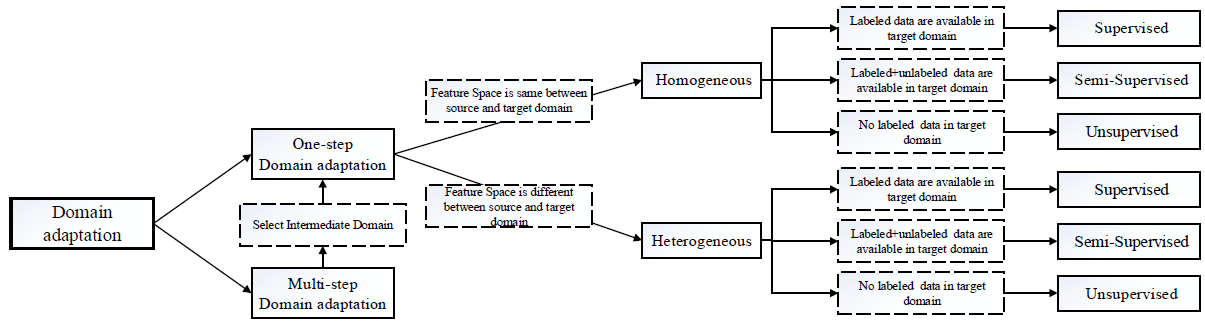
\includegraphics[width=\linewidth]{2_related_works/img/category_of_DA.png}
      \caption{An overview of different settings of domain adaptation\cite{wang2018deep}.}
      \label{category_of_DA}
    \end{figure}

    また、ドメインの特性が互いにあまりにも違う場合には、稀に中間のドメインを経由してドメイン適応を行う例(Multi-Step Domain Adaptation)も存在するが、本論文ではそのような例は扱わない。
    

\subsection{ドメイン適応のアプローチ}
    深層学習モデルをドメイン適応させるために、様々なアプローチが考案されている。
    これらのアプローチは大きく分けて3つに分類することができる\cite{csurka2017domain}。
    \subsubsection{Discrepancy base}
        discrepancyベースのアプローチは、教師データを用いて深層学習モデルを最適化する中でドメインシフトに対応する手法である。
        
        用いる損失関数や何を基準にするかによってさらに細分化されるが、多くが通常の深層学習モデルの訓練と同様に訓練が可能である。
        
        
        
        
    \subsubsection{Adversarial base}
        Adversarialベースのアプローチは、GANを用いてドメインの混合を促す手法である。
    \subsubsection{Reconstruction base}
        Reconstructionベースのアプローチは、補助的なタスクとして画像再構成を課すことにより、特徴量の普遍性を確保することを目指す手法である。
    
\subsection{医療画像におけるドメイン適応}
    医療画像におけるドメイン適応は、


\subsection{本論文におけるドメイン適応}
    本論文では、転移学習の中でも特にドメイン適応に焦点を当てる。
    すなわち、想定するのは$D_S \neq D_T$である状態であり、転移対象に関してはモデルのパラメータを想定する。
    %これはMR-CTなど、画像モダリティの違いを指す。
    基本的に後に述べる敵対的手法\cite{goodfellow2014generative}を用いてモデルを訓練することによりパラメータのドメイン適応を行い、2つのドメインに共通して利用できるモデルを作成することを目標とする。
    つまり、転移学習の枠組みにおいて、本研究はFeature-representation-transferを用いて伝達転移学習を行うことに焦点を当てている。
    しかし、ラベルの有無などの点で細かい定義から多少外れていることに注意されたい。
    次節ではドメイン適応について詳しく述べる。


% 6.結論
\chapter{結論および今後の展望}
\thispagestyle{fancy} %ヘッダー・フッターの設定

\section{結論}
卒業させて

% 謝辞
% !TEX root = ../main.tex
\chapter{謝辞}
\thispagestyle{fancy} %ヘッダー・フッターの設定
めちゃありがとう


%添付資料
% !TEX root = ../main.tex

\appendix
\thispagestyle{fancy} %ヘッダー・フッターの設定

%%%%%%%%%%%%%%%%%%%%%%%%%%%%%%%%%
\chapter{深層学習の基礎}

\section{機械学習}
    機械学習とは,特定課題に対してコンピュータが効率よく動作するようなパターンを見つけるアルゴリズムまたは統計モデルの研究分野であり,人工知能研究の一つとして数えられる.
    機械学習はルールベースのアルゴリズムなどとは異なり,アルゴリズムが人間に判断基準を明示されることなく,判断基準をデータから見つけるような動作をするアルゴリズムのことである.
    機械学習の父とも呼ばれるアーサー・サミュエルによれば,機械学習は
    \begin{quote}
        Field of study that gives computers the ability to learn without being explicitly programmed
        
        明示的にプログラムしなくても学習する能力をコンピュータに与える研究分野
    \end{quote}
    であると定義されている\cite{samuel1959some}.さらに,具体的には経験$(E)$に基づいて,精度$(P)$がタスク$(T)$に対して最適化されていくようなアルゴリズムのことを指すとしている.
    
    機械学習は,例えばN個の訓練集合(training set)${\bm{x}_1, \bm{x}_2, \bm{x}_3, ... , \bm{x}_N}$が与えられたとき,それに対応する目標ベクトル(target vector)${\bm{t}_1, \bm{t}_2, \bm{t}_3, ... , \bm{t}_N}$と,訓練集合を用いて予測したベクトル${\bm{y}_1, \bm{y}_2, \bm{y}_3, ... , \bm{y}_N}$の誤差が最小になるような関数$f_w(x)$を得るような操作である.
    このとき,誤差の計算で用いる関数を誤差関数(Error function),コスト関数(Cost function)または損失関数(Loss function)と呼ぶ.
    一度訓練集合と目標ベクトルで訓練されたモデルは,異なるデータ集合に対しても適用可能である.
    例えば,数字認識のモデルでは数字が描かれている画像(訓練集合)と画像に対応する数字(目標ベクトル)が与えられ,分類モデル$y(x)$が得られた場合,訓練集合に無い画像に対してもモデルは数字の予測を行うことが可能である.
    このような訓練集合と異なる新たな事例に対して予測を行う能力のことを汎化(generalization)と呼ぶ.
    以上のような枠組みは教師あり学習と呼ばれ,機械学習の中でも最も良く用いられる手法の一つである.
    
    機械学習は大きく分けて教師あり学習,教師なし学習,強化学習の3つに大別することができる.
    教師あり学習は先程のように訓練集合と目標ベクトルが与えられ,誤算関数を最小化,または汎化するようなモデルを得るような操作のことである.
    これと比べ,教師なし学習はその名の通り目標ベクトルを持たない.
    教師なし学習では,訓練集合の中で似通ったデータをまとめるクラスタリングや,データの次元圧縮などが行われ,それに伴ってデータの視覚化(Visualization)などに活用されることが多い.
    最後の強化学習は,試行錯誤を通じて「価値を最大化するような行動」を学習する手法である.
    これは教師あり学習と同じ目的のように思われるが,教師あり学習とは目標ベクトルが詳細に定義されていない点で異なる.
    強化学習の場合には最終的な目標(例えばゲームに勝利する,電力効率を上げるなど)のみが与えられるタスクや,あらかじめ詳細な目標が分からない(または,取得が困難である)ようなタスクに対してより良い振る舞いをさせることが目標となる.
    
    機械学習の様々な種類について触れたが,単純に機械学習と呼ばれる場合には教師あり学習のことを指す場合が多い.
    教師あり学習には大きく分けて分類と回帰という2つのタスクが存在している.
    教師あり学習におけるこの2つのタスクタイプの顕著な違いは,その出力形式である.
    分類タスクでは出力値は離散値をとり,不連続である.
    これは例えば明日の天気を予測したり,画像から花の種類を予測したりといったタスクが該当する.
    一方,回帰タスクは連続値をとる.
    これには,例えば明日の気温の予測や,数々の条件から家の値段を推測するようなタスクが該当する.
    
    また,この2つのタスクが複合することもありうる.
    近年深層学習の貢献によって大きな発展を遂げた物体検出が顕著な例である.
    物体検出では物体の位置がどこであるかを回帰し,物体な何であるかを分類する.
    また,分類時の確率を出力することは回帰であると捉えることも可能である.
    
    本節では,実際に教師あり学習の枠組みの中の機械学習のアルゴリズムを複数示し,次節に示す深層学習の理解の助けとする.

\subsection{線形回帰}
    線形回帰は最も一般的な機械学習のアルゴリズムであり,このアルゴリズムは名前の通り回帰タスクを実行する.
    このアルゴリズムは訓練集合および目標ベクトルの組み合わせ${\bm{x},\bm{y}}$が与えられたとき,その誤差を最小化するようなパラメータ$\bm{w}$を持つ関数$f_w(\cdot )$を求めるアルゴリズムである.
    
    以下では,簡単のため訓練集合および目標ベクトルをそれぞれ1次元データとして考え,$w_0$(バイアス項)を無視する.
    すると,最適化対象の式(hypothesis)$h(x)$はと以下のように表すことができる.
    \begin{equation}
        h_w(x) = w_0 + w_1 x
    \end{equation}
    よって,あるデータ$(x, y)$についての誤差は以下のように表すことができる.
    \begin{equation}
        Error(w_1) = h_w\left(x\right)-y
    \end{equation}
    訓練集合${x^{(1)}, x^{(2)}, x^{(3)}, ... , x^{(N)}}$および対応する目標値${y^{(1)}, y^{(2)}, y^{(3)}, ... , y^{(4)}}$が与えられ,それぞれに対する誤差の合計値を最小化することを考える.
    つまり,線形回帰における損失関数は以下のようになる.
    \begin{equation}
        L(w_1) = \frac{1}{2N}\sum_{i=1}^{N}\left(h_w (x^{(i)})-y^{(i)}\right)^2
    \end{equation}
    ここで,総和および$1/N$で各誤差の平均をとっていることがわかる.($1/2$が乗算されていることについては後述する.)
    また,単純な誤差の平均ではなく,誤差の二乗を取っていることに注意する.
    これは誤差における符号の影響をなくすために用いられる.
    平均二乗誤差(Mean Square Error)は回帰においてしばしば用いられる損失関数の一つで,二乗ではなく誤差の絶対値を用いる手法を平均絶対値誤差(Mean Absolute Error)と呼ぶ.
    
    \begin{figure}[t]
        \begin{center}
            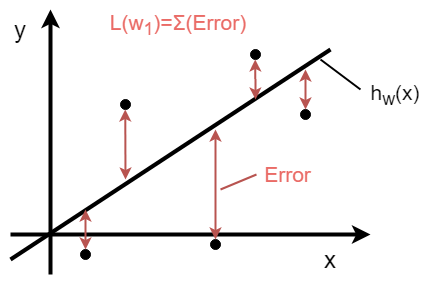
\includegraphics[width=8.0cm]{./8_appendix/img/error}
            \caption{Simplified diagram of the loss function in linear regression.}
            \label{2_linerregression_loss}
        \end{center}
    \end{figure}
    
    さて,次にこの損失関数を最小化する方法を考える.
    $h_w(x)=w_1 x$より,先程の損失関数は以下のように表すことができる.
    \begin{equation}
        L(w_1) = \frac{1}{2N}\sum_{i=1}^{N}\left(w_1 x^{(i)} - y^{(i)}\right)^2
    \end{equation}
    上記の式において,$x^{(i)}$ および $y^{(i)}$は既知の値であることから,$L(w_1)$は$w_1$に関する下に凸の2次関数となることが分かる.
    つまり,線形回帰において最小二乗誤差を最小化することは,損失関数の微分値が0になる値を求めることと等価である.
    
    さて,先程は2つの大きな仮定を用いて数式を単純化した.
    一つは訓練集合が1次元であるという仮定.
    もう一つは$w_0$(バイアス項)が0であるという仮定である.
    実際には訓練集合は多変数である場合がほとんどであり,バイアス項を考慮しないと精度の良いモデルは得られない.
    以降では多変数の場合の線形回帰について見ていく.
    
    多変数を考える線形回帰は特に重回帰分析と呼ばれ,最適化対象の式(hypothesis)$h(x)$は,以下のように表すことができる.
    \begin{equation}
        h_{\bm{w}}(\bm{x}) = w_0・1 + w_1 x_1 + w_2 x_2 + ...  + w_d x_d = \bm{w}^T\bm{x}
    \end{equation}
    このような多項式は線形モデルとも呼ばれる.
    線形モデルに関して,損失関数は同様に以下のように定義される.
    ここで$\bm{x}=(x_1, x_2, x_3, ... , x_d)$であることに注意する.
    \begin{equation}
        L(\bm{w}) = \frac{1}{2N}\sum_{i=1}^{N}\left(h_{\bm{w}}(\bm{x}^{(i)})-y^{(i)}\right)^2
        \label{linerregression_loss_equation}
    \end{equation}
    先程,線形回帰においては最小二乗誤差を最小化することは,損失関数の微分値が0になる値を求めることと等価であると述べた.
    これは重回帰分析においても同様であり,パラメータ$\bm{w}$は以下の式を解くことによって導出できる.
    \begin{equation}
        \frac{\partial L(\boldsymbol{w})}{\partial \boldsymbol{w}}=\frac{\partial}{\partial \boldsymbol{w}} \frac{1}{2N} \sum_{i=1}^{N}\left(h_{\boldsymbol{w}}(\boldsymbol{x}^{(\boldsymbol{i})})-y_{n}\right)^{2}=\mathbf{0}
    \end{equation}
    ここで,訓練集合について,以下で定義される行列のことを慣習として計画行列(デザイン行列)と呼び,$\Phi$で表す.
    
    \begin{equation}
        \bm{\Phi}=\left(
            \begin{array}{ccccc}
                1 & x^{(1)}_1 & x^{(1)}_2 & \cdots & x^{(1)}_d \\
                1 & x^{(2)}_1 & x^{(2)}_2 & \cdots & x^{(2)}_d \\
                1 & x^{(3)}_1 & x^{(3)}_2 & \cdots & x^{(3)}_d \\
                \vdots & \vdots & \vdots & \ddots & \vdots \\
                1 & x^{(N)}_1 & x^{(N)}_2 & \cdots & x^{(N)}_d
            \end{array}\right)
    \end{equation}
    
    これを用いて先程の損失関数を表すと,以下のようになる.
    \begin{eqnarray}
        L(\bm{w}) &=& \frac{1}{2N}\left( \bm{w\Phi} - \bm{y} \right)^2\  =\  \frac{1}{2N}\left( \bm{w\Phi} - \bm{y} \right)^T \left( \bm{w\Phi} - \bm{y} \right)\\
        &=& \frac{1}{2N}\left( \bm{w}^T\bm{\Phi}^T - \bm{y}^T \right) \left( \bm{w\Phi} - \bm{y} \right)\\
        &=& \frac{1}{2}\left(\bm{w}^T \bm{\Phi} \boldsymbol{w}-\boldsymbol{w}^T \bm{\Phi}^T \boldsymbol{y}-\boldsymbol{y}^T \bm{\Phi} \boldsymbol{w}+\boldsymbol{y}^T \boldsymbol{y}\right)\\
        &=& \frac{1}{2}\left(\bm{w}^T \bm{\Phi} \boldsymbol{w}-2\boldsymbol{w}^T \bm{\Phi}^T \boldsymbol{y}+\boldsymbol{y}^T \boldsymbol{y}\right)
    \end{eqnarray}
    つまり,損失関数の微分は以下のように求まる.
    ここで,先程乗算した$1/2$が微分値を簡素な値にしていることに注意する.
    \begin{eqnarray}
        \frac{\partial L(\boldsymbol{w})}{\partial \boldsymbol{w}} 
        &=&\frac{\partial}{\partial \boldsymbol{w}} \frac{1}{2}\left(\boldsymbol{w}^T \bm{\Phi}^T \bm{\Phi} \boldsymbol{w}-2 \boldsymbol{w}^T \bm{\Phi}^T \boldsymbol{y}+\boldsymbol{y}^T \boldsymbol{y}\right) \\
        &=&\frac{1}{2} \frac{\partial}{\partial \boldsymbol{w}} \boldsymbol{w}^T \bm{\Phi}^T \bm{\Phi} \boldsymbol{w}-\frac{1}{2} \frac{\partial}{\partial \boldsymbol{w}} 2 \boldsymbol{w}^T \bm{\Phi}^T \boldsymbol{y}+\frac{1}{2} \frac{\partial}{\partial \boldsymbol{w}} \boldsymbol{y}^T \boldsymbol{y} \\
        &=&\frac{1}{2}\left(\bm{\Phi}^T \bm{\Phi}+\left(\bm{\Phi}^T \bm{\Phi}\right)^T\right) \boldsymbol{w}-\bm{\Phi}^T \boldsymbol{y} \\
        &=&\bm{\Phi}^T \bm{\Phi} \boldsymbol{w}-\bm{\Phi}^T \boldsymbol{y}\\
        &=&\bm{\Phi}^T \left( \bm{\Phi} \boldsymbol{w} - \boldsymbol{y} \right)
    \end{eqnarray}
    以上より,線形回帰における最適解は以下のように解析的に求めることができる.
    \begin{eqnarray}
        \bm{\Phi}^{\mathrm{T}}(\bm{\Phi} \boldsymbol{w}-\boldsymbol{y})&=&\mathbf{0} \\
        \boldsymbol{w}&=&\left(\bm{\Phi}^T \bm{\Phi}\right)^{-1} \bm{\Phi}^T \boldsymbol{y}
    \end{eqnarray}
    
    以上のように線形回帰においてパラメータ$\bm{w}$を求める方程式を正規方程式と呼ぶ.
    正規方程式は計画行列の逆行列を計算することで一度に計算を終わらせることが可能である.
    一方,この方法は計算量が$O(n^3)$で増加するため,大規模なデータに関しては計算時間がかかりすぎるというデメリットがある.
    そのため,大規模なデータに対しては後述する最急降下法という最適化手法が用いられる.
    
    また,線形回帰はデータ間の線形的な関係しか捉えることができないが,非線形な関係を捉えるためにデータのn乗を考慮した多項式に関する回帰を行う場合がある.
    これは多項式回帰と呼ばれる手法だが,データがn乗になっているだけで,本質的に重回帰分析と等価である.

\subsection{正則化}
    線形回帰を含む様々な機械学習アルゴリズムは,汎化せずに訓練集合にのみ良い予測を与えるモデルを生む可能性がある.
    このように訓練データに適応しすぎた結果,汎化性能が悪化する現象を過学習と呼ぶ.
    
    具体的に多項式回帰に関して考える.
    $y=ax^2+bx+c$で表されるような疑似データを生成する.
    このデータ${x,y}$の関係は通常の場合不明であることが多い.
    つまり,通常は多項式回帰を行う際にはn次元の多項式を用意して,パラメータを導出することが多い.
    すると,以下の図\ref{2_overfitting}のように過学習が起きる可能性が考えられる.
    ここで,図の左側よりも右側の関数のほうが訓練誤差は小さいと考えられる.
    しかし,xが十分に大きい,または小さいような,訓練データに無いデータが入力された場合の汎化誤差は右側の関数の方が遥かに大きくなると考えられる.

    \begin{figure}[t]
        \begin{center}
            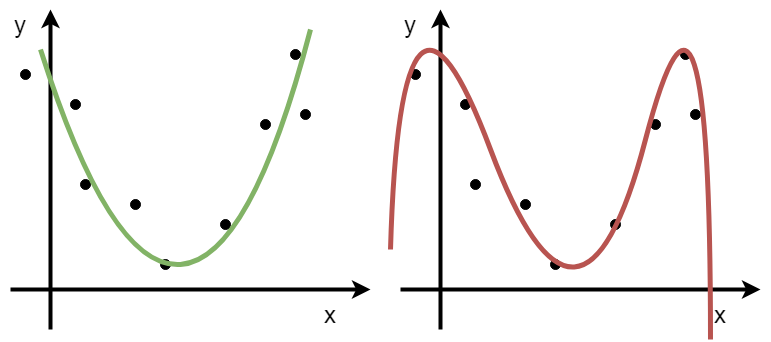
\includegraphics[width=10.0cm]{./8_appendix/img/regularization}
            \caption{Example of model behavior when overfitting occurs.}
            \label{2_overfitting}
        \end{center}
    \end{figure}
    例えば先程の例で以下の多項式を考えていた場合,$w_4$の値が大きくなったと考えられる.
    \begin{equation}
        h_{\bm{w}}(\bm{x}) = w_0 x^0 + w_1 x^1 + w_2 x^2 + w_3 x^3 + w_4 x^4 + w_5 x^5
    \end{equation}
    このように,特定のパラメータが大きくなりすぎることによって汎化性能が低下することを防ぐためにはモデルの正則化が重要である.
    
    モデルの正則化の発想は非常に単純で,損失関数にパラメータの値自体を組み込むことで,パラメータのスケールが必要以上に大きくなることを防ぐ.
    損失関数の中でも,特にこのような項を正則化項と呼ぶ.
    また,機械学習の枠組みではこのような正則化項の選び方を特に荷重減衰(weight decay)と呼ぶ.
    この正則化項を考慮した線形回帰の損失関数は以下のように表すことができる.
    \begin{equation}
        L(\bm{w}) = \frac{1}{2N}\sum_{i=1}^{N}\left(h_{\bm{w}}(\bm{x}^{(i)})-y^{(i)}\right)^2-\alpha \sum^M_{j=0}w_{j}^2
    \end{equation}
    ここで,$\alpha$は正則化の強さを決定するハイパーパラメータである.
    また,導出は省くが正規化項を考慮した正規方程式の解は以下のようになる.
    \begin{equation}
        \bm{w}=\left( \bm{\Phi}^T\bm{\Phi}+\alpha \bm{I} \right)^{-1}\bm{\Phi}^T\bm{y}
    \end{equation}
    また,上記の式では正則化項としてパラメータの二乗を用いているが,これは$|w_j|^q$として一般化できる.
    機械学習の枠組みではq=1のL1正則化,およびq=2のL2正則化がよく用いられる.
    統計学の分野においてはq=1のときを特にLassoと呼ぶ\cite{tibshirani1996regression}.
    このL1正則化(またはLasso)は,$\alpha$が十分に大きいときにいくつかのパラメータが0となる,疎な解が得られる.
    
\subsection{ロジスティック回帰}
    線形回帰は回帰を行うモデルであったのに対して,ロジスティック回帰は分類を行うモデルである.
    
    まず,分類問題の目標ベクトルについて考える.
    簡単のためにここでは二値分類を扱う.
    二値分類の場合,目標値は0または1になる.
    説明変数xのある値について0と1を分類する線形モデルは例えば,図\ref{2_classification}中における緑の線を描くようなモデルが考えられる.
    \begin{figure}[ht]
        \begin{center}
            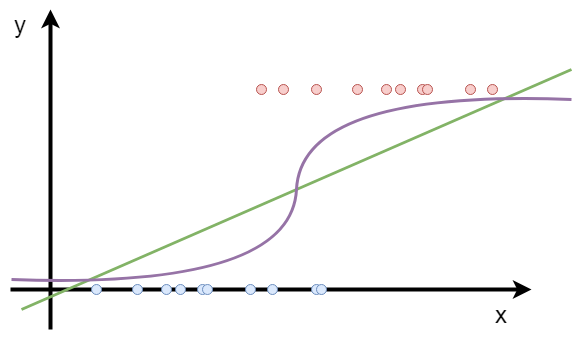
\includegraphics[width=10.0cm]{./8_appendix/img/classification}
            \caption{Schematic diagram of the classification model.}
            \label{2_classification}
        \end{center}
    \end{figure}
    しかし,このモデルはxを十分大きく(または十分小さく)した場合に1を超える(または0を下回る)ために,実用的とは言えない.
    以上から,出力が$0\leq h_w(x) \leq 1$となるようなモデル$h_w(x)$を考えるべきである.
    ここで以下の式で示されるsidmoid関数を導入する.
    \begin{equation}
        g(x)=\frac{1}{1+e^{-x}}
    \end{equation}
    この関数はロジスティック関数とも呼ばれ,図\ref{2_sigmoid}のような形状をしている.
    \begin{figure}[ht]
        \begin{center}
            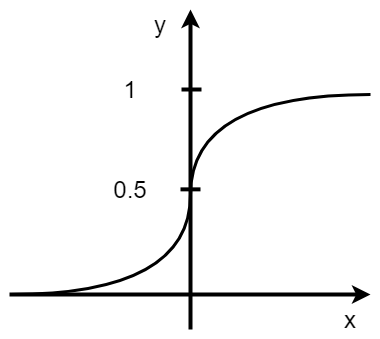
\includegraphics[width=7.0cm]{./8_appendix/img/sigmoid}
            \caption{Sigmoid function}
            \label{2_sigmoid}
        \end{center}
    \end{figure}
    
    線形回帰の出力にこのsigmoid関数を適用することにより,図\ref{2_classification}中における紫の線を描くようなモデルが得られる.
    ロジスティック回帰のモデルを線形モデルおよびsigmoid関数を利用して表現すると以下のような式になる.
    \begin{equation}
        h_{\bm{w}}(\bm{x}) = g\left(\bm{w}^T\bm{x}\right)=\frac{1}{1+e^{-\bm{w}^T\bm{x}}}
    \end{equation}
    つまり,閾値を0.5とすると,線形モデルの出力$\bm{w}^T\bm{x}$が正の値を取るときy=1と分類され,負の値を取るときy=0と分類される.
    以上から,入力空間はy=0となる境界により分割されることがわかる.
    このときの境界を決定境界(decision boundary),分割された領域を決定領域(decision region)と呼ぶ.
    簡単な例として,${w_,w_1,w_2}={-3,1,1}$とした際の分類境界を図\ref{2_classification_example}に示す.
    決定領域の中でも線形の決定面によって分離可能なデータ集合を特に線形分離可能(linearly separable)という.
    このとき,図\ref{2_classification_example}に示したように,入力データを加工することにより非線形境界も学習できることも注意したい.
    \begin{figure}[ht]
        \begin{center}
            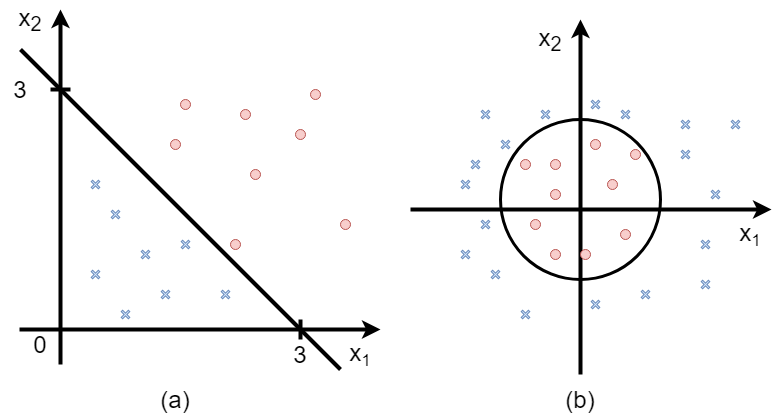
\includegraphics[width=12.0cm]{./8_appendix/img/classification_example}
            \caption{Classification boundary by logistic regression when the threshold is set to 0.5.\ (a)$x_1+x_2-3=0$\ (b)$x_1^2 + x_2^2-1=0$}
            \label{2_classification_example}
        \end{center}
    \end{figure}
    
    また,ロジスティック回帰におけるsigmoid関数のように,線形モデルに対して何かしらの変換を施す非線形関数のことを,機械学習分野では特に活性化関数(activation function)と呼ぶ.
    また,上記で見たように,活性化関数が非線形の場合にも,このモデルの決定境界は線形である.
    また,このようなsigmoid関数に限らない様々な非線形変換を線形モデルに施すことを想定した,ロジスティック回帰よりも一般化されたモデルのことを一般化線形モデル(generalized linear model\cite{mccullagh81nelder})と呼ぶ.

    ロジスティック回帰において決定境界を決定する$\bm{w}$は,線形回帰と同様に損失関数を最小化することによって導出できる.
    線形回帰は二乗誤差を利用して損失関数を定義したが,ロジスティック回帰において最小二乗誤差を利用するのは不適である.
    式\ref{linerregression_loss_equation}で表される損失関数において,線形モデルの場合,$h_{\bm{w}}(\bm{x})$は線形である.
    しかし,sigmoid関数を利用しているロジスティック回帰モデルの場合には,$h_{\bm{w}}(\bm{x})$は非線形となる.
    つまり,損失関数$L(\bm{w})$は非凸関数となり,局所解が増加し,大域解を求めるのが困難になる.
    \begin{figure}[ht]
        \begin{center}
            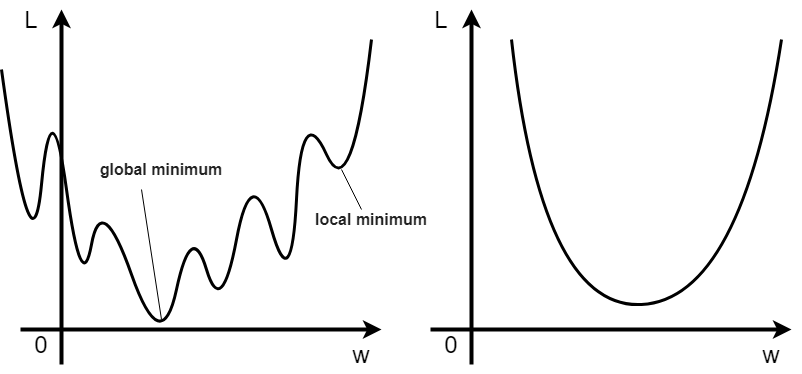
\includegraphics[width=12.0cm]{./8_appendix/img/global_minimum}
            \caption{Comparison of the solution space of the loss function by Mean Square Error when using linear and non-linear models.}
            \label{2_global_minimum}
        \end{center}
    \end{figure}
    
    そこで,分類タスクにおいては,以下のような損失関数を定義する.
    \begin{eqnarray}
        L\left(h_{\bm{w}}(\bm{x}), \bm{y}\right)=\left\{ \begin{array}{ll}
            -\log(h_{\bm{w}}(\bm{x})) & if\ y=1 \\
            -\log(1-h_{\bm{w}}(\bm{x})) & if\ y=0 \\
            \end{array} \right.
    \end{eqnarray}
    この損失関数は交差エントロピー誤差関数(cross-entropy error function)として広く知られている.
    この交差エントロピーを用いることによって誤差関数が収束することは,負の対数を図示すると直感的に理解できる.
    \begin{figure}[ht]
        \begin{center}
            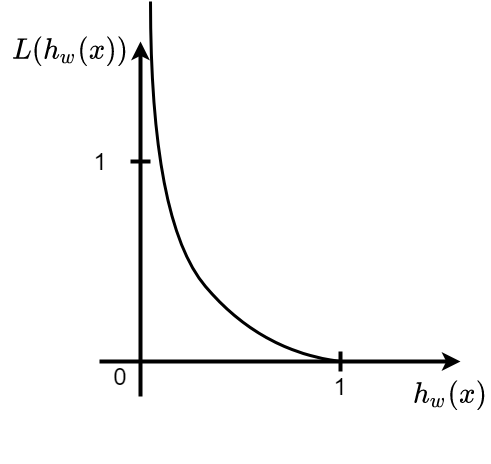
\includegraphics[width=7.0cm]{./8_appendix/img/log_negative}
            \caption{Loss function defined as a negative logarithm. (The domain is 0 <h (x) <1)}
        \end{center}
    \end{figure}
    
    この損失関数は計算機上で簡便に計算するために以下のようにも定義される.
    \begin{equation}
        L\left(h_{\bm{w}}(\bm{x}), \bm{y}\right)= -y \log(h_{\bm{w}}(\bm{x})) -(1-y)\log(1-h_{\bm{w}}(\bm{x}))
    \end{equation}
    つまり,各データの損失を考慮したときの一般化された損失関数は以下のようになる.
    \begin{equation}
        L(\boldsymbol{w}) = \frac{1}{N}\sum^N_{i=1}\left[-y^{(i)} \log(h_{\bm{w}}(\bm{x}^{(i)})) +(1-y^{(i)})\log(1-h_{\bm{w}}(\bm{x}^{(i)}))\right]
    \end{equation}
    
    さて,線形回帰と同様にロジスティック回帰についても微分値を求める.
    シグモイド関数の微分値は式\ref{sigmoid_eq}表すことができることに注意すると,損失関数の微分値は式\ref{logistic_loss_differential}で表すことができる.
    \begin{equation}
        \frac{\partial g(\boldsymbol{x})}{\partial \boldsymbol{x}} = g(x) (1-g(x))
        \label{sigmoid_eq}
    \end{equation}
    \begin{eqnarray}
        \frac{\partial L(\boldsymbol{w})}{\partial \boldsymbol{w}_j} 
        &=& \frac{1}{N}\sum^N_{i=1}\left[-y^{(i)} \frac{\partial \bm{z}}{\partial \boldsymbol{w}_j}\frac{\partial }{\partial \boldsymbol{z}}\log(\bm{z}) + (1-y^{(i)})\frac{\partial \bm{z}}{\partial \boldsymbol{w}_j}\frac{\partial }{\partial \boldsymbol{z}}\log(1-\bm{z})\right]\\
        &=& \frac{1}{N}\sum^N_{i=1} \left[-y^{(i)} h_{\bm{w}}(\bm{x}^{(i)})(1-h_{\bm{w}}(\bm{x}^{(i)}))\frac{\bm{x}^{(i)}}{h_{\bm{w}}(\bm{x}^{(i)})} \right.\\ 
        &&  \left.+(1-y^{(i)})(\bm{x}^{(i)})(1-h_{\bm{w}}(\bm{x}^{(i)}))\frac{h_{\bm{w}}(\bm{x}^{(i)}))}{(1-h_{\bm{w}}(\bm{x}^{(i)}))}\right] \\
        &=& \frac{1}{N}\sum^N_{i=1}\left(h_{\bm{w}}(\bm{x}^{(i)})-\bm{y}^{(i)}\right)\bm{x}^{(i)}_j
        \label{logistic_loss_differential}
    \end{eqnarray}
    この式は線形回帰の二乗和誤差と同じであることが分かる.
    
    さて,ここまでで二値分類の場合を考えてきたが,多クラス分類にロジスティック回帰を適用するのは至って簡単である.
    各クラスごとに,一対多の分類を行えば良い.
    これは本質的に今まで行っていた分類と何ら変わりがない.
    \begin{figure}[ht]
        \begin{center}
            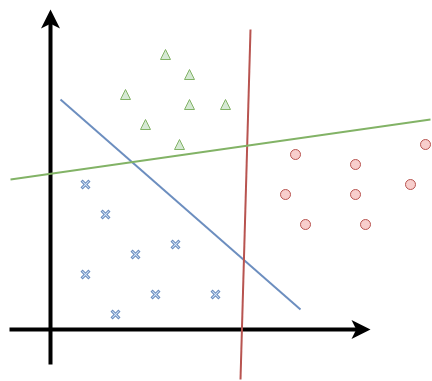
\includegraphics[width=8.0cm]{./8_appendix/img/one_vs_all}
            \caption{Overview of One-to-Many Classification.}
            \label{2_one_vs_all}
        \end{center}
    \end{figure}
    
    しかし,出力値の解釈には問題が生じる.
    ロジスティック回帰モデルは出力の範囲が$0\leq h_w(x) \leq 1$となるために,確率を出力するモデルとして考えることができる.
    つまり,ロジスティック回帰モデルの出力は$h_w(x)$は以下のような条件付き確率として表すことができる.
    \begin{equation}
        h_w(x)=P\left( y=k|x,w \right)
    \end{equation}
    ここで,kはクラスの値である.
    
    多クラス分類の際にそのまま一対多の分類を行った場合,各クラスの分類器が出力する値の合計は1を超える,または下回ることになる.
    そこで,各分類機の出力を正規化するために,ソフトマックス変換が用いられる.
    パラメータ$w$を持つ関数$h_w(x)$のクラス$k$に対する出力を$h^k_w(x)$とすると,ソフトマックス関数を用いて,各クラスに対する予測の条件付き確率は以下のように表すことができる.
    \begin{equation}
        P\left( y=k|x,w \right) = \rm{Softmax}(h^k_w(x)) = \frac{\exp{h^k_w(x)}}{\sum^K_{i=1}\exp{\left(h^i_w(x)\right)}}
    \end{equation}
    ここで,Kは合計のクラス数を表す.
    
    また,ロジスティック回帰の出力を確率値と捉えると,ロジスティック回帰は対数尤度を最大化するようにパラメータを学習していると捉えることができる.
    \begin{equation}
        \ln P=\sum_{n=1}^{N}\left\{y^{(n)} \ln \tilde{Y}\left(\mathbf{x}^{(n)} ; \mathbf{w}\right)+\left(1-y^{(n)}\right) \ln \left(1-\tilde{Y}\left(\mathbf{x}^{(n)} ; \mathbf{w}\right)\right)\right\}
    \end{equation}




\section{深層学習}
深層学習は2012年のImageNetチャレンジ\cite{ILSVRC15}でAlexNet\cite{krizhevsky2012imagenet}が大きな成功を収めて以来,急速に発展し,あらゆるタスクにおいて高度な能力を発揮している\cite{alom2018history}.
これは画像処理の分野では特に顕著で,医療画像処理も例外ではない\cite{litjens2017survey}.
しかし,深層学習に関する基礎的な考え方が成立したのは1940年代である\cite{Goodfellow-et-al-2016}.
そして,現在多く研究されているような畳み込みニューラルネットワーク(Convolutional Neural Network;CNN)\cite{lecun1998gradient}の基礎となっているネオコグニトロン\cite{fukushima1982neocognitron}が発表されたのは1982年であり,今日の深層学習技術を理解するにはそれらの簡単な歴史的経緯および理論的背景を学ぶことが重要である.

本節では前節で触れた機械学習の基礎となる線形回帰およびロジスティック回帰と深層学習の関連に触れつつ,深層学習の基礎的な考えを示す.

\subsection{多層パーセプトロン}
    人工ニューラルネットワーク(Artificial Neural Network;ANN)は生物学的学習の計算機モデルであり,脳の中で学習が行われている様子を模倣して,計算機のためのモデルに落とし込んだものである.
    パーセプトロンは最も単純なニューラルネットワークモデルであり,複数の信号を受け取り,一つの信号を出力するアルゴリズムである.
    出力されるのは信号を流す(1)か流さない(0)かの2値である.
    パーセプトロンは以下の数式\ref{neuron}で表される.
    ここで入力は$x$, 出力は$y$で表され, $\theta$は閾値とする.

    \begin{eqnarray}
        a&=&\sum_{j}w_{j}x_{j}+b \nonumber \\
        y&=&\left
                \{
                \begin{array}{ll}
                1 & (a\geq \theta) \\
                0 & (a<\theta) \\
                \end{array}
            \right.
        \label{neuron}
    \end{eqnarray}
    パーセプトロンの概要図を\ref{perceptron}に示した.
    \begin{figure}[ht]
      \centering
      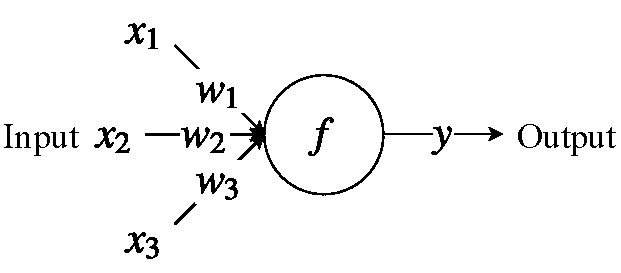
\includegraphics[width=10cm]{8_appendix/img/perceptron.pdf}
      \caption{Perceptron.}
      \label{perceptron}
    \end{figure}
    ここで,閾値(threshold)は,人工ニューロンにおける重み$w_{i}$と同様に学習によって変化するパラメータの一種であり,左辺に移し,バイアス$b$として置き換えると,次のようになる.
    \begin{align}
      y =   \begin{cases}
                0 \quad\text{if}\quad \sum_{j}w_{j}x_{j} + b \leq 0 \\
                1 \quad\text{if}\quad \sum_{j}w_{j}x_{j} + b > 0
            \end{cases}
    \end{align}
    このように,人工ニューロンの働きは,入力$x$に応じて値を出力する関数$f$として考えることができる.
    ここで,このパーセプトロンが前節における一般化線形モデルと同等であることに注意されたい.

    以上のようにパーセプトロンは線形分類器として利用ができる.
    つまり以下の図\ref{gate}中(a)(b)のように論理回路のAND素子やOR素子を実装することができる.
    パーセプトロンの出力部分を上記の式ではしきい値によって制御したが, この部分は一般化線形モデルにおける活性化関数を用いて実装できる.
    つまり,この場合には活性化関数としてステップ関数が用いられていると言える.
    通常,この活性化関数にはシグモイド関数やtanhなどの微分可能な関数が用いられる.
    微分可能な関数が用いられる理由については,後述の誤差逆伝播法を参照されたい.
    以下に,ニューラルネットワークに用いられる主な活性化関数を列挙する.
    
    \begin{itemize}
        \item 恒等写像関数
            \begin{equation}
                h(x)=x
            \end{equation}
        \item ステップ関数
            \begin{align}
              h(x)= \begin{cases}
                        1 \quad\text{if}\quad x \geq 0 \\
                        0 \quad\text{if}\quad x < 0
                    \end{cases}
            \end{align}
        \item sigmoid関数
            \begin{equation}
                h(x)=\frac{1}{1+e^{-\bm{w}^T\bm{x}}}
            \end{equation}
        \item tanh関数
            \begin{equation}
                h(x)=tanh(x)=\frac{\sinh(x)}{\cosh(x)}=\frac{e^x-e^{-x}}{e^x+e^{-x}}
            \end{equation}
        \item Rectified Linear Unit (ReLU)関数\cite{nair2010rectified}
            \begin{align}
              h(x)= \begin{cases}
                        x \quad\text{if}\quad x \geq 0 \\
                        0 \quad\text{if}\quad x < 0
                    \end{cases}
            \end{align}
        \item LeakyReLU関数\cite{maas2013rectifier}
            \begin{align}
              h(x)= \begin{cases}
                        x \quad\text{if}\quad x \geq 0 \\
                        ax \quad\text{if}\quad x < 0
                    \end{cases}
            \end{align}
        \item Softplus関数\cite{dugas2001incorporating}
            \begin{equation}
                h(x)=\log{(1+\exp(x))}
            \end{equation}
        \item Hardtanh関数
            \begin{align}
              h(x)= \begin{cases}
                        x \quad\text{if}\quad -1 \leq x \geq 1 \\
                        1 \quad\text{if}\quad x > 1 \\
                        -1 \quad\text{if}\quad x < -1
                    \end{cases}
            \end{align}
        \item Softmax関数
            \begin{equation}
                y_k = \frac{\exp{a_k}}{\sum^K_{i=1}\exp{\left(a_i\right)}}
            \end{equation}
    \end{itemize}

    さらにパーセプトロンを多層に重ねたものを多層パーセプトロンと呼び, NAND素子については図\ref{gate}中(c)のように3層パーセプトロンで実装できる.
    以上のように多層パーセプトロンは非線形な分類問題にも対応している.
    
    \begin{figure}[ht]
        \begin{center}
            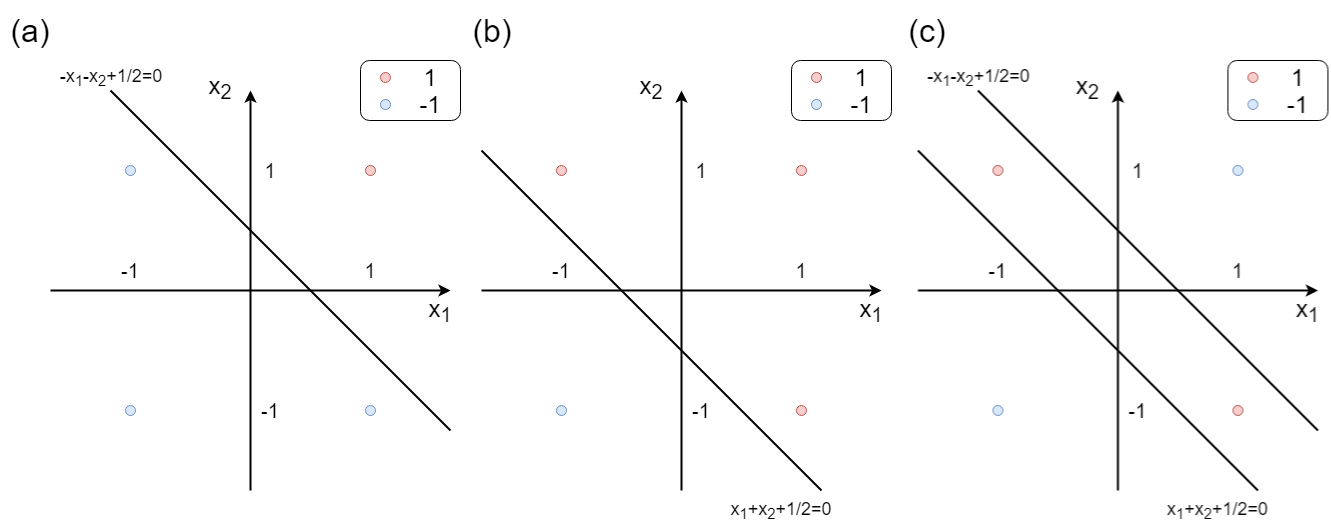
\includegraphics[width=16.0cm]{./8_appendix/img/gate.png}
            \caption{logic circuits implemented by formal neurons (a) AND gate (b)OR gate (c) NANDgate using a three-layer perceptron.}
            \label{gate}
        \end{center}
    \end{figure}
    
    この多層パーセプトロンを基礎とする人工ニューラルネットワークは,単純にニューラルネットワークと呼ばれることが多い.
    ニューラルネットワークにおいて,値の入力をする層を入力層,出力をする層を出力層という.
    そして,これら入力層と出力層の間に存在する多数の中間層を隠れ層という.
    図\ref{fig:mlperceptron}のようなニューラルネットワークでは,入力層から入力されたデータが中間層を経て出力層へと順番に計算,伝播していくため,順伝播型ニューラルネットワークと呼ばれる.

    \begin{figure}[ht]
        \begin{center}
            \centering
            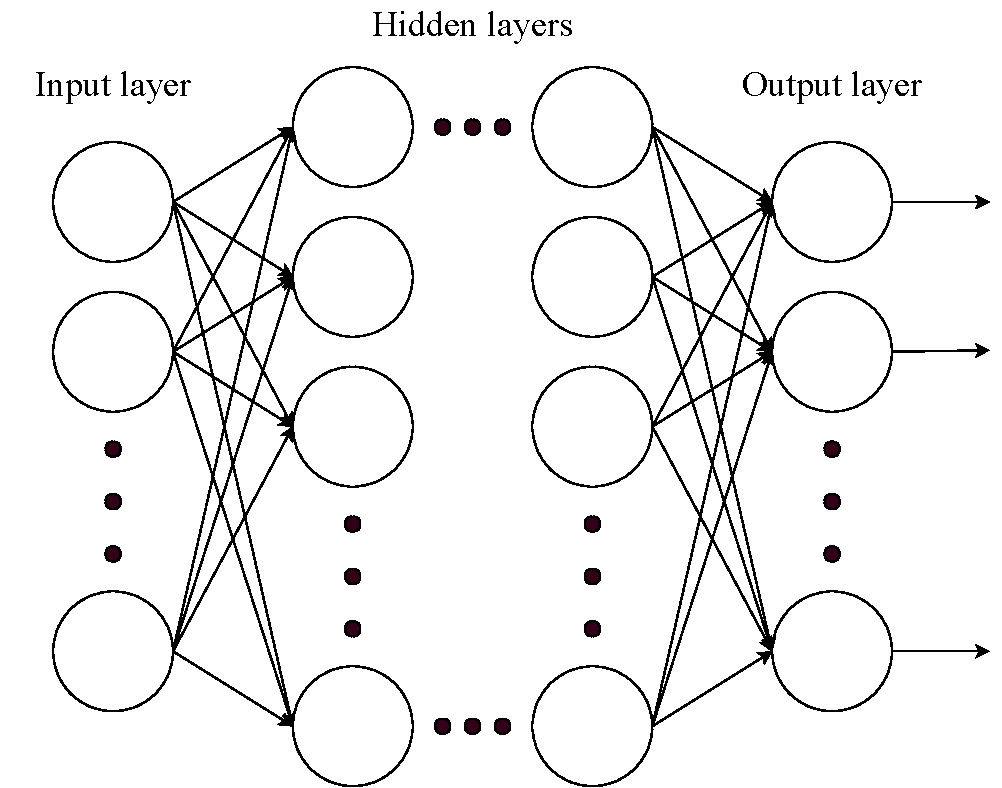
\includegraphics[width=10cm]{8_appendix/img/multi_layer_perceptron.pdf}
            \caption{Multi layer perceptron.}
            \label{fig:mlperceptron}
        \end{center}
    \end{figure}
    パーセプトロンの多層化により,様々な入力$x$と出力$y$の関係を同時に表すことができるようになった.
    例えば,Hornikら\cite{hornik1989multilayer}やCybenko\cite{cybenko1989approximation}らの万能近似定理(universal approximation theorem)によると,ネットワークが十分な数の隠れユニットを持つ場合,線形の出力層とシグモイド関数のような「押しつぶす」活性化関数をもつ隠れ層が少なくとも1つ含まれる順伝播型ネットワークは,どんなボレル可測関数でも任意の精度で近似できると述べられている.
    つまり,ノードを増やしていくと,ニューラルネットワークの表現力は上昇していき,学習データをほぼ完全に説明できるニューラルネットワークが実現できる.
    ただし,学習データを完全に説明できるモデルが実現した場合でも,そのモデルの汎化性能が必ずしも高いわけではないことに注意されたい.

\subsection{勾配に基づく最適化}
    このニューラルネットワークは,今まで示した通り,非常に高度な表現力を有する.
    しかし,このモデルのパラメータは線形回帰やロジスティック回帰のように解析的に求めることはできない.
    ニューラルネットワークの学習では,線形回帰やロジスティック回帰と同様に,モデルの指標として損失関数が定義され,損失関数を最小化することによって学習が行われる.
    ニューラルネットワークの場合,この損失関数の解空間が度重なる非線形変換によって非常に複雑になる(非凸となる).
    また,膨大な量のデータを学習することが多いため,一度にすべてのデータに対して計算が実行不可能であることなども問題である.
    
    そこでニューラルネットワークの訓練には,最急降下法\cite{cauchy1847methode}(または勾配降下法)がよく用いられる.
    この手法の発想は非常に単純である.
    最急降下法は,ある関数の一点に関して勾配(微分)を計算することにより,最も勾配が急である方向に向けてパラメータを動かす手法である.
    ここで,非常に単純化した最急降下法を用いたパラメータの更新式を以下に示す.
    \begin{equation}
        w^{(i+1)}=w^{(i)}-\eta\frac{\partial f_w}{\partial w^{(i)}}
    \end{equation}
    ここで$\eta$は学習率と呼ばれる,学習速度を調整するためのハイパーパラメータである.
    
    以上の単純な式を念頭におき,実際にどのように最急降下法が動作するかを詳しく見ていく.
    ニューラルネットワークに入力$\bm{x}^{\text{T}} = (x_{1}, x_{2}, x_{3})$を入力したときの出力が$\bm{y}^{\text{T}} = (y_{1}, y_{2})$であったとする.
    このとき目標とする出力を$\bm{t}^{\text{T}} = (t_{1}, t_{2})$とし,その誤差を$E(\bm{y}, \bm{t})$とする.このとき,ニューラルネットワークは誤差$E$を最小化する$\hat{\bm{y}}$を出力することを目的とし,学習が行われる.この条件は以下の式で表される.
    \begin{equation}
      \hat{\bm{y}} = \rm{argmin}_{\bm{y}}(E(\bm{y}, \bm{t}))
    \end{equation}
    ここで,$\hat{\bm{y}}$を解析的に求めることは困難であることは先程述べた.そこで,
    $\bm{y}$を微小量$\delta\bm{y}$だけ変化させた際の誤差$E(\bm{y}+\delta \bm{y}, \bm{t})$が$E(\bm{y}, \bm{t})$よりも小さくなる状態を考える.つまり,
    \begin{align}
      E (\bm{y} + \delta \bm{y}, \bm{t}) < E(\bm{y}, \bm{t}) 
      \label{eq:e_hikaku}
    \end{align}
    を満たすような$\delta\bm{y}$を求める.ここで,$E(\bm{y}+\delta \bm{y}, \bm{t})$はテイラー展開により次のように近似される.
    \begin{align}
      E(\bm{y}+\delta\bm{y}, t) &\approx E(\bm{y}, \bm{t}) + \frac{\partial E(\bm{y}, \bm{t})}{\partial \bm{y}} \delta \bm{y}
      \label{eq:e_taylor}
    \end{align}
    式\ref{eq:e_taylor}より,式\ref{eq:e_hikaku}を整理すると次式のようになる.
    \begin{align}
      E (\bm{y} + \delta \bm{y}, \bm{t}) \approx E(\bm{y}, \bm{t}) + \frac{\partial E(\bm{y}, \bm{t})}{\partial \bm{y}} \delta \bm{y} &< E (\bm{y}, \bm{t}) \nonumber \\
      E(\bm{y}, \bm{t}) + \frac{\partial E(\bm{y}, \bm{t})}{\partial \bm{y}} \delta \bm{y} &< E(\bm{y}, \bm{t}) \nonumber \\
      \therefore \frac{\partial E(\bm{y}, \bm{t})}{\partial \bm{y}} \delta \bm{y} &< 0
      \label{eq:e_back_jouken}
    \end{align}
    したがって,式\ref{eq:e_back_jouken}を満たす$\delta \bm{y}$を求めればよい.ここで,
    \begin{align}
      \delta \bm{y} &= -\bm{\eta} \frac{\partial E(\bm{y}, \bm{t})}{\partial \bm{y}}
    \end{align}
    とする.ただし,$\bm{\eta}$は正の微小量である.これを式\ref{eq:e_back_jouken}に代入すると次式のようになる.
    \begin{align}
      \frac{\partial E(\bm{y}, \bm{t})}{\partial \bm{y}} \left( - \bm{\eta} \frac{\partial E(\bm{y}, \bm{t})}{\partial \bm{y}} \right) &< 0  \nonumber \\
      - \bm{\eta} \left( \frac{\partial E(\bm{y}, \bm{t})}{\partial \bm{y}} \right)^{2} &< 0 
      \label{eq:e_back_final}
    \end{align}
    ここで,$\left( \frac{\partial E(\bm{y}, \bm{t})}{\partial \bm{y}} \right)^{2} \geq 0$ であるため,
    $\left( \frac{\partial E(\bm{y}, \bm{t})}{\partial \bm{y}} \right)^{2} \neq 0$の条件のもと,
    式\ref{eq:e_back_final}は成り立つ.また$\left( \frac{\partial E(\bm{y}, \bm{t})}{\partial \bm{y}} \right)^{2} = 0$のとき,$  E (\bm{y} + \delta \bm{y}, \bm{t}) = E(\bm{y}, \bm{t}) $となる.これは$\delta \bm{y}$の変化を与えても誤差$E$をより小さくすることが出来ない状態を表し,$\bm{y}$が最適解または局所解である状態を表す.
    よって誤差$E$をより小さくする,つまり式\ref{eq:e_hikaku}を満たすためには,$\bm{y}$を次のように更新できれば良い.
    \begin{align}
      \bm{y} \to \bm{y} + \delta \bm{y} = \bm{y} - \bm{\eta} \frac{\partial E(\bm{y}, \bm{t})}{\partial \bm{y}}
      \label{eq:e_y_result}
    \end{align}
    したがって,上記の式のようにニューラルネットワークの出力$\bm{y}$を更新できれば良いということが明らかになった.
    
    最急降下法ではすべてのデータに対して順伝播計算を行った後に勾配を求める.
    このような手法はバッチ勾配降下法と呼ぶ.
    しかし,計算機上の制約などによりすべてのデータを用いて勾配を計算することは現実的ではない.
    そのため,データの中からランダムに少数のデータを抽出し,そのデータで勾配を求める.
    特に,一度に1サンプルしか用いない手法を確率的勾配降下法,またはオンライン学習と呼ぶ.
    
    深層学習で主に用いられるのは上記2つの手法の中間的手法であり,使用する訓練データの数は複数だが,全てを用いるわけではない.
    このような少数のデータのまとまりをミニバッチと呼び,それ故にこれらの手法は確率的ミニバッチ勾配降下法や,単純に確率的勾配降下法と呼ばれる.
    今日では確率的勾配降下法という場合にはこちらを指していることが多い.
    
    ミニバッチに用いられる訓練データの数はバッチサイズと呼ばれ,バッチサイズによってモデルの訓練は以下のような性質を示す.
    \begin{itemize}
        \item バッチサイズが大きいと勾配推定が正確になる.(ただし,その改善度は線形以下となる)
        \item バッチサイズが大きいと計算効率が高い.(通常,計算機の効率の観点から2のべき乗の値が用いられる)
        \item バッチサイズが小さいと得られる勾配が毎回大きく異なってしまうため,学習がうまくいかない場合が多い
        \item バッチサイズが小さいと正則化の効果が得られる場合がある\cite{wilson2003general}
    \end{itemize}
    
    \subsubsection{悪条件}
    損失関数の解空間では,様々な悪条件が存在する.
    例えば,局所解はその最たる例である.
    ニューラルネットワークの損失関数は非凸であり,微分値が0になるような極小値を複数持つ場合がある.
    微分値が0になると学習が停滞するため,このような極小値が最小値と比べて高い値を持つのであれば問題である.
    
    他の悪条件としては鞍点が挙げられる.
    鞍点は(saddle point)とは,停留点(stationary points)のうち,極大値(local maximum)でも極小値(local minimum)でもない点のことであり,その一点において勾配が0になる.
    しかし,大抵の最適化手法は,この鞍点を回避することが知られており\cite{goodfellow2014qualitatively},実用上鞍点を回避することについて意識することは少ない.
    \begin{figure}[ht]
        \begin{center}
            \centering
            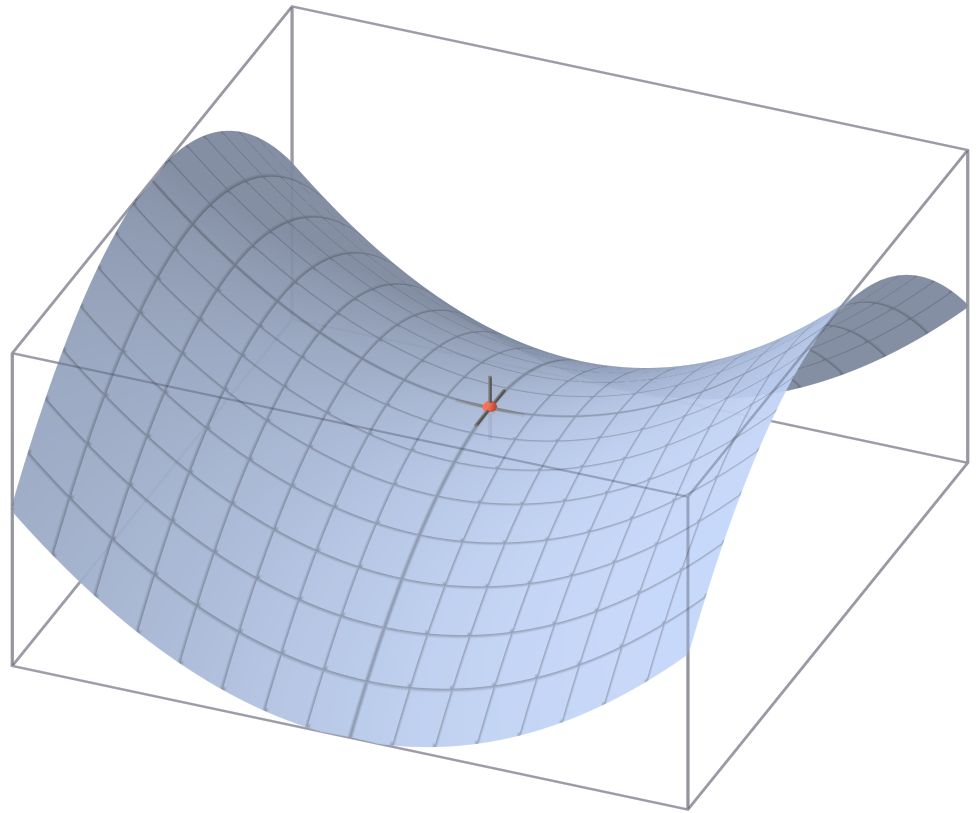
\includegraphics[width=10cm]{8_appendix/img/Saddle_point}
            \caption{Example of a saddle point.}
        \end{center}
    \end{figure}
    
    鞍点の他にも勾配がほとんど得られず学習が停滞する悪条件があり,これはプラトーと呼ばれる.
    プラトーでは損失関数の解空間が非常に平坦になるため,勾配がほとんど得られない.
    
    逆に,勾配が非常に急激な崖となっている場合も存在し,この崖の部分で損失関数は非常に大きな勾配を得る.
    すると,崖の逆方向に大きくパラメータが更新されてしまい,適切な学習が行われない場合がある.
    \begin{figure}[ht]
        \begin{center}
            \centering
            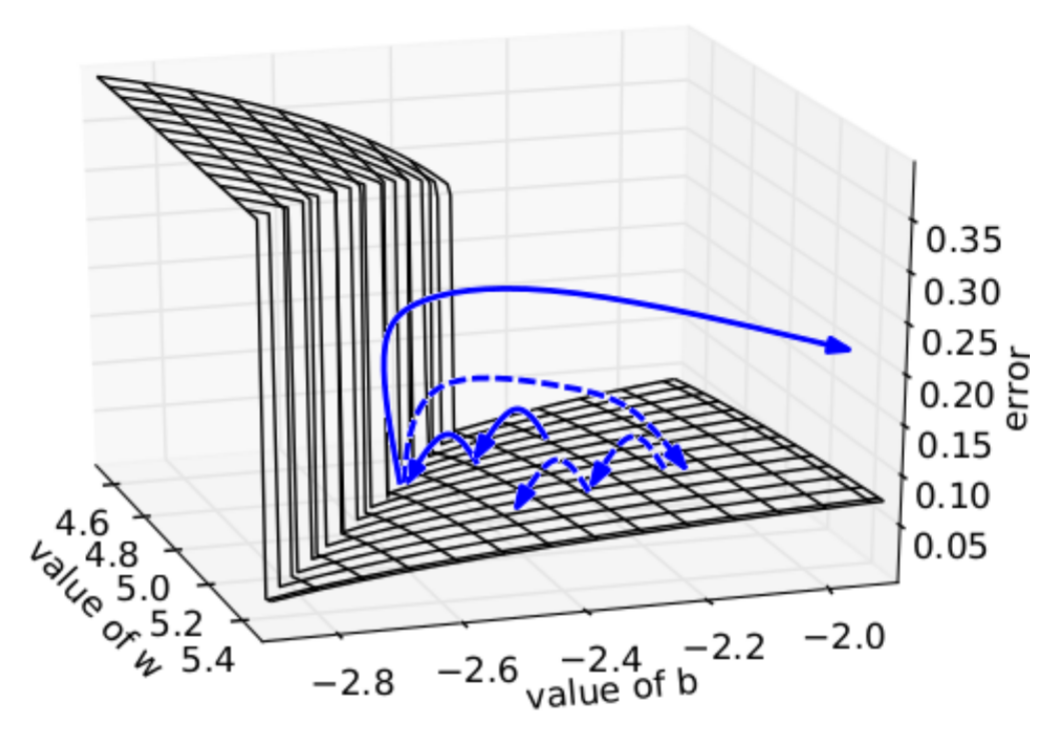
\includegraphics[width=10cm]{8_appendix/img/cliff}
            \caption{Approaching the cliff of the loss function, the slope increases and the parameters are heavily updated in the opposite direction\cite{pascanu2013difficulty}.}
        \end{center}
    \end{figure}
    しかし,この崖による勾配の爆発に関しては,勾配クリッピング\cite{pascanu2013difficulty}を行うことにより回避が可能である.

    \subsubsection{データの前処理}
    データの前処理は機械学習において非常に重要であるとされている.
    これは損失関数の解空間を考えることにより容易に理解できる.
    モデルのパラメータのスケールは,入力されるデータのスケールと線形の関係にある.
    つまり,特定のデータのスケールが他のデータのスケールと大きく異なる場合,図\ref{locc_func_scale}のように損失関数の解空間は非常に歪んだ形状になる.
    \begin{figure}[ht]
        \begin{center}
            \centering
            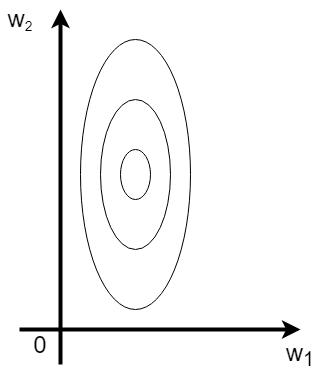
\includegraphics[width=6cm]{8_appendix/img/preprocess_lossfunc}
            \caption{A simplified diagram of how the solution space of the loss function is distorted by the scale of the parameters.}
            \label{locc_func_scale}
        \end{center}
    \end{figure}

    この損失関数で勾配を計算すると,毎回パラメータが大きく更新され,パラメータは更新のたびに大きく振動することとなり,最適化が困難になる.
    通常,機械学習で用いられるデータは$0.3<|x|<3$程度に調整されることが多い.
    このようなスケールに収めるために,以下に示すようなMin-Max Normalization(式\ref{min_max_norm})やZ-score Normalization(式\ref{z_norm})を用いてデータを正規化することが多い.
    \begin{equation}
        x_{new} = (x - x_{min}) / (x_{max} - x_{min})
        \label{min_max_norm}
    \end{equation}
    \begin{equation}
        x_{new} = (x - x_{\rm{mean}}) / x_{\rm{std}}
        \label{z_norm}
    \end{equation}

\subsection{誤差逆伝播法}
    前項において非常に複雑なニューラルネットワークを勾配によって最適化することを示した.
    線形回帰やロジスティック回帰はパラメータはたかだか一度の非線形変換を施されているだけであり,非線形変換が微分可能であれば各パラメータについて勾配を求めるのは容易である.
    しかし,ニューラルネットワークの場合には多数の非線形変換が繰り返し適用されており,個々のパラメータの勾配計算が困難である.
    この学習の困難さが長らくパーセプトロンによるニューラルネットワークの発展の障害となっていた.
    しかしその後,1986年に\cite{rumelhart1986learning}らによって誤差逆伝搬法が提案され,その問題が解決された.

    誤差逆伝搬法とは,入力$x$に対して,目標とする出力$t$と実際の$x$をニューラルネットワークに入力し,得られた出力${y}$の誤差から,ニューラルネットワークを構成するニューロンのパラメータを更新し,入力$x$に対してより目標に近い$y$が出力できるよう効率的に学習するアルゴリズムである.以下\ref{fig:neural_net_with_f}のような,入力層,隠れ層,出力層で構成された,順伝播型ニューラルネットワークが誤差逆伝搬法によってどのように学習されるか説明する.
    \begin{figure}[ht]
        \centering
        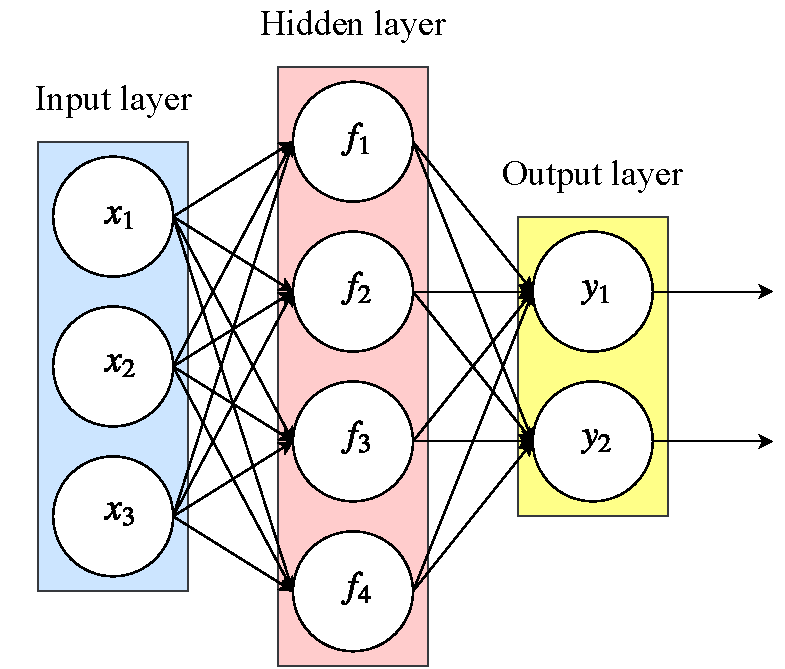
\includegraphics[width=12cm]{8_appendix/img/three_layer_nn.pdf}
        \caption{Three-layer feed-forward neural network.}
        \label{fig:neural_net_with_f}
    \end{figure}
    一方で,最終的な出力は各層の各ニューロンのネットワークの重みやバイアスによって定まるため,ニューラルネットワークの重みやバイアスといったそれぞれのパラメータをどのように更新すれば良いのか求める必要がある.
    ここで,誤差$E$はネットワーク上のすべてのパラメータに関する関数として考えられるため,ネットワークの重みやバイアスと言った学習パラメータ$p$に対して上記のニューラルネットワークの出力$\bm{y}$の更新条件と同様な条件が成り立ち,式\ref{eq:e_y_result}と同様に更新することが出来れば良い.したがって以下の式が成り立つ.
    \begin{align}
      p \to p - \eta \frac{\partial E}{\partial p}
      \label{eq:p_y_result}
    \end{align}
    このように,学習パラメータをある評価関数の勾配に基づいて更新を繰り返し,学習を行うアルゴリズムを最急降下法という.誤差逆伝搬法においては,このアルゴリズムを用いて学習行う.
    
    次に,誤差逆伝搬法において効率的に各パラメータに関する勾配を求める方法について説明する.
    全$\text{N}$層の順伝播型ニューラルネットワークについて,$n$番目の層の$m$番目のニューロンの入出力を考える.\ref{fig:n_layer_network}にネットワーク全体の概要図と,\ref{fig:n_layer_eq}に$m$番目のニューロンの入出力に注目した図を示した.ただし,$n-1$番目の層の$i$番目のニューロンと$n$番目の層の$m$番目のニューロン間の重みを$w_{n, i, m}$,$n$番目の層の$m$番目のニューロンのバイアスを$b_{n, m}$, 入力を$I_{n, m}$, 出力を$x_{n, m}$,活性化関数を$\phi _{n, m}$とした.また$n$番目の層のニューロンの総数を$N_{n}$とした.
    \begin{figure}[ht]
      \centering
      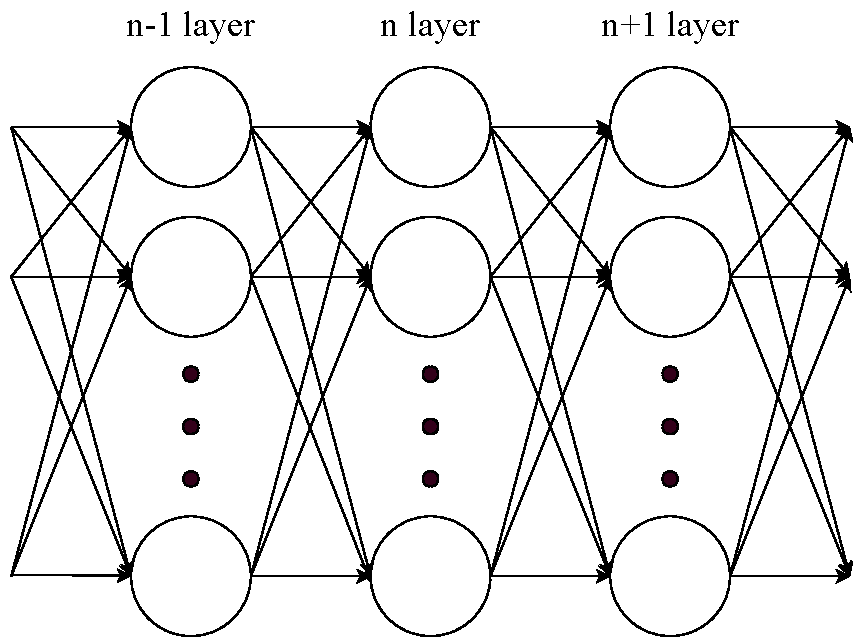
\includegraphics[width=12cm]{8_appendix/img/n_layer_network.pdf}
      \caption{N-layers neural network.}
      \label{fig:n_layer_network}
    \end{figure}
    \begin{figure}[ht]
      \centering
      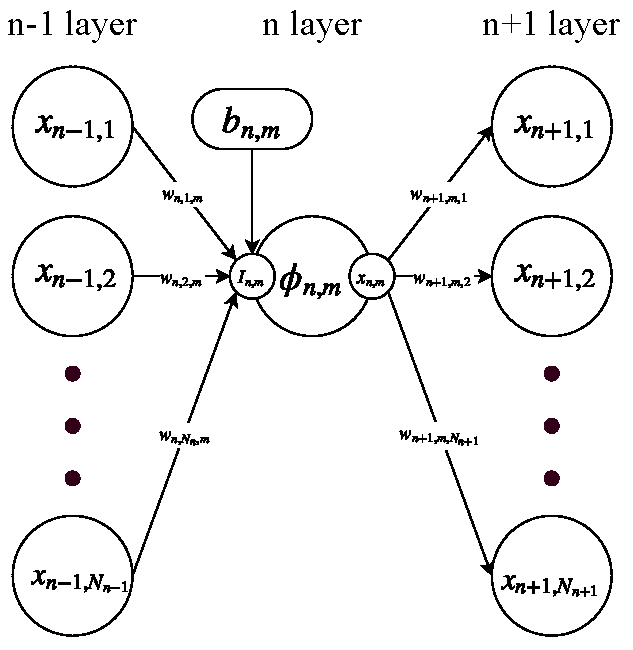
\includegraphics[width=12cm]{8_appendix/img/n_layer_eq.pdf}
      \caption{Neuron $m$ in n-layers neural network.}
      \label{fig:n_layer_eq}
    \end{figure}
    このとき,入出力関係は次式のように表される.
    \begin{align}
      I_{n, m} &= \sum_{k}^{N_{n}} w_{n, k, m} \cdot x_{n-1, k} + b_{n, m} \label{eq:i_nm} \\
      x_{n, m} &= \phi_{n, m}(I_{n, m}) \label{eq:x_nm}
    \end{align}
    次に,$n+1$層を出力層$N$としたときの,$n$層の$i$番目のニューロンと$n+1$層の$j$番目のニューロン間の重み$w_{n+1, i, j}$とバイアス$b_{n+1, j}$がどのように更新されるか求める.
    つまり,式\ref{eq:p_y_result}のように,誤差$E$を各パラメータで偏微分した値を求める.
    まず,重み$w_{n+1, i, j}$に関して,連鎖律より次式で表される.
    \begin{align}
      \frac{\partial E}{\partial w_{n+1, i, j}} &= \frac{\partial E}{\partial x_{n+1, j}} \cdot \frac{\partial x_{n+1, j}}{\partial I_{n+1, j}} \cdot \frac{\partial I_{n+1, j}}{\partial w_{n+1, i, j}}
      \label{eq:w_nim}
    \end{align}
    ここで,$\frac{\partial x_{n+1, j}}{\partial I_{n+1, j}}$,$\frac{\partial I_{n+1, j}}{\partial w_{n+1, i, j}}$は式\ref{eq:i_nm},\ref{eq:x_nm}より次式で表される.
    \begin{align}
      \frac{\partial x_{n+1, j}}{\partial I_{n+1, j}} &= \frac{\partial \phi_{n+1, j}(I_{n+1, j})}{\partial I_{n+1, j}} \nonumber \\
          &= \phi_{n+1, j}^{'}(I_{n+1, j}) \cdot (I_{n+1, j})' \nonumber \\
          &= \phi_{n+1, j}^{'}(I_{n+1, j})
          \label{eq:n_1}
    \end{align}
    \begin{align}
      \frac{\partial I_{n+1, j}}{\partial w_{n+1, i, j}} &= \frac{\partial \left( \sum_{k}^{N_{n+1}}w_{n+1, k, j}x_{n, k} + b_{n+1, j}\right)}{\partial w_{n+1, i, j}} \nonumber \\
      &= x_{n, i}
          \label{eq:n_2}
    \end{align}
    よって式\ref{eq:n_1}, \ref{eq:n_2}を式\ref{eq:w_nim}に代入すると
    \begin{align}
      \frac{\partial E}{\partial w_{n+1, i, j}} &= \frac{\partial E}{\partial x_{n+1, j}} \cdot \phi_{n+1, j}^{'}(I_{n+1, j}) \cdot x_{n, i} \label{eq:ew_n1ij}
    \end{align}
    となる.
    またバイアス$b_{n, m}$に関しても同様に計算を行うと,次式で表される.
    \begin{align}
      \frac{\partial E}{\partial b_{n+1, j}} &= \frac{\partial E}{\partial x_{n+1, j}} \cdot \phi_{n+1, j}^{'}(I_{n+1, j})
    \end{align}
    したがって,$\frac{\partial E}{\partial x_{n+1, j}}$が計算できればそれぞれのパラメータを更新することが出来る.
    
    ここで,同様の計算を$n-1$層と$n$層間でも行う.
    つまり,$n-1$層の$s$番目のニューロンと$n$層の$t$番目のニューロン間の重み$w_{n, s, t}$とバイアス$b_{n, t}$がどのように計算されるか求める.
    ここで,\ref{fig:n_layer_eq}のように,$n$層の$t$番目のニューロンが$n+1$層の$N_{n+1}$個のニューロン全てと繋がっており,これらの出力の変化に$w_{n, s, t}$が関係していることに注意し,鎖律より$ \frac{\partial E}{\partial w_{n, s, t}} $を求めると,次式のようになる.
    \begin{align}
      \frac{\partial E}{\partial w_{n, s, t}} &= \sum_{k}^{N_{n+1}}\left( \frac{\partial E}{\partial x_{n+1, k}}\cdot 
      \frac{\partial x_{n+1, k}}{\partial I_{n+1, k}}\cdot \frac{\partial I_{n+1, k}}{\partial x_{n, t}} \right)
      \cdot \frac{\partial x_{n, t}}{\partial I_{n, t}} \cdot \frac{\partial I_{n, t}}{\partial w_{n, s, t}}
      \label{eq:w_nst}
    \end{align}
    このとき,式\ref{eq:n_1}より
    \begin{align}
      \frac{\partial x_{n+1, k}}{\partial I_{n+1, k}} &= \phi _{n+1, k}(I_{n+1, k})
      \label{eq:x_n1k}
    \end{align}
    また$\frac{\partial I_{n+1, k}}{\partial x_{n, t}} $は以下の式で表される.
    \begin{align}
      \frac{\partial I_{n+1, k}}{\partial x_{n, t}} &= \frac{\sum_{i}^{N_{n+1}}w_{n+1, i, j}x_{n, i} + b_{n+1, j}}{\partial x_{n, t}} \nonumber \\
      &= w_{n+1, t, k}
      \label{eq:i_n1k}
    \end{align}
    よって,\ref{eq:w_nst}は式\ref{eq:x_n1k},\ref{eq:i_n1k}より次のようになる.
    \begin{align}
      \frac{\partial E}{\partial w_{n, s, t}} &= \sum_{k}^{N_{n+1}} \left( \frac{\partial E}{\partial x_{n+1, k}} \cdot \phi_{n+1, l}'(I_{n+1, k})\cdot w_{n+1, t, k} \right) \phi_{n, t}'(I_{n, t}) \cdot x_{n-1, s} 
    \end{align}
    ここで,$\frac{\partial E}{\partial x_{i, j}}\cdot \phi_{i, j}'(I_{i,j})$は既に$n$層と$n+1$層間でのニューロンの重みに関する式\ref{eq:ew_n1ij}にて既に計算されているため,これを$\delta_{i, j}$として整理すると次のようになる.
    \begin{align}
      \frac{\partial E}{\partial w_{n, s, t}} &= \sum_{k}^{N_{n+1}} \left( \delta_{n+1, k}\cdot w_{n+1, t, k} \right) \phi_{n, t}'(I_{n, t}) \cdot x_{n-1, s} \label{eq:ew_nst}
    \end{align}
    バイアスについても同様に次のようになる.
    \begin{align}
      \frac{\partial E}{\partial b_{n, t}} &= \sum_{k}^{N_{n+1}} \left( \delta_{n+1, k}\cdot w_{n+1, t, k} \right) \phi_{n, t}'(I_{n, t}) 
      \label{eq:eb_nt}
    \end{align}
    これらの式より,各層間での重みやバイアスといったニューラルネットワークの各パラメータを更新することで,学習することができる.
    
    また順伝播後に出力層から入力層へと順々に上記の計算を繰り返し行うことで,前層で既に求められている勾配を活用しながら各層間の各ニューロン間の重みとバイアスを更新するための勾配を求めることが出来る.
    このように,勾配を計算するための誤差が層を逆方向に伝播されて計算が行われるため,この手法は誤差逆伝搬法と呼ばれる.

    この誤差逆伝搬法によってニューラルネットワークを学習させるためには,活性化関数が微分可能である必要がある.
    そこで,パーセプトロンにおけるステップ関数を置き換えるためにシグモイド関数が活性化関数として提案された\cite{rumelhart1986learning}.
    しかし,ReLuを始めとする微分不可能な点が存在する関数は多く活性化関数として使われており,実用上は微分不可能な点が存在していても問題がないことも広く知られている.
    ただし,ステップ関数は微分値が常に0であり,誤差の逆伝播計算値が常に0となるため,誤差逆伝播を用いて最適化を行うモデルでこのような活性化関数を利用することはできない.

    また,sigmoid関数の微分値を見てみると,sigmoid関数の微分値は以下の図\ref{sigmoid_diff}のように最大値が0.25である.
    \begin{figure}[ht]
        \begin{center}
            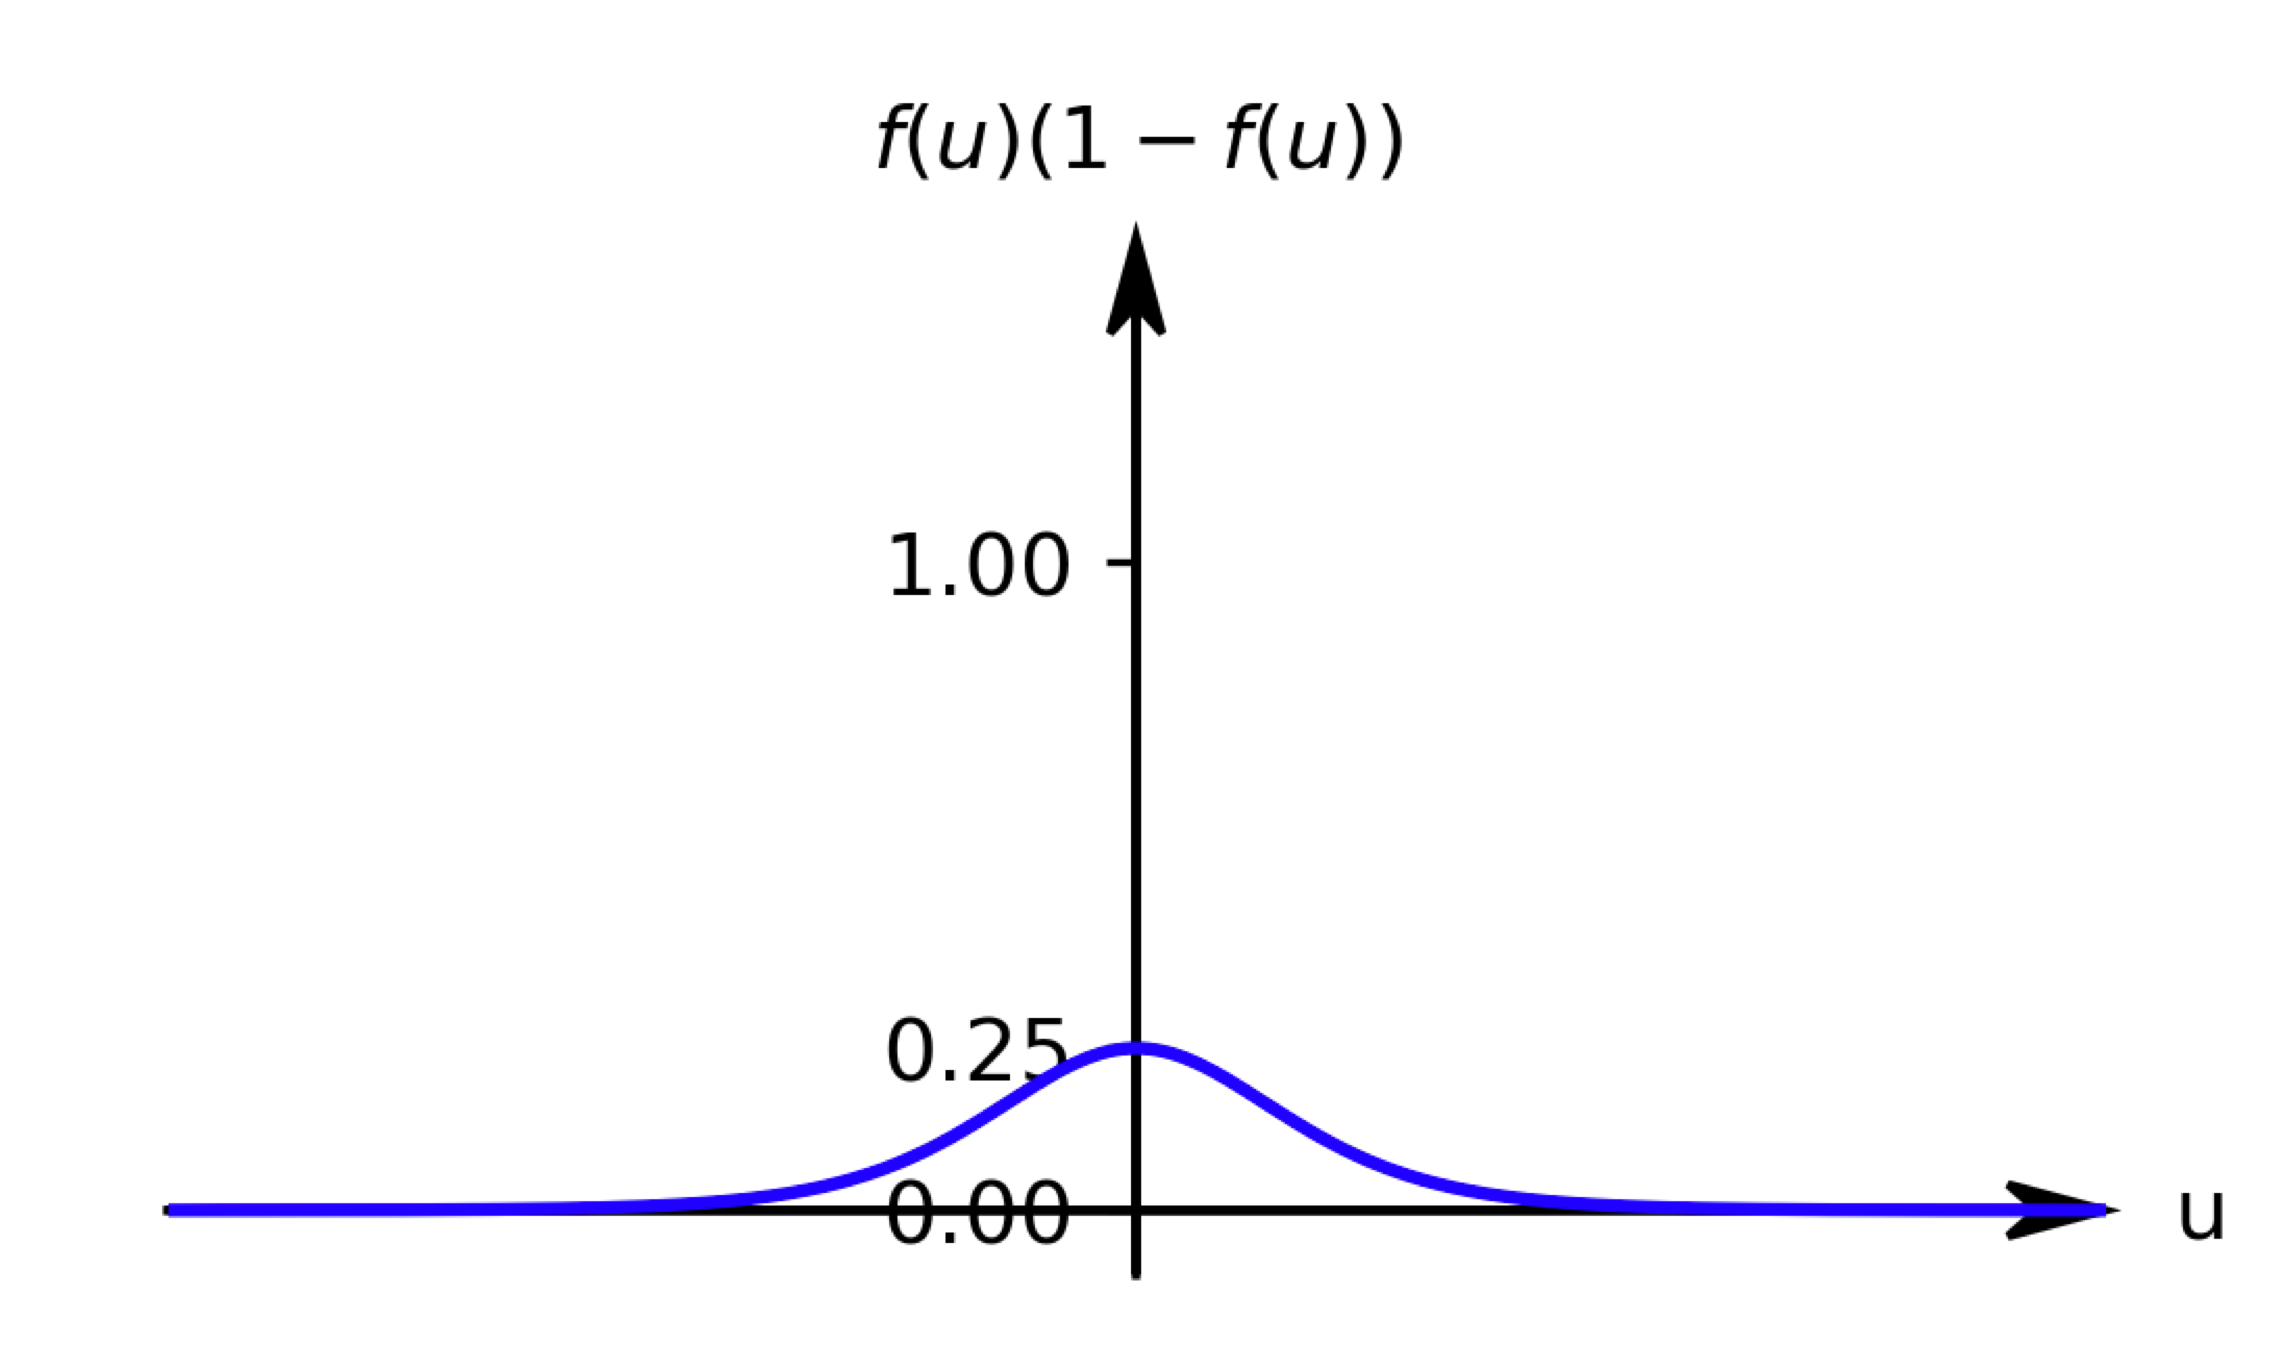
\includegraphics[width=10cm]{./8_appendix/img/sigmoid_diff.png}
            \caption{Derivatives of sigmoid functions.}
            \label{sigmoid_diff}
        \end{center}
    \end{figure}
    これは逆伝播計算の際に,繰り返しシグモイド関数が適用されるニューラルネットの浅い層になるほど,勾配の値が小さくなってしまうことを示している.
    このように浅い層になるほど勾配の値が小さくなり,深いネットワークでは浅い層に対する勾配が0付近になってしまうような現象のことを勾配消失と呼ぶ.
    これを避けるために,ニューラルネットの中間層ではReLU関数など,微分値が1に近いかそれ以上になるような活性化関数が用いられることが多い.

\subsection{様々な最適化手法}
    前項では,勾配による最適化をどのように行うかについて議論してきた.
    本項では確率的勾配降下法を改善し,勾配法の学習を最適化させる様々な手法について触れる.
    
    \subsubsection{モメンタム}
    SGDの学習をより効率的に行う方法は,大別して1次の方法および2次の方法に分類される.
    一般的にニューラルネットワークの学習では1次の方法が用いられている.
    モメンタム\cite{polyak1964some}(Momentum)は1次の方法の中でも最も一般的に使われる手法の1つで,一期前の更新量を保存することにより,更新されるパラメータの慣性を持ったような動きを実現する.
    SGDは一定の学習率を持つために学習が遅くなる傾向があるのに対し,モメンタムは学習を高速化するために設計されている.
    Momentumにおけるパラメータの更新式は以下の通りである.
    \begin{eqnarray}
        v_{t+1} &=& \alpha v_t - \eta \frac{\partial L}{\partial \theta_t}\\
        \theta_{t+1} &=& \theta_t + v_{t+1}
    \end{eqnarray}
    ここで,$\eta$は学習率を,$\alpha$はモメンタム係数を示す.($0\leq\alpha<1$)
    
    \subsubsection{Nesterov Accelerated Gradient}
    Nesterov AG\cite{mikolov2013distributed}はネステロフの加速勾配法\cite{nesterov1983method}に着想を得て開発されたモメンタムの派生系である.
    このアルゴリズムでは,一期先の位置を仮に決定し,その位置における勾配を利用することにより更新値を算出する.
    Nesterov AGにおけるパラメータの更新式を以下に示す.
    \begin{eqnarray}
        v_{t+1} &=& \alpha v_t - \eta \frac{\partial L}{\partial (\theta_t+\alpha v_t)}\\
        \theta_{t+1} &=& \theta_t + v_{t+1}
    \end{eqnarray}
    Nesterov AGを定義通りに計算するのは一期先の勾配が必要となり,計算が煩雑になる.
    したがって,現在ではBengioら\cite{bengio2013advances}が提案したアルゴリズムを採用して計算されることが多い.
    
    Nesterov AGがSGDおよびモメンタムとどのような差があるかを図\ref{SGD_update}から図\ref{Nesterov_update}で示した.
    \begin{figure}[ht]
        \begin{center}
            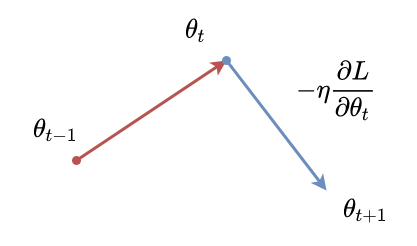
\includegraphics[width=6cm]{./8_appendix/img/SGD.png}
            \caption{Schematic diagram of parameter updates with SGD.}
            \label{SGD_update}
        \end{center}
    \end{figure}
    \begin{figure}[ht]
        \begin{center}
            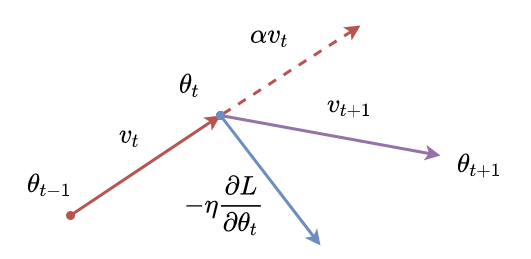
\includegraphics[width=8.5cm]{./8_appendix/img/momentum.png}
            \caption{Schematic diagram of parameter updates with Momentum.}
        \end{center}
    \end{figure}
    \begin{figure}[ht]
        \begin{center}
            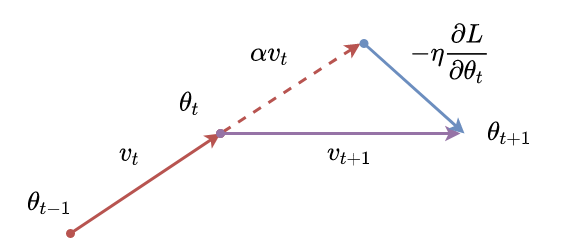
\includegraphics[width=8.5cm]{./8_appendix/img/Nesterov.png}
            \caption{Schematic diagram of parameter updates with Nesterov AG.}
            \label{Nesterov_update}
        \end{center}
    \end{figure}

    \subsubsection{AdaGrad}
    先述までの手法では学習率は任意に設定できるハイパーパラメータである上に,モデルの性能に大きな影響を与えるものであった.
    故に,学習率を損失の計算時に適応的(adaptive)に変化させる手法が多く提案されている.
    Adagrad\cite{duchi2011adaptive}はそのような適応的に学習率が変化するような手法の1つであり,学習が進むにつれ見かけの学習率が減衰していくように設計されている.
    この手法において,学習率は過去の学習率の二乗和の平方根に反比例するようにスケーリングされる.
    Adagradにおけるパラメータの更新式を以下に示す.
    \begin{eqnarray}
        \boldsymbol{h}_{t+1} &=& \boldsymbol{h}_{t}+\frac{\partial L}{\partial \boldsymbol{\theta}_{t}} \odot \frac{\partial L}{\partial \boldsymbol{\theta}_{t}} \\
        \boldsymbol{\theta}_{t+1} &=& \boldsymbol{\theta}_{t}-\eta \frac{1}{\varepsilon+\sqrt{\boldsymbol{h}_{t+1}}} \odot \frac{\partial L}{\partial \boldsymbol{\theta}_{t}}
    \end{eqnarray}
    ここで,$\varepsilon$は数値的安定性のために導入されている微小値であり,通常およそ$10^{-7}$に設定されている.
    また,$\odot$はアダマール積を表す.

    学習が進むにつれて見かけの学習率である$1/\varepsilon+\sqrt{\boldsymbol{h}_{t+1}}$が減衰することが分かる.
    しかし,AdaGradは学習は学習初期から勾配の2乗の累計を計算するために,学習率が過剰に減衰する.
    そのため,経験的にはAdaGradは常に良好な結果を残す最適化手法ではないことが知られている.
    
    \subsubsection{RMSProp}
    RMSProp\cite{hinton2012neural}は先述のAdaGradを修正し,勾配の二乗の移動平均を用いて見かけの学習率を変化させることによって,AdaGradの性能を改善させた.
    ここで,移動平均とは指数平滑化移動平均のことであり,減衰率$\rho$の割合で過去の勾配を足し合わせることにより,累積される情報は過去のものから指数関数的に減衰していく.
    RMSPropにおけるパラメータの更新式を以下に示す.
    \begin{eqnarray}
        \boldsymbol{h}_{t+1} &=& \rho \boldsymbol{h}_{t}+(1-\rho) \frac{\partial L}{\partial \boldsymbol{\theta}_{t}} \odot \frac{\partial L}{\partial \boldsymbol{\theta}_{t}} \\
        \boldsymbol{\theta}_{t+1} &=& \boldsymbol{\theta}_{t}-\eta \frac{1}{\sqrt{\varepsilon+\boldsymbol{h}_{t+1}}} \odot \frac{\partial L}{\partial \boldsymbol{\theta}_{t}}
    \end{eqnarray}
    
    \subsubsection{AdaDelta}
    AdaDelta\cite{zeiler2012adadelta}も先述のRMSPropと同様にAdaGradを修正した最適化手法の1つである.
    RMSPropが勾配の二乗の移動平均のみを用いて学習率を変化させるのに対し,AdaDeltaは勾配の二乗の移動平均に加えて,更新量の二乗の移動平均を用いて見かけの学習率を変化させる.
    AdaDeltaにおけるパラメータの更新式を以下に示す.
    \begin{eqnarray}
        \boldsymbol{h}_{t+1}&=&\rho \boldsymbol{h}_{t}+(1-\rho) \frac{\partial L}{\partial \boldsymbol{\theta}_{t}} \odot \frac{\partial L}{\partial \boldsymbol{\theta}_{t}} \\
        \Delta \boldsymbol{\theta}_{t}&=&-\frac{\sqrt{\varepsilon+\boldsymbol{r}_{t}}}{\sqrt{\varepsilon+\boldsymbol{h}_{t+1}}} \odot \frac{\partial L}{\partial \boldsymbol{\theta}_{t}} \\
        \boldsymbol{\theta}_{t+1}&=&\boldsymbol{\theta}_{t}+\Delta \boldsymbol{\theta}_{t} \\
        \boldsymbol{r}_{t+1}&=&\rho \boldsymbol{r}_{t}+(1-\rho) \Delta \boldsymbol{\theta}_{t} \odot \Delta \boldsymbol{\theta}_{t}
    \end{eqnarray}
    上記のように,更新量の二乗の移動平均を導入することにより,極小値付近でこの値が非常に小さい値になり,動きが遅くなる.
    また,学習率$\eta$が更新量の移動平均と置き換えられ,単位を揃える働きをしていることに注意されたい.
    
    \subsubsection{Adam}
    Adam\cite{kingma2014adam}はRMSpropおよびモメンタムを同時に適用したような手法であり,学習率の変化にも頑健で,現在最も良く利用されている最適化手法の1つに数えられる.
    AdamとRMSpropおよびモメンタムには若干の差が存在する.
    Goodfellowら\cite{Goodfellow-et-al-2016}は以下の2つの差異を指摘している.
    1つ目は,モメンタムをRMSpropに追加する最も単純な方法は,再スケーリングされた勾配にモメンタムを適用することだが,Adamでは式\ref{adam_momentum}のように,1次モーメントが直接導入されていることである.
    そして,2つ目は1次モーメントおよび2次モーメント両方の推定へのバイアス補正が含まれており,原点での初期化が考慮されていない点である.
    
    \begin{eqnarray}
        \boldsymbol{m}_{t+1} &=&\rho_{1} \boldsymbol{m}_{t}+\left(1-\rho_{1}\right) \frac{\partial L}{\partial \boldsymbol{\theta}_{t}} \label{adam_momentum}\\
        \boldsymbol{v}_{t+1} &=&\rho_{2} \boldsymbol{v}_{t}+\left(1-\rho_{2}\right) \frac{\partial L}{\partial \boldsymbol{\theta}_{t}} \odot \frac{\partial L}{\partial \boldsymbol{\theta}_{t}} \\
        \widehat{\boldsymbol{m}}_{t+1} &=&\frac{\boldsymbol{m}_{t+1}}{1-\rho_{1}^{t}} \\
        \widehat{\boldsymbol{v}}_{t+1} &=&\frac{\boldsymbol{v}_{t+1}}{1-\rho_{2}^{t}} \\
        \boldsymbol{\theta}_{t+1} &=&\boldsymbol{\theta}_{t}-\eta \frac{1}{\sqrt{\hat{\boldsymbol{v}}_{t+1}}+\varepsilon} \odot \widehat{\boldsymbol{m}}_{t+1}
    \end{eqnarray}

\subsection{深層学習における正則化}
    過学習はニューラルネットワークの学習においても発生する.
    過学習は訓練誤差に比べ汎化誤差が大きくなる現象であり,パラメータが多い場合や,訓練データの数が少ない場合などに発生しやすい.
    その意味で言えばニューラルネットワークは膨大なパラメータを有しているために,過学習が非常に起きやすい.
    この過学習に対応するために,パラメータに制限を設けるなどの対応が行われ,これは正則化と呼ばれている.
    本節では,前節で触れたL2正則化に触れつつ,ニューラルネットワークの訓練における正則化手法を複数示す.

    \subsubsection{荷重減衰}
    荷重減衰(weight decay)は最も一般的な正則化手法の1つであり,重みの値が大きくなることにペナルティを与えることによって過学習を抑制している.
    荷重減衰では,損失関数の全ての層に$1/2\lambda w_{ij}^2$を加える.
    これは前節で触れたL2正則化と同様であり,この項をL2ノルムと呼ぶ.
    ここで$\lambda$は通常$1.0^{-2}$~$1.0^{-5}$程度の値が利用されることが多い.
    また,ニューラルネットワークにおける荷重減衰は,アフィン変換の重みにのみ適用され,通常バイアス項には適用されないことに注意されたい.

    \subsubsection{早期終了}
    早期終了(early stoppting)は,一定のルールを満たした場合に学習を終了させる手法であり,一般に過学習抑制効果がある\cite{bishop1995regularization,sjoberg1995overtraining}.
    早期終了の学習終了基準は非常に単純である.
    学習の各ステップにおけるテスト用データの検証誤差(validation loss)を算出し,前ステップの検証誤差と比較する.
    現ステップの検証誤差が前ステップよりも高かった場合カウンタに1を加算し,このカウンタが指定回数以上になった場合に学習を終了させる.
    ここでの指定回数はハイパーパラメータとなる.
    
    \subsubsection{ドロップアウト}
    ドロップアウト\cite{srivastava2014dropout}(dropout)は,ノードをランダムに消去しながら学習する方法であり,過学習を抑制する効果がある.
    過学習抑制に有効な手法としてアンサンブル学習があり,アンサンブル学習の中でも複数のモデルを組み合わせて予測を頑健にする手法をバギングと呼ぶ.
    バギングは非常に計算コストが高く実用的でない場合が多い.
    ドロップアウトは,複数のネットワークをアンサンブル学習していると解釈できることから,バギングの近似であると表現されることがある.
    
    ドロップアウトの発想は比較的簡単である.
    各ミニバッチに対して,消去するノードを確率$p$でランダムに選択し,順伝播計算および逆伝播計算を行う.
    このとき,消去したノードは順伝播および逆伝播のどちらでも使うことはない.
    そして,予測時には全てのノードを採用する.このとき,全ての重みに$(1-p)$を一律で掛け合わせる.
    この操作は全てのノードを採用することによって,学習時に比べて出力値が大きくなることを是正している.
    \begin{figure}[ht]
        \begin{center}
            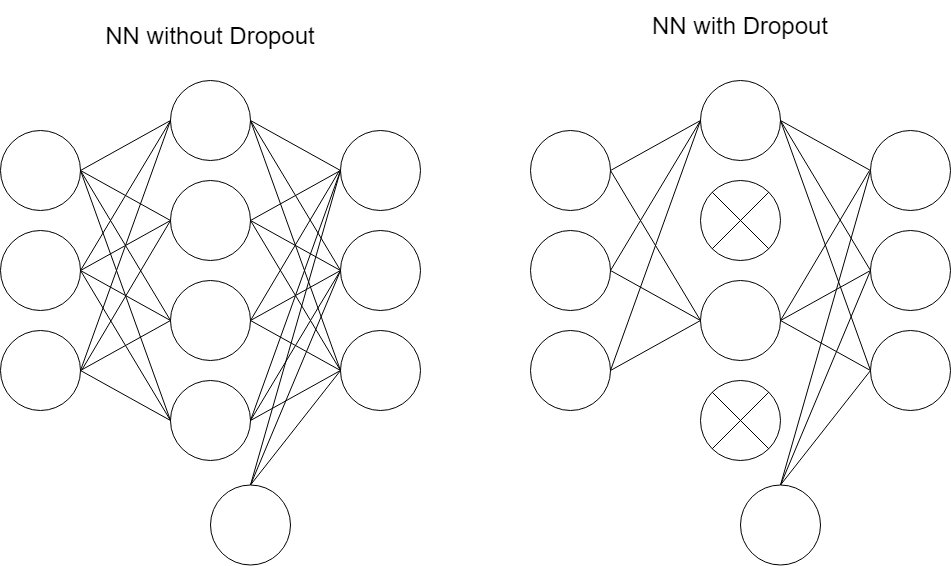
\includegraphics[width=12cm]{./8_appendix/img/dropout.png}
            \caption{Dropout}
        \end{center}
    \end{figure}

    ドロップアウトは特に全結合層に対してのみ適用されることが多く,畳込み層に適用される機会は少ない.
  原著論文\cite{srivastava2014dropout}では畳み込み層が持つパラメータが少ないため、ドロップアウトが持つ正則化の効果が薄くなることを指摘している。
    
    \subsubsection{バッチ正規化}
    バッチ正規化\cite{ioffe2015batch}(batch normalization)とは各層のアクティベーション分布を適度な広がりを持つように調整する手法であり,活性化関数の手前に設置されることが多い.
    バッチ正規化により,学習の進行が速くなることが期待でき,ネットワークの初期値に依らない学習が可能になる.
    バッチ正規化は本来,内部共変量シフトの解決を目的に設計されたが,結果的に正則化の効果を得られることが多い.
    内部共変量シフトとは,ニューラルネットワークにおいて発生する共変量シフトのことである.
    共変量とはモデルに入力されるデータのことであり,この入力に対する出力の生成規則は訓練時とテスト時で変わらないが,入力 (共変量) の分布が訓練時とテスト時で異なるという状況のことを変量シフトと呼ぶ.
    例えば,ニューラルネットワークではステップごとにパラメータが更新され,n層目の出力(n+1層目の入力)の分布は重みが更新されるたびに変化する.
    バッチ正規化を用いることで,この共変量シフトへの対応を,一層前のパラメータ全体から,バッチ正規化の持つパラメータのみに絞ることができ,効率的な学習が可能となる.
    
    バッチ正規化の計算手順は,仮に計算対象を式\ref{cal_x}のように定めると式\ref{standlization}のように計算できる.
    \begin{equation}
        \bm{x} = \{x_1,x_2, ... ,x_n\}
        \label{cal_x}
    \end{equation}
    \begin{equation}
        y_i = \gamma \frac{x_i-\mu}{\sqrt{\sigma^2+\epsilon}} + \beta
        \label{standlization}
    \end{equation}
    
    ここで,$\beta,\gamma$は標準化された$x$の分布を最適な分布に変換するための係数であり,学習の過程で最適化されていくパラメータである.
    ここで,データの平均値および分散を表す$\mu,\sigma^2$について,予測時には学習時の移動平均を用いることに注意されたい.
    
    バッチ正規化は、現在ほとんどのモデルで導入されている。
    また、特にバッチ正規化はドロップアウトと併用されることはない。
    特に、バッチ正規化の直後にドロップアウトを使用することにより、バッチ正規化によって得られた統計的性質が阻害されるために、精度の悪化などの悪影響が報告されている\cite{li2019understanding} 。
    
    また、バッチ正規化は基本的に荷重減衰と併用することはあまり意味がないとされている。
    これは、バッチ正規化が出力スケールを入力によらず不変にするためである。
    バッチ正規化に入力される値のスケールはレイヤの重みのスケールと線形関係にある。
    バッチ正規化の出力スケールが入力によらず不変になるのであれば、モデルの重みを制限することによりレイヤーの異常な出力を抑制している荷重減衰を適用するかどうかに関わらず、バッチ正規化の出力スケールは不変であり、荷重減衰を適用する利点は薄い。
    しかし、荷重減衰を適用することにより学習率が過剰に低下するのを防止する効果も見られることから、この観点で荷重減衰を利用することは考えられる。
    この議論は様々な論文で指摘されている\cite{van2017l2, hoffer2018norm}。

    また,バッチ正規化の他にも,類似の手法がいくつか提案されている.
    例えば,レイヤー正規化\cite{ba2016layer}では,バッチ方向ではなく,レイヤーの内部のみで各データについて正規化を行っている.
    また,インスタンス正規化\cite{ulyanov2016instance}では,さらに画像内のチャンネルにのみ注目した正規化を行っている.
    これは,1チャンネル分の画像で正規化することにより,画像のコントラストを取り除くことを意図している.
    そして,グループ正規化\cite{wu2018group}では,インスタンス正規化のようにチャンネルに注目し,そのチャンネルを複数のグループにまとめてから正規化を行っている.
    これは,バッチサイズを小さくするとバッチごとの統計量の推定精度が劣化することに注目して,バッチサイズの影響を受けないような設計になっている.
    \begin{figure}[ht]
        \begin{center}
            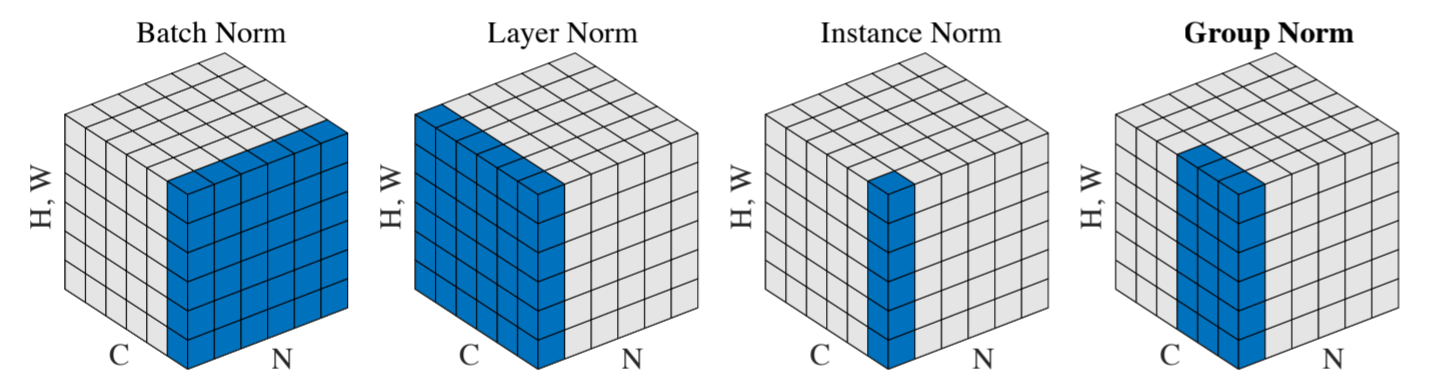
\includegraphics[width=15cm]{./8_appendix/img/batchnorm_description}
            \caption{A brief description of each normalization method\cite{wu2018group}.}
        \end{center}
    \end{figure}


\section{畳み込みニューラルネットワーク}
2012年,Alexnet\cite{krizhevsky2012imagenet}によって畳み込みニューラルネットワークを用いた画像認識手法がこれまでの既存の手法を遥かに上回る性能を提示して以来,コンピュータビジョンの分野において畳み込みニューラルネットワーク(Convolutional Neural Netowrk : CNN)を用いたアルゴリズムは必要不可欠な手法となった.
畳み込みニューラルネットワークとは,コンピュータビジョンの分野において,現在最も成果を挙げているニューラルネットワークの構造の一つである.
畳み込みニューラルネットワークは畳み込み層とプーリングと呼ばれる演算を中心に構成されるネットワークである.
本節では,畳込みニューラルネットワークの基礎から,著名なモデルの解説まで行う.

\subsection{畳み込み演算}
    本項では,畳み込みニューラルネットワークにおける畳み込み演算について説明する.
    畳み込みニューラルネットワークにおける畳み込み演算は,以前からコンピュータビジョンの分野において画像から特徴量を抽出するために使われている手法をベースとしている.
    畳み込み演算は,画像処理におけるフィルター演算に相当する.
    このフィルターという言葉は,カーネルと表現されることもある.
    畳み込みニューラルネットワークはある特定のテクスチャパターンに反応するように学習されたフィルタを,入力データに対して畳み込み演算をすることで特徴の抽出を行う.
    \begin{figure}[ht]
      \centering
      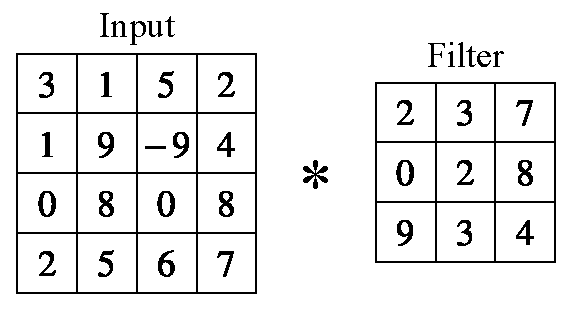
\includegraphics[width=10cm]{8_appendix/img/conv.pdf}
      \caption{Ex) input and filter for convolution.}
      \label{fig:ex_conv_input_filter}
    \end{figure}
    
    ここで例として,入力データが$4 \times 4$の2階のテンソルであり,フィルタのサイズが$3 \times 3$の2階のテンソルである場合を考える.
    このときの畳み込み演算の概要図を\ref{fig:ex_conv_input_filter}に示した.
    また畳み込み演算の計算の過程の模式図を\ref{fig:ex_conv_step_1}から\ref{fig:ex_conv_step_4}に示した.
    入力データからフィルタと同サイズのテンソルを抽出し,それらとフィルタの要素ごとの積(アダマール積$\odot$)を計算した後,その和を計算結果とする.
    これを位置を$N$ピクセルずつずらしながら繰り返し,その位置ごとの結果をまとめたテンソルが出力となる.
    ここで,ずらす量のことストライドと呼ぶ.
    
    \begin{figure}[ht]
      \centering
      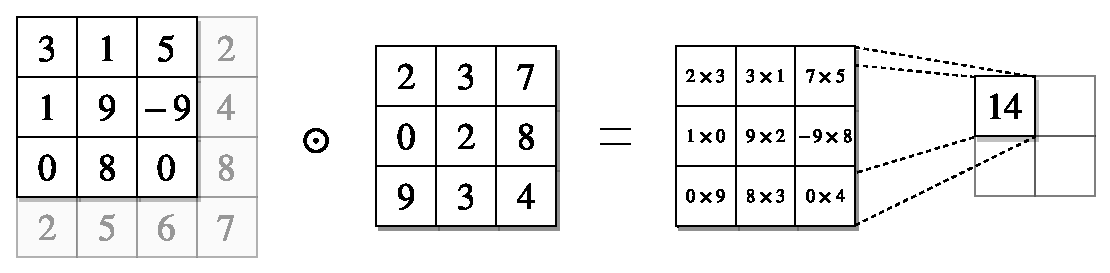
\includegraphics[width=14cm]{8_appendix/img/conv_step_1.pdf}
      \caption{Outline of convolution (Step-1).}
      \label{fig:ex_conv_step_1}
    \end{figure}
    \begin{figure}[ht]
      \centering
      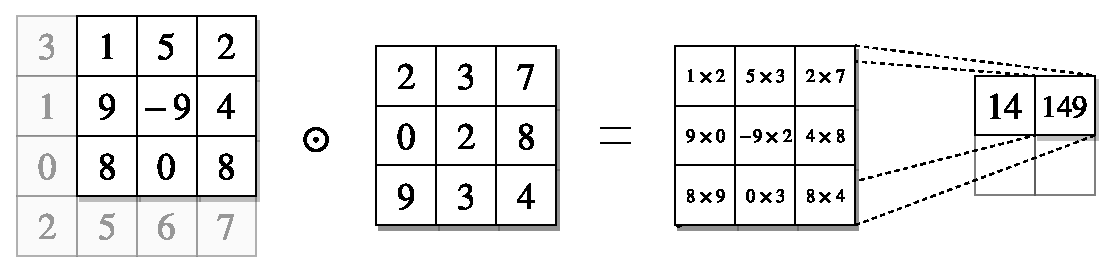
\includegraphics[width=14cm]{8_appendix/img/conv_step_2.pdf}
      \caption{Outline of convolution (Step-2).}
      \label{fig:ex_conv_step_2}
    \end{figure}
    \begin{figure}[ht]
      \centering
      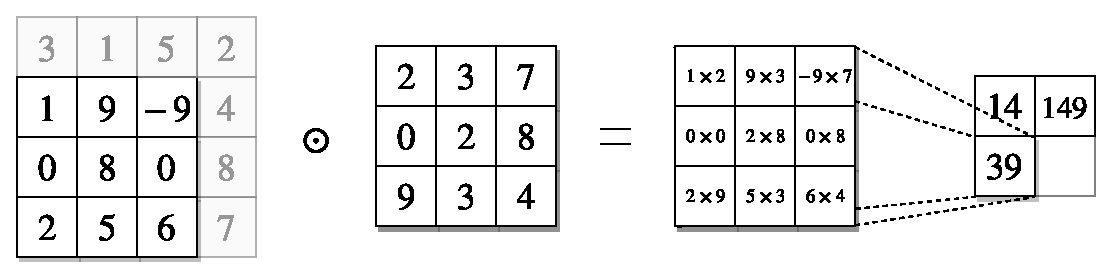
\includegraphics[width=14cm]{8_appendix/img/conv_step_3.pdf}
      \caption{Outline of convolution (Step-3).}
      \label{fig:ex_conv_step_3}
    \end{figure}
    \begin{figure}[ht]
      \centering
      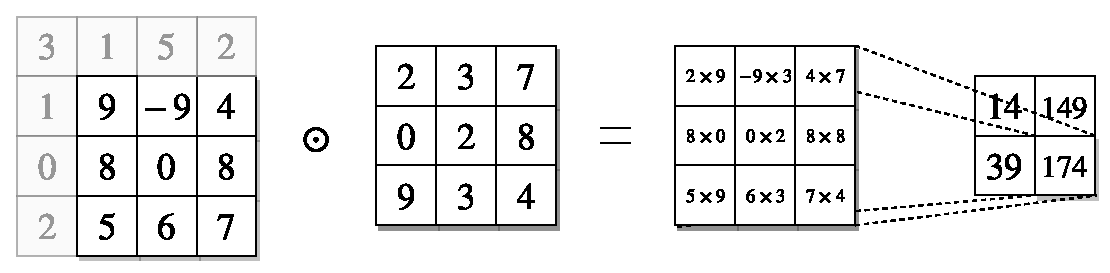
\includegraphics[width=14cm]{8_appendix/img/conv_step_4.pdf}
      \caption{Outline of convolution (Step-4).}
      \label{fig:ex_conv_step_4}
    \end{figure}
    ニューラルネットワークの学習においては,この畳み込みを行うフィルタの各要素のパラメータが学習される.
    一方で,フィルタの形状,大きさやフィルタの位置をずらす量等のパラメータは学習したいデータや抽出したい特徴から設計する必要がある.
    また一般的な畳み込みニューラルネットワークでは,図\ref{fig:outline_of_convolution_3d}のように入力データに対して複数のフィルタを用いて畳み込み演算を行うため,その出力結果は3階のテンソルとなる.
    さらに,畳込み演算の結果に対して更に畳み込み演算が適用されることが多い.例えば,2次元画像を入力データとした場合,そのデータ形状はチャンネル $\times$ 高さ $\times$ 幅となる.
    \begin{figure}[ht]
      \centering
      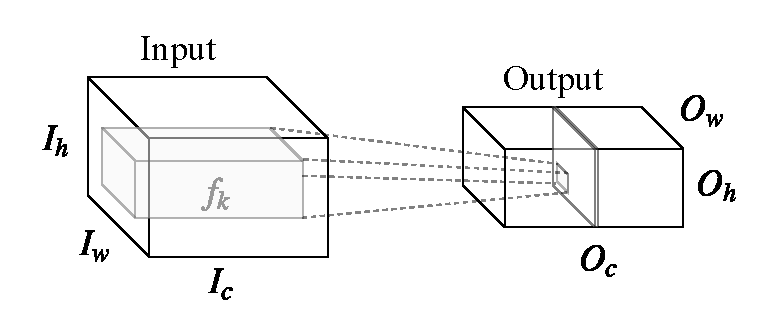
\includegraphics[width=14cm]{8_appendix/img/outline_of_convolution_3d.pdf}
      \caption{Outline of convolution.(3D)}
      \label{fig:outline_of_convolution_3d}
    \end{figure}

    ここで,1つのフィルタで畳込み演算された結果は各チャンネルで加算されることに注意したい.
    また,畳込み演算において,バイアスはフィルタ内の共通のパラメータとして扱われることが多く,演算結果の全ての値に対して適用されることが多い.
    
    重要な点として,畳み込みニューラルネットワークは,多層パーセプトロンと比べてパラメータ数が非常に少ないことが挙げられる.
    多層パーセプトロンでは一つのユニットが次の層のすべてのユニットに結合される全結合層(fully-connected layer)のみを用いて構成されている.
    それ故に, 深い構造になるほどパラメータ数が膨大になり, 学習が困難になる.
    例えば,256$\times$256サイズの画像を入力し,次の層が100ユニットの全結合層だった場合,必要なパラメータは256$\times$256$\times$100となり,膨大な数のパラメータが必要になる.
    一方,カーネルサイズが3,チャンネル数が100の畳み込み演算を行う場合,必要なパラメータは3$\times$3$\times$100と,非常に少ないパラメータでモデルを構成することができる.
    
    \begin{figure}[ht]
        \begin{center}
            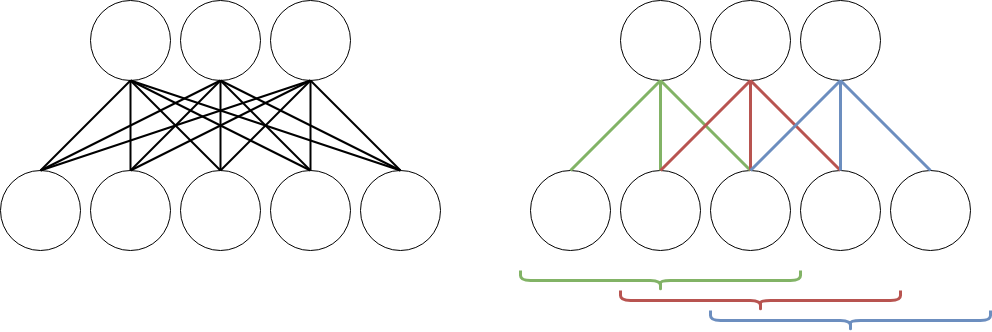
\includegraphics[width=12.0cm]{./8_appendix/img/FCL_conv.png}
            \caption{Comparison of the number of parameters in fully connected layer and convolutional layer.}
            \label{FCL_conv}
        \end{center}
    \end{figure}
    
    また,図\ref{FCL_conv}からも分かる通り, 単純な畳込み操作では画像の最も端にある画素が無くなってしまう.
    この量はカーネルサイズを$k$とすると$k-1$であり,両端で$(k-1)/2$画素の欠損が起こる.
    そのため, 画像サイズを保つためには予め同じだけの画素を付与する必要があり, その操作をパディングと呼ぶ.
    通常は0でパディングを行い,これを特にゼロパディングと呼ぶ.
    ゼロパディングでは, 画像の端の特徴マップが暗くなるなどの欠点もある.

    \begin{figure}[ht]
        \begin{center}
            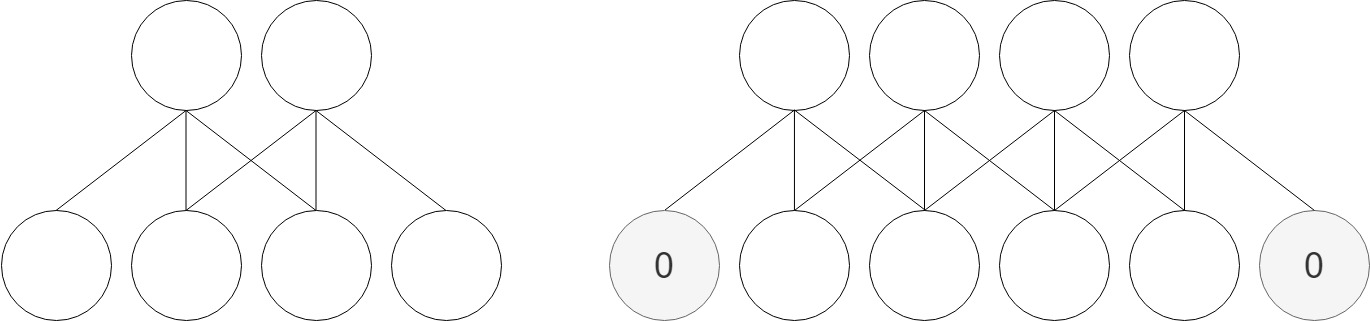
\includegraphics[width=12.0cm]{./8_appendix/img/padding.jpg}
            \caption{Image size can be maintained by zero padding.}
            \label{padding}
        \end{center}
    \end{figure}
    
    また,畳み込み層では実用上カーネルサイズは3が採用されることが多い.
    これは,カーネルサイズが3以上の畳み込み層は,カーネルサイズ3の畳み込みそうを複数重ねることにより表現可能なことに起因する.
    例えば,カーネルサイズが5の畳み込み層はカーネルサイズ3の畳込み層2つを直列に接続した場合と受容野の広さが同一である.

    ここでさらに,畳込み層のパラメータ数に着目する.
    以下に,通常の畳み込み層が持つパラメータ数を示す.
    \begin{equation}
        N_p=c_i\cdot k^2\cdot c_o
    \end{equation}
    ここで,$c_i,c_o$は入出力時のチャンネル数を表す.

    カーネルサイズ3の畳み込み層2つのパラメータ数が$2\times3^2c_i c_o$で表されるのに対して,カーネルサイズ5の畳み込み層のパラメータ数は$5^2c_i c_o$と,$(2\times 3^2)/5^2$ほど小さくなる.
    以上より,カーネルサイズが小さい畳込みを複数続けた場合,パラメータ数が少なくなる上,カーネルサイズが大きい場合と同様の効果が期待できる.
    上記の理由から,近年ではほとんどのモデルにおいて,畳み込み層のカーネルサイズは3に設定されていることが分かる.
    
\subsection{様々な畳み込み演算}
    前項では畳み込み演算の仕組みについて触れたが,近年では様々な畳込み手法が提案されている.
    ここでは,特殊な畳み込みとして,特に本論文で用いる畳み込みの5つを示す.
    
    \subsubsection{Dilated Convolution}
    Dilated Convolutionは広げられた(dilated)範囲を畳み込む方法で,通常の畳み込みよりも大域的特徴を一度に捉えることができる.
    この手法は一部でAtrous畳み込みとも呼ばれている.
    Dilated filterのアイデアは効率的なウェーブレット分解のためのアルゴリズム\cite{holschneider1990real}としてで開発され,画像のセグメンテーションなどの予測などで利用されている\cite{huang2017densely,lin2014microsoft}.
    通常の畳み込みは,大域的な特徴を捉えるためにカーネルサイズ$k$を大きくすると,$k$の二乗に比例してパラメータ数が増加する.
    そこで,以下のように入力するピクセルの間隔を空けることにより,通常の畳み込みと同様のパラメータで,より大域的な情報を畳み込むことが可能となった.
    \begin{figure}[ht]
        \begin{center}
            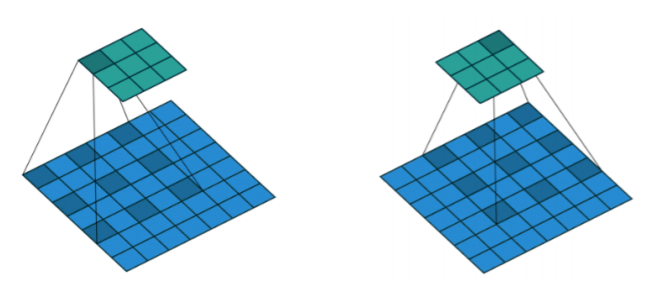
\includegraphics[width=12.0cm]{./8_appendix/img/dilated_conv}
            \caption{Dilated Convolution.}
        \end{center}
    \end{figure}

    \subsubsection{Transposed Convolution}
    Transposed Convolution(転置畳み込み)は,アップサンプリングする際に用いられる手法であり,Deconvolution(逆畳み込み)とも呼ばれる.
    他の畳込み演算と異なり、出力される画像サイズが元の画像よりも大きくなる.
    \begin{figure}[ht]
        \begin{center}
            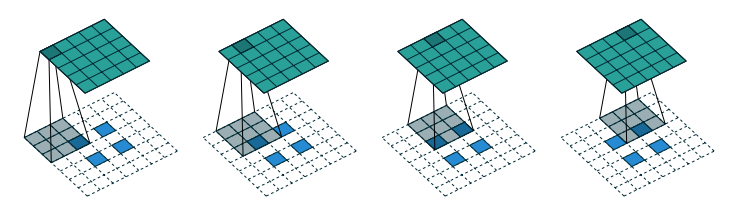
\includegraphics[width=15.0cm]{./8_appendix/img/Deconvolution}
            \caption{Transposed Convolution.}
        \end{center}
    \end{figure}

    \subsubsection{Depthwise Convolution}
    Depthwise ConvolutionはMobileNet\cite{howard2017mobilenets}において採用されている,CNNのパラメータ削減のために導入されている畳み込みの1つである.
    
    通常,畳み込み層では畳込み演算を行った後に各演算結果をチャンネル方向に加算する.
    つまり,入力された全部のチャンネルに対し,単一のフィルタが計算を行っている.
    一方,Depthwise Convolutionでは各チャンネルごとにに対応するフィルタが決まっており,これにより計算量が$1/c_i$となる.
    これはチャンネル間の相関を無視して,単純に空間的な畳込みを実行していることになる.
    
    \subsubsection{Pointwise Convolution}
    Pointwise ConvolutionはDepthwise Convolutionと同様に,MobileNet\cite{howard2017mobilenets}において採用されているCNNのパラメータ削減のために導入されている畳み込みの1つである.
    
    通常の畳み込みではカーネルサイズ$k$を大きくすると,$k$の二乗に比例してパラメータ数が増加する.
    つまり,この$k$を$k=1$と固定することにより,パラメータ数を$1/k^2$とすることができる.
    この畳込みは$k=1$であるため,空間的特徴を捉えずに,チャンネル間の相関構造だけを変化させる特殊な畳み込み演算である.
    また,この畳込みの重要な点として,チャンネル数を変化させることが可能であるため,チャンネル数の辻褄を合わせるような際に良く利用される.
    
    \subsubsection{Depthwise Separable Convolution}
    Depthwise Separable Convolution,MobileNet\cite{howard2017mobilenets}において主に採用されている畳み込み手法である.
    この手法は前述したDepthwise ConvolutionおよびPointwise Convolutionを直列に接続した畳み込みのことを指す.

    Depthwise Convolutionは非常に軽量だが,チャンネル間の構造を捉えることができない上に,出力のチャンネル数が$c_o=c_i$と固定されてしまう.
    そのため,Pointwise Convolutionと縦続接続することでチャンネル側の相関を取り,後に扱いやすいようにチャンネル数の調整を行う.

    パラメータ数はDepthwise ConvolutionおよびPointwise Convolutionの加算となるため,以下のようになる.
    \begin{equation}
        N_p = c_i k^2 + c_i c_o = c_i (k^2 + c_o)
    \end{equation}
    以上により,通常の畳み込みと比べて,Depthwise Separable Convolutionを利用することによるパラメータの削減率は以下の通りである.
    \begin{equation}
        \frac{k^2 + c_o}{k^2 c_o}
    \end{equation}
    これは,ほとんどの層で$c_o>64$かつ$k=3$と設定されていることを踏まえると,全体のパラメータ数がおよそ$1/9$に削減されることを表している.

\subsection{プーリング演算}
    プーリング演算とは,層が深くなるにつれて増大する学習パラメータを削減し,更に畳み込み演算によって得られ特徴量から重要な特徴量を取り出す等の処理を行う演算である.
    この演算を行う層をプーリング層という.
    ここでは,畳み込みニューラルネットワークにおいて最も使われるプーリング演算の例として,マックスプーリング(max pooling)について説明する.
    前述した$4 \times 4$の2階のテンソルに対してマックスプーリング演算を行う.
    このときの演算の概要図を\ref{fig:ex_maxpooling_step_1}-\ref{fig:ex_maxpooling_step_4}に示した.
    \begin{figure}[ht]
      \centering
      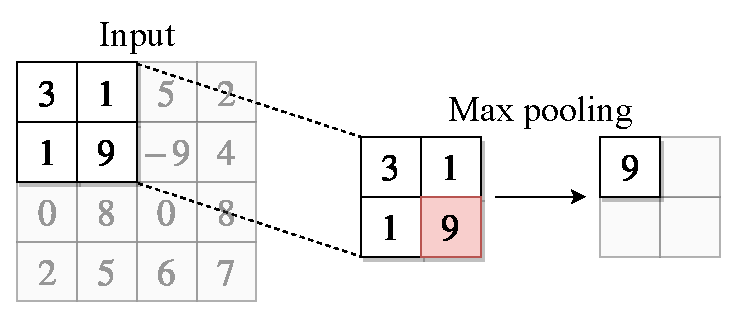
\includegraphics[width=8cm]{8_appendix/img/max_pooling_step1.pdf}
      \caption{Outline of max pooling (Step-1).}
      \label{fig:ex_maxpooling_step_1}
    \end{figure}
    \begin{figure}[ht]
      \centering
      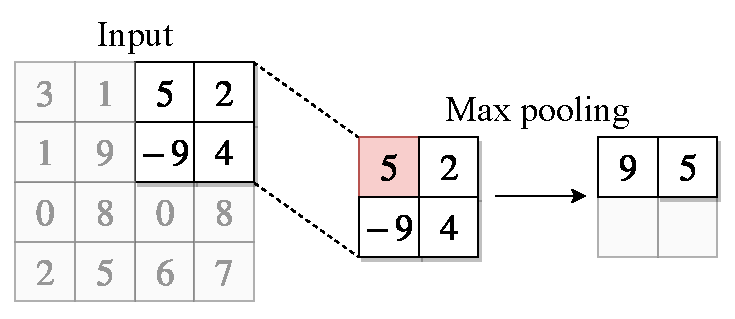
\includegraphics[width=8cm]{8_appendix/img/max_pooling_step2.pdf}
      \caption{Outline of max pooling (Step-2).}
      \label{fig:ex_maxpooling_step_2}
    \end{figure}
    \begin{figure}[ht]
      \centering
      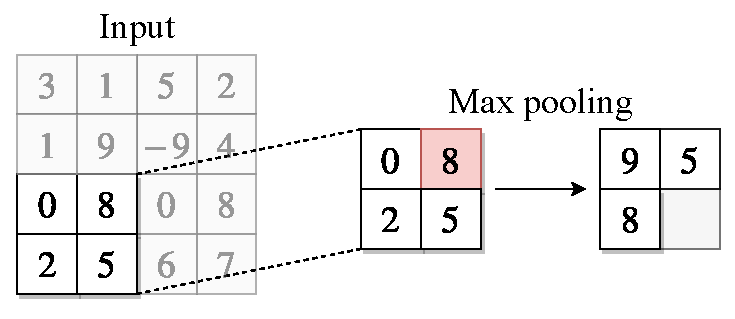
\includegraphics[width=8cm]{8_appendix/img/max_pooling_step3.pdf}
      \caption{Outline of max pooling (Step-3).}
      \label{fig:ex_maxpooling_step_3}
    \end{figure}
    \begin{figure}[ht]
      \centering
      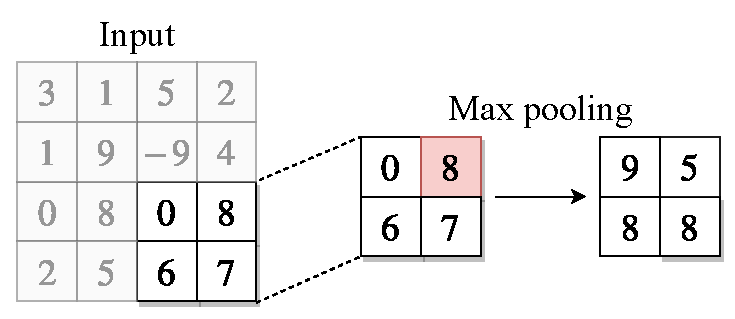
\includegraphics[width=8cm]{8_appendix/img/max_pooling_step4.pdf}
      \caption{Outline of max pooling (Step-4).}
      \label{fig:ex_maxpooling_step_4}
    \end{figure}
    図から明らかなように,入力テンソルから$2 \times 2$の大きさのテンソルを抽出し,その中で最も大きな値を出力する演算である.
    マックスプーリングでの出力は,これを位置をずらしながら繰り返し,その位置ごとにまとめたテンソルとなる.
    また, プーリング層と畳込み層の最も重要な違いは更新されるパラメータを含んでいない点である.
    マックスプーリングはカーネル中の最大値を出力したが,他によく用いられるアベレージプーリングでは,カーネル中の平均値を出力するような設計になっている.

\subsection{様々なプーリング演算}
    前項ではプーリング演算の仕組みについて触れたが,畳み込み層と同じく,近年では様々なプーリング手法が提案されている.
    ここでは,特殊なプーリング演算として,特に本論文で用いる2つのプーリング演算を示す.
    
    \subsubsection{Global Average Pooling}
    Global Average Pooling (GAP)は,入力された特徴マップについて,チャンネルごとに平均を取るプーリング演算である.
    よって,特徴マップは幅および高さを失い,ただのベクトルとして出力される.
    近年は,出力層の手前に配置されるだけではなく,アテンション機構の一部として利用された例などがある\cite{hu2018squeeze}.
    
    \subsubsection{空間ピラミッドプーリング}
    空間ピラミッドプーリング\cite{he2015spatial}(SPP, spatial pyramid pooling)は,入力画像サイズが異なっている場合でも,出力のサイズが同じになるようなプーリング層である.
    このプーリング層では,画像を格子状($1\times1, 2\times2, 4\times4, 16\times16$, ...)に分割し,それぞれでマックスプーリングを行う.
    その後,それぞれの出力値を結合し,結合したベクトルがSPPの出力となる.
    出力サイズはピラミッドのサイズ及びチャンネル数で定義される.
    \begin{figure}[ht]
        \begin{center}
            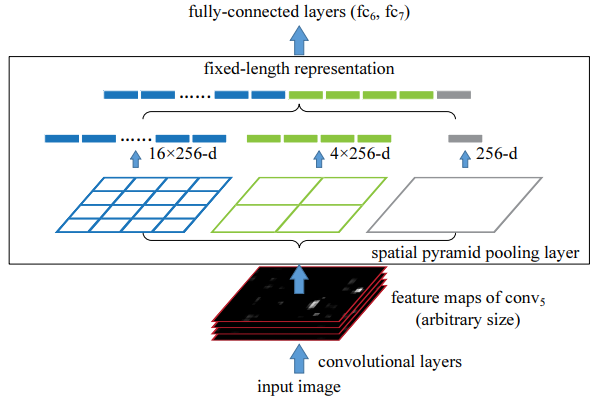
\includegraphics[width=12.0cm]{./8_appendix/img/SPP}
            \caption{spatial pyramid pooling\cite{he2015spatial}.}
        \end{center}
    \end{figure}
    

    

\section{画像認識モデル}
次に,画像認識分野におけるCNNについて説明する.
画像認識分野における課題は,画像中に存在する物体の種類を正確に認識することであり,特に畳み込みニューラルネットワークによる活躍が目覚ましい分野の一つである.
畳み込みニューラルネットワークを用いた手法では,画像を入力とし,多層の畳み込み層を経て特徴量を抽出し,最終的に全結合層を用いて出力を画像に存在する物体の種類(クラス)とするものが多い(\ref{fig:classification}).
\begin{figure}[ht]
  \centering
  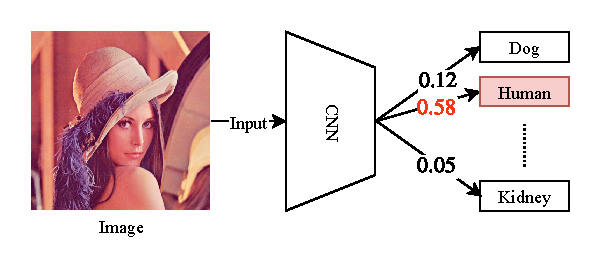
\includegraphics[width=14cm]{8_appendix/img/image_classification.pdf}
  \caption{Classification with CNN.}
  \label{fig:classification}
\end{figure}

本研究において用いるモデルの多くがこれらのモデルに基づいている,
ここでは,その中でも代表的なモデルについて説明する.
\subsubsection{LeNet-5}
    LeNet-5\cite{lecun1998gradient, lecun1999object}は畳み込みニューラルネットワークが注目を集める以前に提案されていた手法であり,6層構造のCNNである.
    LeNetの構造を図\ref{fig:lenet}に示す.
    このモデルは32$\times$32ピクセルのパッチ画像の入力を想定している.
    LeNetで利用されている畳み込み層の基本的な考え方は1989年ごろから提案されていた\cite{lecun1989backpropagation}.
    \begin{figure}[ht]
      \centering
      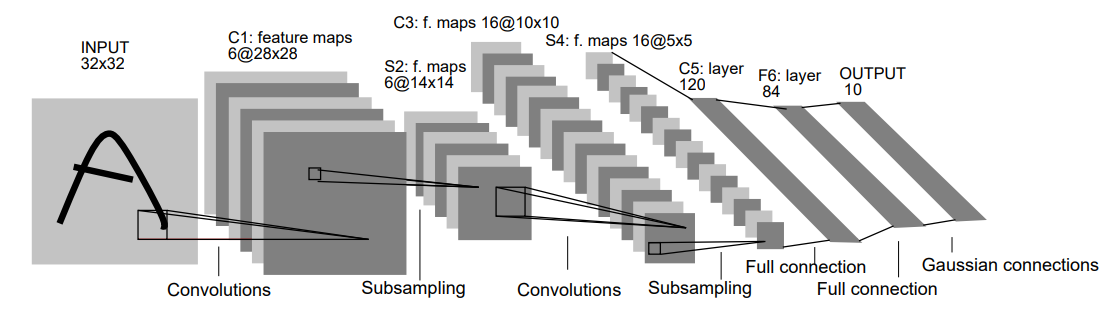
\includegraphics[width=14cm]{8_appendix/img/lenet.png}
      \caption{Architecture of LeNet \cite{lecun1998gradient}.}
      \label{fig:lenet}
    \end{figure}

\subsubsection{AlexNet}
    畳み込みニューラルネットワーク自体は前述のLeNetにて提案されていたが,それが大きく注目されるのは2012年,ImageNet Large Scale Visual Recognition Challenge(ILSVRC)\cite{ILSVRC15}にて,AlexNet\cite{krizhevsky2012imagenet}が画像認識分野において最も優れた成績を示してからである.
    図\ref{fig:alexnet}にネットワーク構造の概要図を示した.
    このモデルは5層の畳み込み層と3層の全結合層で構成され,パラメータ数は約6000万である.
    \begin{figure}[ht]
      \centering
      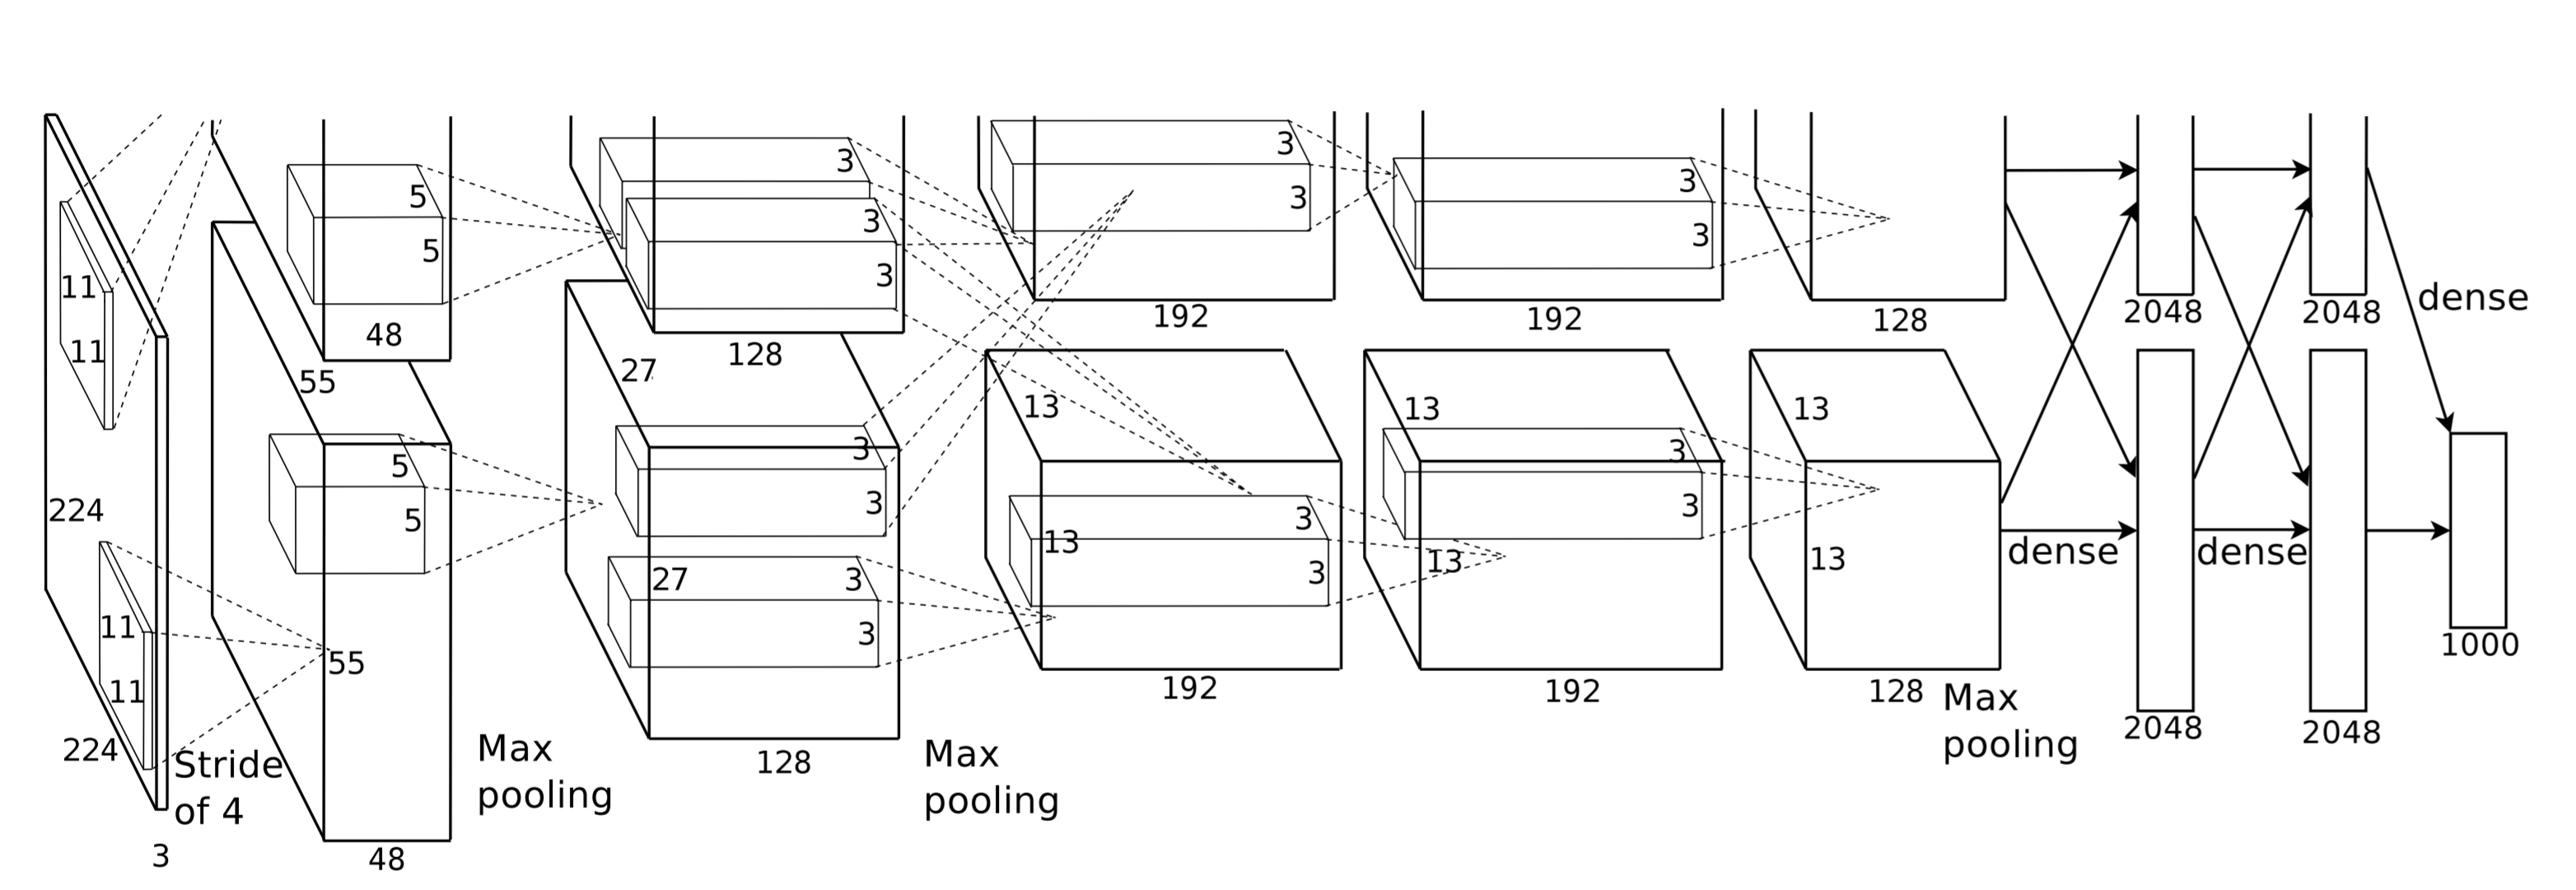
\includegraphics[width=14cm]{8_appendix/img/alexnet.png}
      \caption{Architecture of AlexNet \cite{krizhevsky2012imagenet}.}
      \label{fig:alexnet}
    \end{figure}
    AlexNetはLeNetと異なり,畳み込み層とMax poolingによる畳み込みニューラルネットワークである.
    また活性化関数としてシグモイド関数ではなく,Rectified Linear Unit(ReLU)関数\cite{nair2010rectified}が使われている.
    ReLU関数の導入により,勾配消失問題が改善され,分類精度が向上した.

%\subsubsection{VGG}
%    VGG\cite{simonyan2014very}は2014年にILSVRCで2位になったネットワークであり,AlexNetよりも深いネットワーク構造を持つ.
%    19層のネットワークはVGG-19,16層のネットワークはVGG-16と呼ばれ,パラメータ数は約1億4000万である.

\subsubsection{GoogLeNet}
    GoogLeNet\cite{szegedy2015going}は2014年のILSVRCで1位になったネットワークであり,Inception moduleと呼ばれる複数のフィルタ群により構成されたブロックの組み合わせで構成されている.
    \begin{figure}[ht]
      \centering
      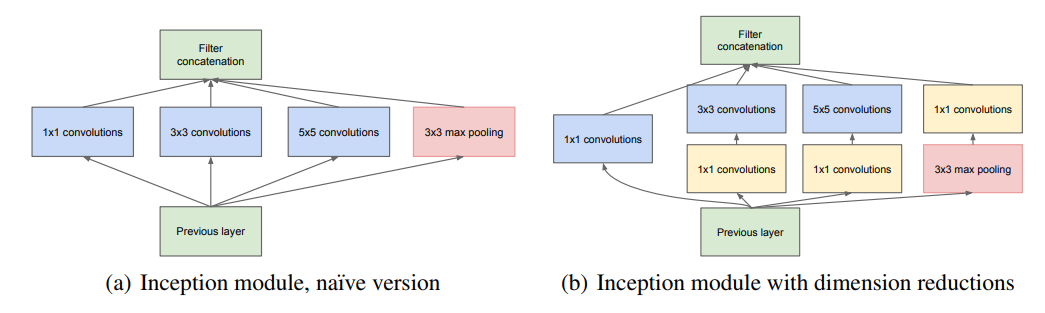
\includegraphics[width=14cm]{8_appendix/img/Inception_module.png}
      \caption{Inception Module \cite{szegedy2015going}.}
    \end{figure}
    Inception moduleは,小さな畳み込みフィルタを並列に並べることで,より少ないパラメータで同等の表現力を実現することが可能である.
    Inception moduleには1*1の畳み込みフィルタが使われているが,このフィルターは次元削減と等価な効果がある.
    \begin{figure}[ht]
      \centering
      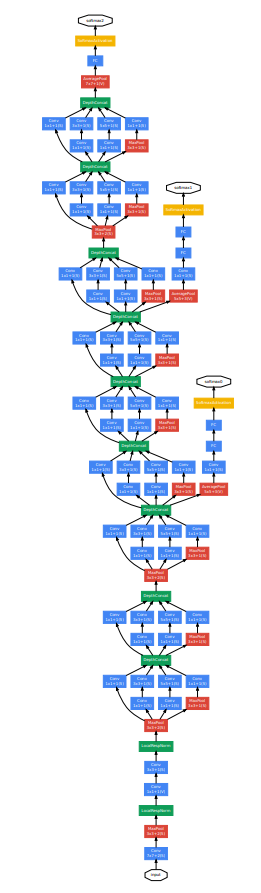
\includegraphics[width=4cm, angle=-90]{8_appendix/img/googlenet.png}
      \caption{Architecture of GoogLeNet \cite{szegedy2015going}.}
    \end{figure}
    
    GoogLeNetのもう一つの特徴として,補助的損失(auxiliary loss)がある.
    GoogLeNetはネットワークの途中から分岐させたサブネットワークにおいてクラス分類を行うような構造を持っており,これによってネットワークの中間層に直接誤差を伝播させ,勾配消失を抑える狙いがある.
    また,複数の損失関数があることにより,アンサンブル学習と同様の効果が得られるため,汎化性能の向上が期待できる.
    ここで,予測時は最終層の出力結果だけを用いることに注意されたい.
    
    このGoogLeNetはその構造の名前を取って一般にinceptionと呼ばれ,構造によってv1からv3まで細かい派生が存在する.
    GoogLeNetはこのv1に該当し,inception v2およびv3はGoogLeNetの畳み込み方法を変更し,モデルを更に多層化したものである.
    前節の畳み込み層の項で述べたが,カーネルサイズ3以上の畳み込みはカーネルサイズ3の畳み込みを複数適用することにより再現できる.
    そこで,v2では図\ref{convFactorization}のようにInception Moduleが改良されている.
    加えて,v2ではバッチ正規化が各層に導入されている.
    \begin{figure}[ht]
      \centering
      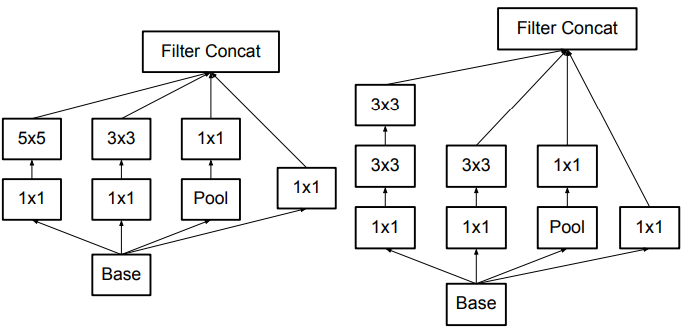
\includegraphics[width=12cm]{8_appendix/img/convFactorization}
      \caption{Factorization of Convolution.The left side is the original Inception Module and the right side is improved for v2 and v3.}
      \label{convFactorization}
    \end{figure}
    
    v3における重要な変更点は,畳み込みの素因数分解である.
    v3では以下の図\ref{improvements_inception}のような$n\times n$畳み込みを$n\times1$畳み込みと$1\times n$畳み込みに分割するモジュールが導入されている.
    これにより,単純な畳込みと比べて計算量が1/3減少する.
    他にも,効率的なグリッドサイズ削減モジュールも導入された.
    これは,従来プーリング層のみで行われていたグリッドサイズ削減を,ストライド2の畳み込みと組み合わせて行うことによって,より安価で効率的なネットワークが実現された.
    \begin{figure}[ht]
      \centering
      \includegraphics[width=12cm]{8_appendix/img/improvements_inception}
      \caption{Various improvements to the Inception Module.}
      \label{improvements_inception}
    \end{figure}

\subsubsection{ResNet}
    GoogLeNetでは補助的損失を用いて勾配消失を防いでいたが,補助的損失は構造が複雑になる上に,モデルのパラメータが増大するなど,様々な課題があった.
    ResNet\cite{he2016deep}ではResidual Block (残差ブロック)を導入することで,100層以上の深い構造であっても学習が可能となった.
    残差ブロックの概要図を図\ref{fig:residual_block}に示した.
    \begin{figure}[ht]
      \centering
      \includegraphics[width=10cm]{8_appendix/img/residual_block.png}
      \caption{Architecture of residual block \cite{he2016deep}.}
      \label{fig:residual_block}
    \end{figure}

    図のように,残差ブロックでは,入力されたデータが二つの経路に分かれる.
    一つが通常の畳み込み演算が行われる経路であり,もう一つが入力データをそのまま出力する経路(ショートカット接続)である.
    このショートカット接続が導入されたモデルの重要な特徴は3つ指摘されている.
    1つは,層をまたがる結合(Identity mapping)によって見かけのネットワークの深さが浅くなり,逆伝播計算時に勾配が減衰していくことを抑える効果をもたらした点である.
    
    そしてもう1つは,ショートカット接続により目的の出力を得るための学習から,残差の学習へと変化させることで,ネットワークが解きやすい問題に帰着させたことである.
    これによって,層が浅い場合でもモデルの高精度化を実現できるようになった.

    たとえば,層の途中で理想の特徴量が得られている場合,畳込みによって,入力と同じ出力を生成する必要があった.
    1つのピクセルに注目すると、各カーネルの各要素との積の総和が入力値と同様になるようなカーネルの重みを学習する必要がある.
    このようなカーネルの重みを学習するのは非常に困難である.
    しかし,残差を学習する場合には,畳込み層は負の値を出力するだけで活性化層で出力は0に是正され,残差ブロックの出力はショートカット接続により加算された入力値となる.
    
    最後は,層を過剰に深くした場合,過学習が発生するようになった点である.
    論文では,過剰に深いモデルを作成し,1202層のモデルでも学習が可能であり,精度が110層のモデル以下となったことを確認している.
    
     現在は,残差ブロックを導入したResNetを元に,様々な改良を施したネットワークの提案がなされている.
     Zagoruykoら\cite{zagoruyko2016wide}は各残差ブロックで増加する畳み込みのフィルタ数を大きくすることで,通常のResNetよりも浅いネットワークで優れた性能を有するを提案した.
     Hanら\cite{han2017deep}は残差ブロック間で急激にフィルタ数を大きくすることで,そのブロックの影響が他と比べて大きくなり,アンサンブル学習としての効果が薄れていると指摘し,各残差ブロックで徐々に畳み込みのフィルタ数を増加するようなネットワークを提案した.

\subsubsection{DenseNet}
    DenseNet\cite{huang2017densely}は,ResNetに似たショートカット結合をもつネットワークであり,その構造をDenseBlockと呼ぶ.
    DenseNetは,ResNet同様にショートカット結合を行っているため,勾配消失が起きにくい.
    ここで,ResNetと同様にショートカット接続を持っているが,足し合わせではなく,特徴量を結合していることの注意されたい.
    また,この構造により層の深さを抑えることができることによりパラメータ数を抑えることに成功している.
    
    \begin{figure}[ht]
      \centering
      \includegraphics[width=10cm]{8_appendix/img/denseblock}
      \caption{Architecture of dense block \cite{huang2017densely}.}
      \label{fig:huang2017densely}
    \end{figure}
    
    チャンネル数kは成長率(Growth rate)と呼ばれ,ハイパーパラメータになる.
    また,図中のBN-ReLU-Convにおいて,異なる色の線はチャンネル方向に結合される.

\subsubsection{MobileNet}
    MobileNet\cite{howard2017mobilenets}はモバイル端末に乗せることのできる軽量かつ高性能なモデルを目標として設計されたCNNである。
    畳み込み層でDepthwise Separable Convolutionを用いることによって通常の畳み込みの1/9ほどに計算量を削減している。
    
    MobileNetは現在に至るまで複数の改良が施されている。
    MobileNet-v2\cite{sandler2018mobilenetv2}ではResNetで使われるResidual Blockを応用したInverted Residualを導入している。
    Residual Blockの計算量の多さを、Depthwise convolutionの前後にPointwise convolutionを挿入する構造を用いて解決している。
    
    MobileNet-v3\cite{howard2019searching}では、Squeeze-and-Exciteモジュールの導入によって、Self-Attentionを行うことによる精度向上を図っている。
    Depthwise convolutionはチャンネルごとに畳み込みを行うため、認識対象に特化した学習が可能になる。

\subsubsection{EfficientNet}
    EfficientNet\cite{tan2019efficientnet}は,モデルの深さ,広さ,解像度(入力画像の大きさ)の3つを調整することによりアーキテクチャにおける最適なモデルスケールアップを実現し,精度向上を達成したモデルである.
    EfficientNetはImageNetを含む5つのデータセットで当時の最高精度を達成した上に,従来のモデルよりもパラメータ数が非常に少ない.
    このモデルは構造が単純であり,転移学習でも効果を発揮する.
    
    EfficientNetはCompound Coefficient(複合係数) 導入し,この比率に従ってモデルの深さ,広さ,解像度の3つを調整されるMBConv\cite{howard2019searching}を多層化することによって構成されている.
    MBConvはMoble Inverted BottleneckにSEモジュールを追加したものであり、MobileNet-v3に採用されている構造である。
    その比率は以下のようになっている.
    \begin{eqnarray}
        \rm{depth:}d &=& \alpha^\phi \\
        \rm{width:}w &=& \beta^\phi \\
        \rm{resolution:}r &=& \gamma^\phi \\
        \rm{s.t.}\ \alpha&\cdot&\beta^{2}\cdot\gamma^{2}\approx2\\
        \alpha &\geq& 1, \beta \geq 1, \gamma \geq 1
    \end{eqnarray}


\section{セマンティックセグメンテーションモデル}
次に,セマンティックセグメンテーション分野におけるCNNについて説明する.
この分野における課題は,画像中に存在する物体を画素毎で精確に分類することである(\ref{fig:semantic_segmentation}).
\begin{figure}[ht]
  \centering
  \includegraphics[width=16cm]{8_appendix/img/semantic_segmentation}
  \caption{Semantic Segmentation with CNN.}
  \label{fig:semantic_segmentation}
\end{figure}
自動運転や医療画像の分野において重要な技術であり、画像分類同様、セマンティックセグメンテーションにおいても CNNは多くの成果を収めている。
ここでは,その中でも代表的なモデルについて説明する.

\subsubsection{Fully Convolutional Networks(FCN)}
    Fully Convolutional Networks(FCN)とは,全ての層が畳み込み層で構成されたニューラルネットワークであり,最終的な出力が,物体の画素ごとのクラス確率となる.
    このネットワークでは,畳み込み層により特徴を抽出した後に,小さくなった画像サイズを出力サイズへ揃えるためのアップサンプリング用の畳み込み層(Deconvolution layer)が導入されている.
    損失には、ピクセル毎のクロスエントロピー誤差の合計を用いている。
    \begin{figure}[ht]
      \centering
      \includegraphics[width=12cm]{8_appendix/img/fcn}
      \caption{FCN architecture \cite{long2015fully}.}
    \end{figure}
    ダウンサンプリングされた特徴マップに対して単純に逆畳み込みを適用するだけでは、出力結果が粗くなってしまう。
    そのため、FCNではスキップ接続を用いて情報ロスが発生する前の情報をアップサンプリング層に入力する。
    \begin{figure}[ht]
      \centering
      \includegraphics[width=12cm]{8_appendix/img/FCNskipconnect}
      \caption{FCN skipconnect architecture \cite{ronneberger2015u}.}
    \end{figure}
    
    このモデルの特徴は全結合層を使わない点であり、全結合層を畳み込み層に置き換えることで、出力を分類クラスではなく二次元マップに変更している。
    FCN以前はネットワーク内に全結合層が存在することにより、固定サイズの画像しか扱うことができなかったが、FCNでは全結合層が存在し
    ないため、あらゆるサイズの画像でセグメンテーションマップが生成できる。

\subsubsection{SegNet}
    SegNet\cite{badrinarayanan2017segnet}はエンコーダ(encoder)部分とデコーダ(decoder)部分で構成されるセマンティックセグメンテーションのためのネットワークである。
    FCNのスキップ接続ではプーリング前の特徴量をアップサンプリング層に入力していた。
    SegNetではエンコーダ部分のマックスプーリング層で採用した値の場所を記録し、デコーダ部分のアップサンプリング時にその位置情報を用いて特徴マップを拡大する。
    これによりデコード時に位置情報が保持され、FCNに比べてメモリ効率が向上した。

\subsubsection{U-Net}
    U-Net\cite{ronneberger2015u}は医療用のセマンティックセグメンテーションで大きな成果を残しているCNNアーキテクチャである.
    U-Netは、様々なスケールの特徴量を出力結果に利用するために,入力に近い層と出力に近い層の間を直接繋げる経路を導入したFCNである.
    \begin{figure}[ht]
      \centering
      \includegraphics[width=12cm]{8_appendix/img/unet.png}
      \caption{U-Net architecture \cite{ronneberger2015u}.}
    \end{figure}

    入力側の特徴量を出力側へ反映する際、FCNやSegNetではチャンネルごとに加算を行っているが、U-Netは特徴量を連結することにより位置情報を保持している。
    これはResNetとDenseNetとの関係と同様である。

\subsubsection{PSPNet}
    PSPNet\cite{zhao2017pyramid}は、Pyramid Pooling Moduleを用いたEncoder–Decoder構造のSemantic Segmentationを行うモデルである。
    Pyramid Pooling Moduleでは、Encoderで抽出された特徴マップに対して、複数の解像度でmax-poolingをかけてそれぞれのスケールで捉えた特徴マップを得る。
    これによって、画像の大域的なコンテキストと小さな部分の情報の両方を拾うことができる。
    
    Pyramid Pooling Moduleの階層数や各階層での特徴マップのサイズは、入力される特徴マップのサイズに合わせて設計する。
    Pyramid Pooling Moduleの階層の数をNとすると、削減後の各特徴マップのチャンネル数は1/Nになる。
    
    論文の例では、階層的に4つの異なるカーネルサイズ(1×1, 2×2, 3×3, 6×6)でmax-poolingを行い、得られた複数スケールの特徴マップを1×1で畳み込んでチャンネル数を削減する。
    \begin{figure}[ht]
      \centering
      \includegraphics[width=15cm]{8_appendix/img/PyramidPoolingModule}
      \caption{Pyramid Pooling Module Architecture\cite{zhao2017pyramid}.}
      \label{fig:unet_architecture}
    \end{figure}
    
    そして、このチャンネル数を削減した特徴マップをバイリニア補間で元の特徴マップと同じサイズにアップサンプリングする。
    アップサンプリングしたこれらの特徴マップを元の特徴マップにチャンネルを追加する形で連結し、大域的なコンテキストと局所的な情報の両方を持った特徴マップとする。
    最終的に、この連結した特徴マップに対して1×1の畳み込みを行ってSemantic Segmentationの結果を得る。

\subsubsection{DeepLab}
    DeepLab\cite{chen2014semantic, chen2017deeplab}は、PSPNetのようにPyramid Pooling Moduleを用いたEncoder–Decoder構造のモデルである。
    DeepLabでは畳み込みにAtrous畳み込み(Dilated Convolution)を利用することで、パラメータの数や計算量を増やすことなく、フィルタの視野を効果的に拡大し、より大きなコンテキストを取り込むことができる。
    DeepLabではこの畳込みをArous spatial pyramid pooling (ASPP)と呼称している。
    他にも、DeepLabでは確率的グラフィカルモデルの手法を組み合わせることで、いくつかのピクセルが孤立して異なるクラスとして予測される問題を解消している。



%TODO?
%\section{敵対的生成モデル}
%\input{./8_appendix/GAN}

%%%%%%%%%%%%%%%%%%%%%%%%%%%%%%%%%
\chapter{画像レジストレーションの基礎}

\section{画像の変形手法}
\label{appendix_transformation}
% TODO
% TPS変換
% DVF
% 相互相関
画像のレジストレーションの方法に関わらず、画像の変形は画像レジストレーションに必要な要素である。

%画像の変形技術は大別して線形変形および非線形変形の2種類がある。
%本節では画像変形手法について上記の二つの方法を述べる。

\subsection{アフィン変換}
    アフィン変換は幾何平面上で定義される画像に対する最も基本的な変形方法である。
    この変換は、平行移動、拡大縮小、回転、せん断変形を$3\times 3$行列を用いて行われる。
    変換前の座標を$(x,y)$、変形後の座標を$(x^{\prime},y^{\prime})$とすると、アフィン変換は次式で表すことができる。
    \begin{equation}
        \left(\begin{array}{l}
        x^{\prime} \\
        y^{\prime} \\
        1
        \end{array}\right)
        =
        \left(\begin{array}{lll}
        a & b & c\\
        d & e & f\\
        0 & 0 & 1
        \end{array}\right)
        \left(\begin{array}{l}
        x \\
        y \\
        1
        \end{array}\right)
    \end{equation}
    このアフィン変換は、変形によって図形の面積が不変であり、任意のピクセル同士の順序や相対距離が不変である。

    \subsubsection{平行移動}
        アフィン変換において最も基本的な変換は平行移動である。

        \begin{figure}[htbp]
            \begin{minipage}{0.5\hsize}
                \begin{center}
                    \includegraphics[width=50mm]{./8_appendix/img/imori.jpg}
                \end{center}
                \caption{元画像}
            \end{minipage}
            \begin{minipage}{0.5\hsize}
                \begin{center}
                    \includegraphics[width=50mm]{./8_appendix/img/imori_Translation.jpg}
                \end{center}
                \caption{x方向に+30、y方向に-30平行移動した後の画像}
            \end{minipage}
        \end{figure}

        平行移動は、x,yそれぞれの移動量を$(d_x, d_y)$とすると、以下の式で定義できる。
        \begin{equation}
            \left(\begin{array}{l}
            x^{\prime} \\
            y^{\prime} \\
            1
            \end{array}\right)
            =
            \left(\begin{array}{lll}
            1 & 0 & d_x\\
            0 & 1 & d_y\\
            0 & 0 & 1
            \end{array}\right)
            \left(\begin{array}{l}
            x \\
            y \\
            1
            \end{array}\right)
        \end{equation}

    \subsubsection{拡大・縮小}
        拡大縮小は、x,yそれぞれの倍率を$S_x, S_y$とすると、以下の式で定義できる。
        \begin{equation}
            \left(\begin{array}{l}
            x^{\prime} \\
            y^{\prime} \\
            1
            \end{array}\right)
            =
            \left(\begin{array}{lll}
            S_x & 0 & 0\\
            0 & S_y & 0\\
            0 & 0 & 1
            \end{array}\right)
            \left(\begin{array}{l}
            x \\
            y \\
            1
            \end{array}\right)
        \end{equation}
        \begin{figure}[htbp]
            \begin{minipage}{0.5\hsize}
                \begin{center}
                    \includegraphics[width=50mm]{./8_appendix/img/imori.jpg}
                \end{center}
                \caption{元画像}
            \end{minipage}
            \begin{minipage}{0.5\hsize}
                \begin{center}
                    \includegraphics[width=65mm]{./8_appendix/img/imori_Scale.jpg}
                \end{center}
                \caption{x方向に1.3倍、y方向に0.8倍にリサイズした後の画像}
            \end{minipage}
        \end{figure}

        また、このとき$S_x, S_y$を負の値にすることによって、反転処理を実現することができる。
        このような処理を鏡映と呼び、x軸に対して対称の画像を作成する場合には$S_y$を負の値に、y軸に対して対称の画像を作成する場合には$S_x$を負の値にする必要がある。
        このとき、単純に反転を行った場合には画素は画像の範囲から逸脱することに注意する必要がある。
        そのため、計算機上で反転を行う場合には、単純に格納される配列を逆順にする操作を行う場合が多い。

    \subsubsection{回転}
        回転は、角度$\theta$を用いて以下の式で定義できる。
        \begin{equation}
            \left(\begin{array}{l}
            x^{\prime} \\
            y^{\prime} \\
            1
            \end{array}\right)
            =
            \left(\begin{array}{lll}
            \cos{\theta} & -\sin{\theta} & 0\\
            \sin{\theta} & \cos{\theta} & 0\\
            0 & 0 & 1
            \end{array}\right)
            \left(\begin{array}{l}
            x \\
            y \\
            1
            \end{array}\right)
        \end{equation}
        \begin{figure}[htbp]
            \begin{minipage}{0.5\hsize}
                \begin{center}
                    \includegraphics[width=50mm]{./8_appendix/img/imori.jpg}
                \end{center}
                \caption{元画像}
            \end{minipage}
            \begin{minipage}{0.5\hsize}
                \begin{center}
                    \includegraphics[width=50mm]{./8_appendix/img/imori_Rotate.jpg}
                \end{center}
                \caption{原点を中心として30度回転させた画像}
            \end{minipage}
            \begin{minipage}{0.5\hsize}
                \begin{center}
                    \includegraphics[width=50mm]{./8_appendix/img/imori_Rotate_center.jpg}
                \end{center}
                \caption{画像中心を原点として30度回転させた画像}
            \end{minipage}
        \end{figure}
        また、この場合回転中心は原点、つまり画像の左上になってしまうため、画像中心を原点として回転させる場合には平行移動と上手く組み合わせて利用する必要がある。
    
    \subsubsection{せん断}
        画像を斜め方向に伸ばすような変形をせん断変形と呼ぶ。
        せん断変形は、移動量$(d_x, d_y)$を用いて以下の式で定義できる。
        \begin{equation}
            \left(\begin{array}{l}
            x^{\prime} \\
            y^{\prime} \\
            1
            \end{array}\right)
            =
            \left(\begin{array}{lll}
            1 & \frac{d_x}{h} & 0\\
            0 & 1 & 0\\
            0 & 0 & 1
            \end{array}\right)
            \left(\begin{array}{l}
            x \\
            y \\
            1
            \end{array}\right)
            \label{Xsharing}
        \end{equation}

        \begin{equation}
            \left(\begin{array}{l}
            x^{\prime} \\
            y^{\prime} \\
            1
            \end{array}\right)
            =
            \left(\begin{array}{lll}
            1 & 0 & 0\\
            \frac{d_y}{h} & 1 & 0\\
            0 & 0 & 1
            \end{array}\right)
            \left(\begin{array}{l}
            x \\
            y \\
            1
            \end{array}\right)
            \label{Ysharing}
        \end{equation}
        ここで$h$および$w$は画像の高さおよび幅を表す。

        このとき、式(\ref{Xsharing})のような$x$方向に$d_x$だけ引き伸ばしたような画像はX-sharingと呼ばれ、式(\ref{Ysharing})のような$y$方向に$d_y$だけ引き伸ばしたような画像はY-sharingと呼ばれる。
        \begin{figure}[htbp]
            \begin{minipage}{0.5\hsize}
                \begin{center}
                    \includegraphics[width=50mm]{./8_appendix/img/imori.jpg}
                \end{center}
                \caption{元画像}
            \end{minipage}
            \begin{minipage}{0.5\hsize}
                \begin{center}
                    \includegraphics[width=50mm]{./8_appendix/img/imori_xshar.jpg}
                \end{center}
                \caption{x方向に30ピクセルだけ引き伸ばした画像}
            \end{minipage}
            \begin{minipage}{0.5\hsize}
                \begin{center}
                    \includegraphics[width=50mm]{./8_appendix/img/imori_yshar.jpg}
                \end{center}
                \caption{y方向に30ピクセルだけ引き伸ばした画像}
            \end{minipage}
        \end{figure}

    \subsubsection{アフィン変換行列の逆行列}
        アフィン変換によって変形した画像を元の画像に戻す際には、アフィン変換行列の逆行列を求める必要がある。
        通常の3次正方元行列と異なり、アフィン変換行列の逆行列は以下のように比較的簡単に求めることができる。
        \begin{align}
            \left(
            \begin{array}{ccc}
                a&b&t_x\\ c&d&t_y\\ 0&0&1 
            \end{array}
            \right)^{-1} 
        &=  \left( 
                \left(
                \begin{array}{ccc}
                    1&0&t_x\\ 0&1&t_y\\ 0&0&1 
                \end{array}
                \right)
                \left(
                \begin{array}{ccc}
                    a&b&0\\ c&d&0\\ 0&0&1
                \end{array}
                \right)
            \right) ^ {-1} \\ 
        &=  \left(
            \begin{array}{ccc}
                a&b&0\\ c&d&0\\ 0&0&1
            \end{array}\right)^{-1}
            \left(
            \begin{array}{ccc}
                1&0&t_x\\ 0&1&t_y\\ 0&0&1
            \end{array}\right)^{-1} \\
        &= \left(
            \begin{array}{ccc}
                d/\Delta{}&-b/\Delta{}&0\\ -c/\Delta{}&a/\Delta{}&0\\ 0&0&1 
            \end{array}
            \right)
            \left(
            \begin{array}{ccc}
                1&0&-t_x\\ 0&1&-t_y\\ 0&0&1
            \end{array}\right)\\
        &= \left(
            \begin{array}{ccc}
            d/\Delta{}&-b/\Delta{}&(-dt_x+bt_y)/\Delta{}\\ -c/\Delta{}&a/\Delta{}&(ct_x-at_y)/\Delta{}\\ 0&0&1
            \end{array}
            \right)
        \end{align}
        

\subsection{射影変換}

\subsection{非線形変形}
    以上のような線形変換では実現できないような複雑な位置合わせを行う場合は非線形変換を行う必要がある.
    \subsubsection{B-spline法}
        非線形位置合わせではB-spline法がよく用いられる.
        ある画素に注目した際に, 近傍4つの制御点から成る変位場とB-spline関数の掛け合わせによって変形が行われる.
        制御点を等間隔$\delta$に設定し, 変位場を$\phi\left(i+m, j+n\right)$とすると, B-spline曲線を用いた非線形変換は以下のように定義される.
        \begin{eqnarray} 
        \mu(x, y)&=&\sum_{m=0}^{3} \sum_{n=0}^{3} B_{m}(u(x)) B_{n}(v(y)) \phi\left(i+m, j+n\right)\\
        i&=&\left|\frac{x}{\delta}\right|-1, j=\left|\frac{y}{\delta}\right|-1\\
        u(x)&=&\frac{x}{\delta}-\left|\frac{x}{\delta}\right|, v(y)=\frac{y}{\delta}-\left|\frac{y}{\delta}\right|\\
        B_{0}(s)=\frac{(1-s)^{3}}{6}, B_{1}(s)&=&\frac{3 S^{3}-6 S^{2}+4}{6}, B_{2}(s)=\frac{-3 S^{3}+3 S^{2}+3 s+1}{6}, B_{3}(s)=\frac{S^{3}}{6}
        \end{eqnarray}
            \begin{figure}[ht]
            \begin{center}
              \includegraphics[width=10.0cm]{./8_appendix/img/spline}
            \caption{スプライン曲線を用いた画像変形の例\ (a)元画像\ (b)(c)変形操作\ (d)変形後の画像}
            \label{}
            \end{center}
        \end{figure}

    \subsubsection{Thin-Plate-spline法}

\subsection{Displacement Vector Field}

% 引用
\bibliography{ref}

\end{document}